% Options for packages loaded elsewhere
\PassOptionsToPackage{unicode}{hyperref}
\PassOptionsToPackage{hyphens}{url}
\PassOptionsToPackage{dvipsnames,svgnames,x11names}{xcolor}
%
\documentclass[
  11pt,
]{book}
\usepackage{amsmath,amssymb}
\usepackage{lmodern}
\usepackage{iftex}
\ifPDFTeX
  \usepackage[T1]{fontenc}
  \usepackage[utf8]{inputenc}
  \usepackage{textcomp} % provide euro and other symbols
\else % if luatex or xetex
  \usepackage{unicode-math}
  \defaultfontfeatures{Scale=MatchLowercase}
  \defaultfontfeatures[\rmfamily]{Ligatures=TeX,Scale=1}
\fi
% Use upquote if available, for straight quotes in verbatim environments
\IfFileExists{upquote.sty}{\usepackage{upquote}}{}
\IfFileExists{microtype.sty}{% use microtype if available
  \usepackage[]{microtype}
  \UseMicrotypeSet[protrusion]{basicmath} % disable protrusion for tt fonts
}{}
\makeatletter
\@ifundefined{KOMAClassName}{% if non-KOMA class
  \IfFileExists{parskip.sty}{%
    \usepackage{parskip}
  }{% else
    \setlength{\parindent}{0pt}
    \setlength{\parskip}{6pt plus 2pt minus 1pt}}
}{% if KOMA class
  \KOMAoptions{parskip=half}}
\makeatother
\usepackage{xcolor}
\usepackage{longtable,booktabs,array}
\usepackage{calc} % for calculating minipage widths
% Correct order of tables after \paragraph or \subparagraph
\usepackage{etoolbox}
\makeatletter
\patchcmd\longtable{\par}{\if@noskipsec\mbox{}\fi\par}{}{}
\makeatother
% Allow footnotes in longtable head/foot
\IfFileExists{footnotehyper.sty}{\usepackage{footnotehyper}}{\usepackage{footnote}}
\makesavenoteenv{longtable}
\usepackage{graphicx}
\makeatletter
\def\maxwidth{\ifdim\Gin@nat@width>\linewidth\linewidth\else\Gin@nat@width\fi}
\def\maxheight{\ifdim\Gin@nat@height>\textheight\textheight\else\Gin@nat@height\fi}
\makeatother
% Scale images if necessary, so that they will not overflow the page
% margins by default, and it is still possible to overwrite the defaults
% using explicit options in \includegraphics[width, height, ...]{}
\setkeys{Gin}{width=\maxwidth,height=\maxheight,keepaspectratio}
% Set default figure placement to htbp
\makeatletter
\def\fps@figure{htbp}
\makeatother
\setlength{\emergencystretch}{3em} % prevent overfull lines
\providecommand{\tightlist}{%
  \setlength{\itemsep}{0pt}\setlength{\parskip}{0pt}}
\setcounter{secnumdepth}{5}
\usepackage{booktabs}
\usepackage{amsthm}
\usepackage{float}
\usepackage{fontspec}

%\setmainfont{cmunrm.otf}

\makeatletter
\def\thm@space@setup{%
  \thm@preskip=8pt plus 2pt minus 4pt
  \thm@postskip=\thm@preskip
}
\makeatother

\usepackage{a4wide}
\setlength{\parindent}{0in}
\setlength{\parskip}{1ex}
% grootte van de pagina


\setlength{\topmargin}{-0.25in}
\setlength{\oddsidemargin}{0.25in}
\setlength{\evensidemargin}{0.25in}
\setlength{\textwidth}{6.0in}
\setlength{\textheight}{9.0in}
\ifLuaTeX
  \usepackage{selnolig}  % disable illegal ligatures
\fi
\usepackage[]{natbib}
\bibliographystyle{apalike}
\IfFileExists{bookmark.sty}{\usepackage{bookmark}}{\usepackage{hyperref}}
\IfFileExists{xurl.sty}{\usepackage{xurl}}{} % add URL line breaks if available
\urlstyle{same} % disable monospaced font for URLs
\hypersetup{
  pdftitle={Biological Aspects of Biodanza},
  pdfauthor={Lieven Clement},
  colorlinks=true,
  linkcolor={blue},
  filecolor={Maroon},
  citecolor={blue},
  urlcolor={blue},
  pdfcreator={LaTeX via pandoc}}

\title{Biological Aspects of Biodanza}
\author{Lieven Clement}
\date{2022-10-13}

\begin{document}
\maketitle

{
\hypersetup{linkcolor=}
\setcounter{tocdepth}{2}
\tableofcontents
}
\hypertarget{licence-and-links}{%
\chapter*{Licence and links}\label{licence-and-links}}
\addcontentsline{toc}{chapter}{Licence and links}

This work is shared under the
CC BY-NC-SA 4.0 licence.

You may use the material for non-commercial purposes.

You are allowed to copy and redistribute the material in any medium or format and remix, transform, and build upon the material provided that you give proper credit to the author.

If you remix, transform, or build upon the material, you must distribute your contributions under the same license as the original.

A pdf version of this ebook can be found here: \href{https://biodanzabrugge.be/biologicalAspectsBiodanza/Biological-Aspects-of-Biodanza.pdf}{Biological-Aspects-of-Biodanza.pdf}

\hypertarget{intro}{%
\chapter{Introduction}\label{intro}}

Biodanza uses the power of music and movement in an affective group to evoke vivencia, a deep experience with a strong bodily component. This triggers positive processes of change that continue well beyond the Biodanza sessions and work through in our daily life.

\begin{figure}

{\centering 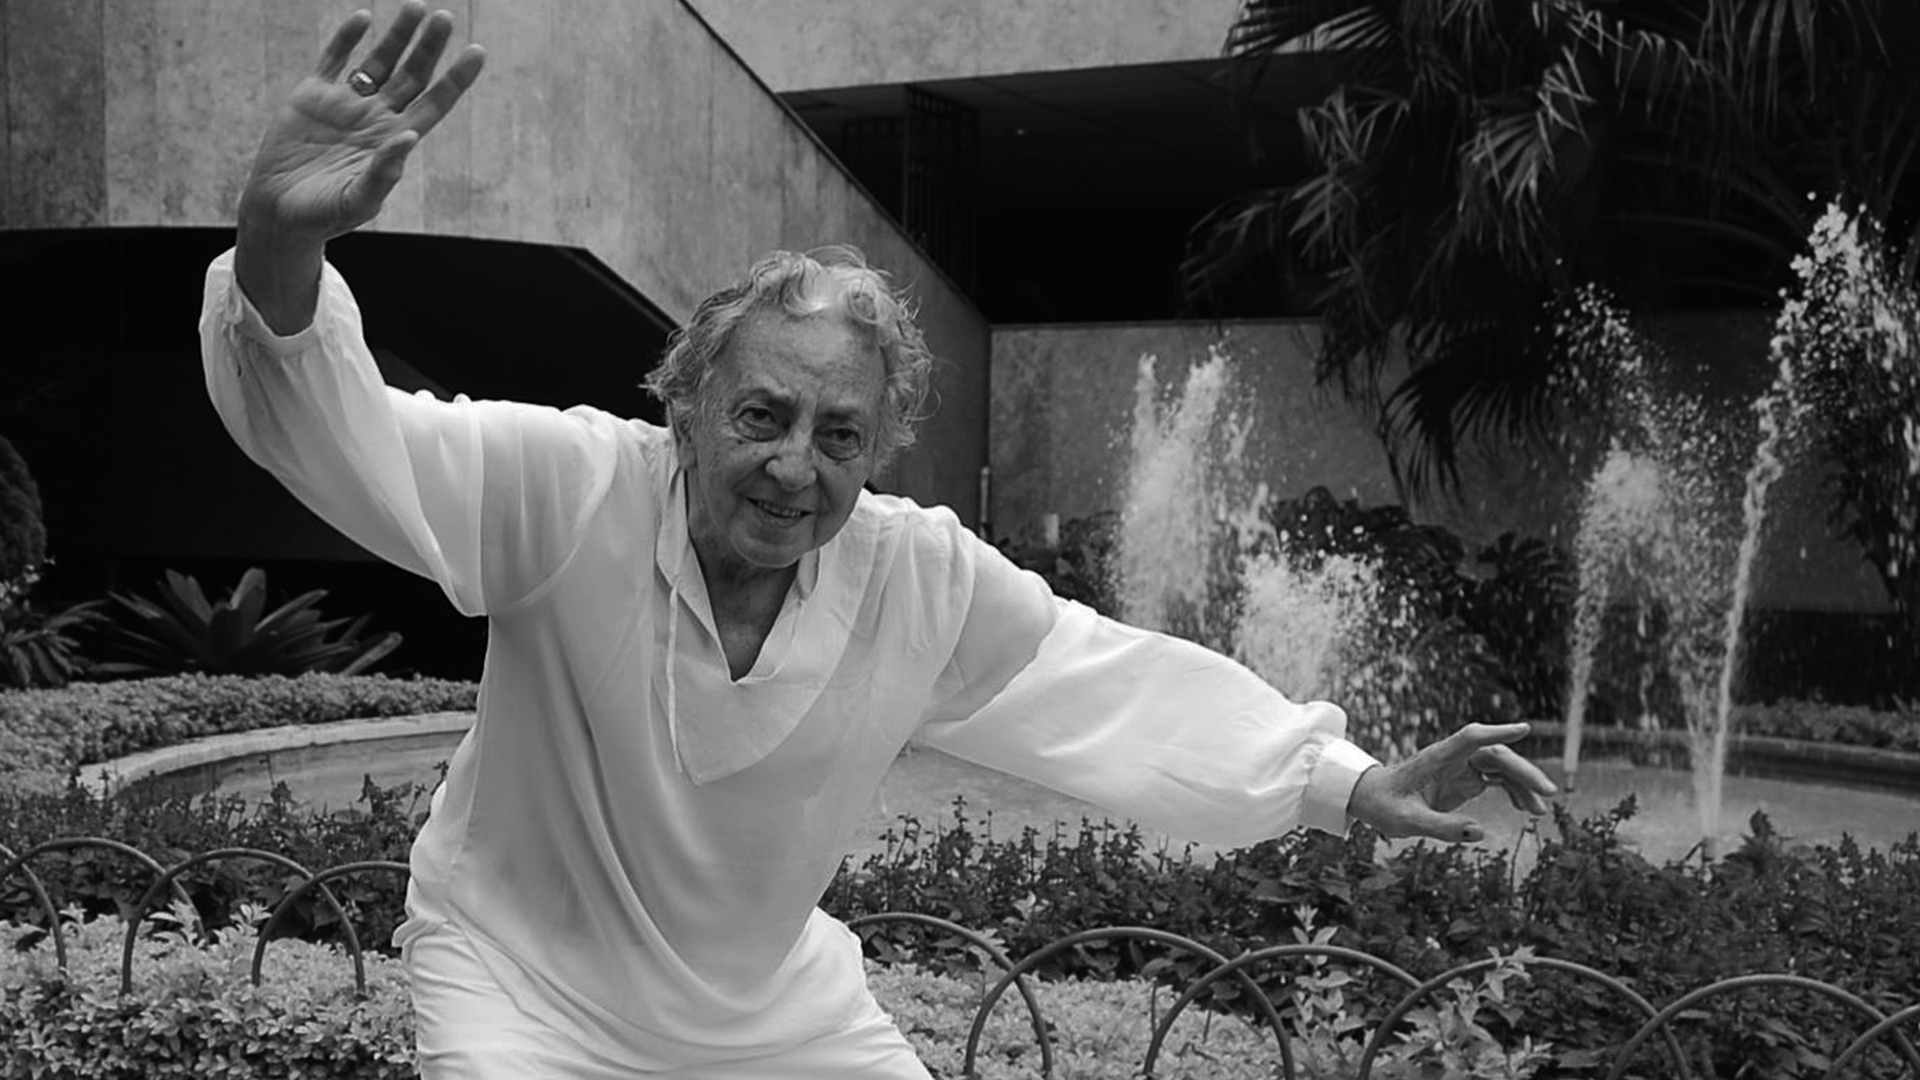
\includegraphics[width=0.45\linewidth]{./figs/rolando} 

}

\caption{Rolando Toro, the developer of Biodanza}\label{fig:rolandoToro}
\end{figure}

For Rolando Toro, the inventor and developer of Biodanza, the most important thing was: ``Vivencia, Vivencia, Vivencia''. Indeed, experiencing life through dance, music and movement enables us to deeply connect with your inner self, each other and the whole. Biodanza lets us feel that life is one and this through a deep and intense bodily experience that is bypassing our cognitive mind.

With his system of Biodanza Rolando anticipated against the degeneration of humanity and the human society he observed during the second world war. For Rolando it was clear that modern women and men suffer from a disease he called ``society''. Our current society brings us far from our natural state of being, feeling, affection and sympathy, which can trigger anyone to extreme acts of violence and cruelty.

Therefore, he has developed his system of Biodanza from a nostalgia to love. A system that disseminates love and hope. A system that enables an affective re-education and that invites us to take part in a new way of live nourished by intense experiences.

Rolando was a passionate scientist and professor in psychology. He developed Biodanza from his own experiences and realized early on that his system has a strong foundation in the life sciences. During his development, he has also been inspired by the founders of modern dance and by primal people who still lay a deep meaning in each movement.

By learning again how to add meaning to each of our movements, we ``re-humanize'' and can find how to truly live life deeply connected with the beauty of nature surrounding us.

\begin{figure}

{\centering 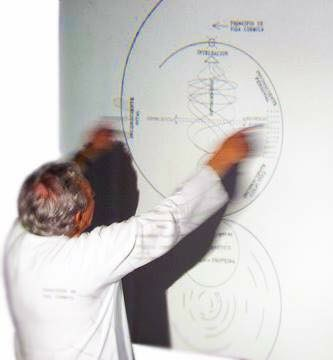
\includegraphics[width=0.45\linewidth]{./figs/rolandoAndModel} 

}

\caption{Rolando Toro explaining his Model of Biodanza}\label{fig:rolandoModel}
\end{figure}

Rolando has laid the foundation of his system during his career as a psychologist/researcher where he discovered the true impact of exercises that stimulate regression and identity, the first axis in his system. As opposed to the conventional mode of action in psychiatry, which has a starting point that is in essence symptomatic, for instance by dosing hormones or neurotransmitters that a patient is lacking, Rolando developed the vision that we could use external stimuli (ecofactors) such as music, movement, touch, caressing, encounters and dance to stimulate our body to produce these substances internally. And this, by stimulating our body to tap into its genetic potential, which can promote immense growth.

Growth and learning in Biodanza happens as how children learn: by seeing, imitating, experiencing and repetition, and, this deeply embedded in a stimulating environment with positive reinforcement.

\hypertarget{definition-of-biodanza}{%
\section{Definition of Biodanza}\label{definition-of-biodanza}}

Rolando coined the term ``Biodanza'', which is a contraction of ``bios'', the Greek word for ``life'', and, ``danza'' the Italian word for dance. Here, the word ``danza'' is used in its original sense of ``natural movement'' that is full of meaning and well-connected with our emotions.

Marcelo Mur defines Biodanza in its most simple form as a system of moderate movement and stimulation of sociability.
Rolando Toro as a poetry of encounter. Indeed, all exercises can be seen as a preparation on the encounter with oneself, each other and the whole.

In Rolando's more academic definition Biodanza is a system of human integration, of organic renewal, of affective re-education and of re-learning the original functions of life.

The methodology of Biodanza consists of inducing integrating vivencia through music, singing, movement and encounters in an affective group.

\hypertarget{vivencia}{%
\subsection{Vivencia}\label{vivencia}}

The concept of vivencia is key to understand the method of Biodanza.

Vivencia is an intense sensation of living, here and now, with a strong component of total organic sensation that elicits a strong awareness of our bodily existence. It is a manifestation of being that precedes consciousness.
Vivencia are passing experiences, e.g.~vivencia of fullness, of safety, of delight.
The awareness of experiencing vivencia can come instantly or at a later moment and often gives rise to deep emotions.

We do not have to try to rationalize our vivencia.
They can be seen as manifestations of our bodily wisdom and spontaneously initiate integration and learning by experience.
They are transformative experiences and are the most important instrument of the method of Biodanza.

\hypertarget{human-integration}{%
\subsection{Human Integration}\label{human-integration}}

Through vivencia a strong connection with life is established, which induces the integration with oneself, the human species and the universe.

The integration with oneself restores our psycho-physical unity, i.e.~the unity of the internal/psychic and external/physical world.

Integration with our fellow humans restores the connection within our species as a biological unity.

Integration with the universe re-unites us with nature and restores our intimate relation with the entire biosphere.
It lets us re-experience the deep connection of ourselves as part of the cosmos.

By restoring this connection to life, we can re-experience life to its very existence, here and now, which promotes a deep conscious awakening.

\hypertarget{organic-renewal}{%
\subsection{Organic Renewal}\label{organic-renewal}}

Biological systems possess the unique capacity of self-replication and self-organisation. However, stress has a profound impact on cell and tissue maintenance and regeneration.

With Biodanza exercises that aim for regression and transcendence, we slow down our movements, lower our state of control and evoke a deep state of rest. This state is essential to switch on restoration and regeneration, and, reinforces homeostasis, i.e.~our bodies mechanism to maintain its equilibrium despite the oscillations in our environment.

\hypertarget{affective-re-education}{%
\subsection{Affective Re-education}\label{affective-re-education}}

In Biodanza many exercises stimulate and elicit affection and harmony, which can work through in our daily life by bringing harmony in our relation with ourselves, among each-other and with our environment.

\hypertarget{re-learning-of-the-original-functions-of-life}{%
\subsection{Re-learning of the Original Functions of Life}\label{re-learning-of-the-original-functions-of-life}}

Biodanza practice also reconnects us with our primal instincts, which are suppressed in our modern society and are often viewed as irrational behavior.
However, our instincts can be viewed as the biological wisdom of our species, which evolved for survival and maintenance of our species. By reconnecting ourselves with our innate impulses, we also restores harmony from within.

\hypertarget{sectionBiocentricPrinciple}{%
\section{Biocentric Principle}\label{sectionBiocentricPrinciple}}

The biocentric principle is at the heart of Rolando Torro's system of Biodanza. The biocentric principle considers the universe as the matrix of life, i.e.~a self-organizing structure that is building life. So not only living organisms, but, rather the entire cosmos is viewed as a massive living hologram.

This view invites people to radically rethink their relationship as a human being with the entire biosphere. Indeed, life itself becomes intrinsically sacred, which probes us to put all of life, and thus the entire universe, at the heart of our weltanschauung.

To me, it seems an invitation to gravitate from humanism, with human beings at its center, back to the view of primal cultures where the environment we are living in is not seen as the stage upon which we tread, but as an entity with whom we can communicate and build a deep intimate relationship.

Vivencia is the unique path to experience the Biocentric Principle and to genuinely become aware of it. This not through our mind, but, through that deeper knowledge that lies hidden in our inner self, ready to be touched by the intimate vivencial experience.

\hypertarget{sectionModelOfBiodanza}{%
\section{Model of Biodanza}\label{sectionModelOfBiodanza}}

Rolando Toro developed a scheme of his model of Biodanza that summarizes its foundation in the life sciences and its methodology, which is displayed in Figure \ref{fig:model}.

\begin{figure}

{\centering 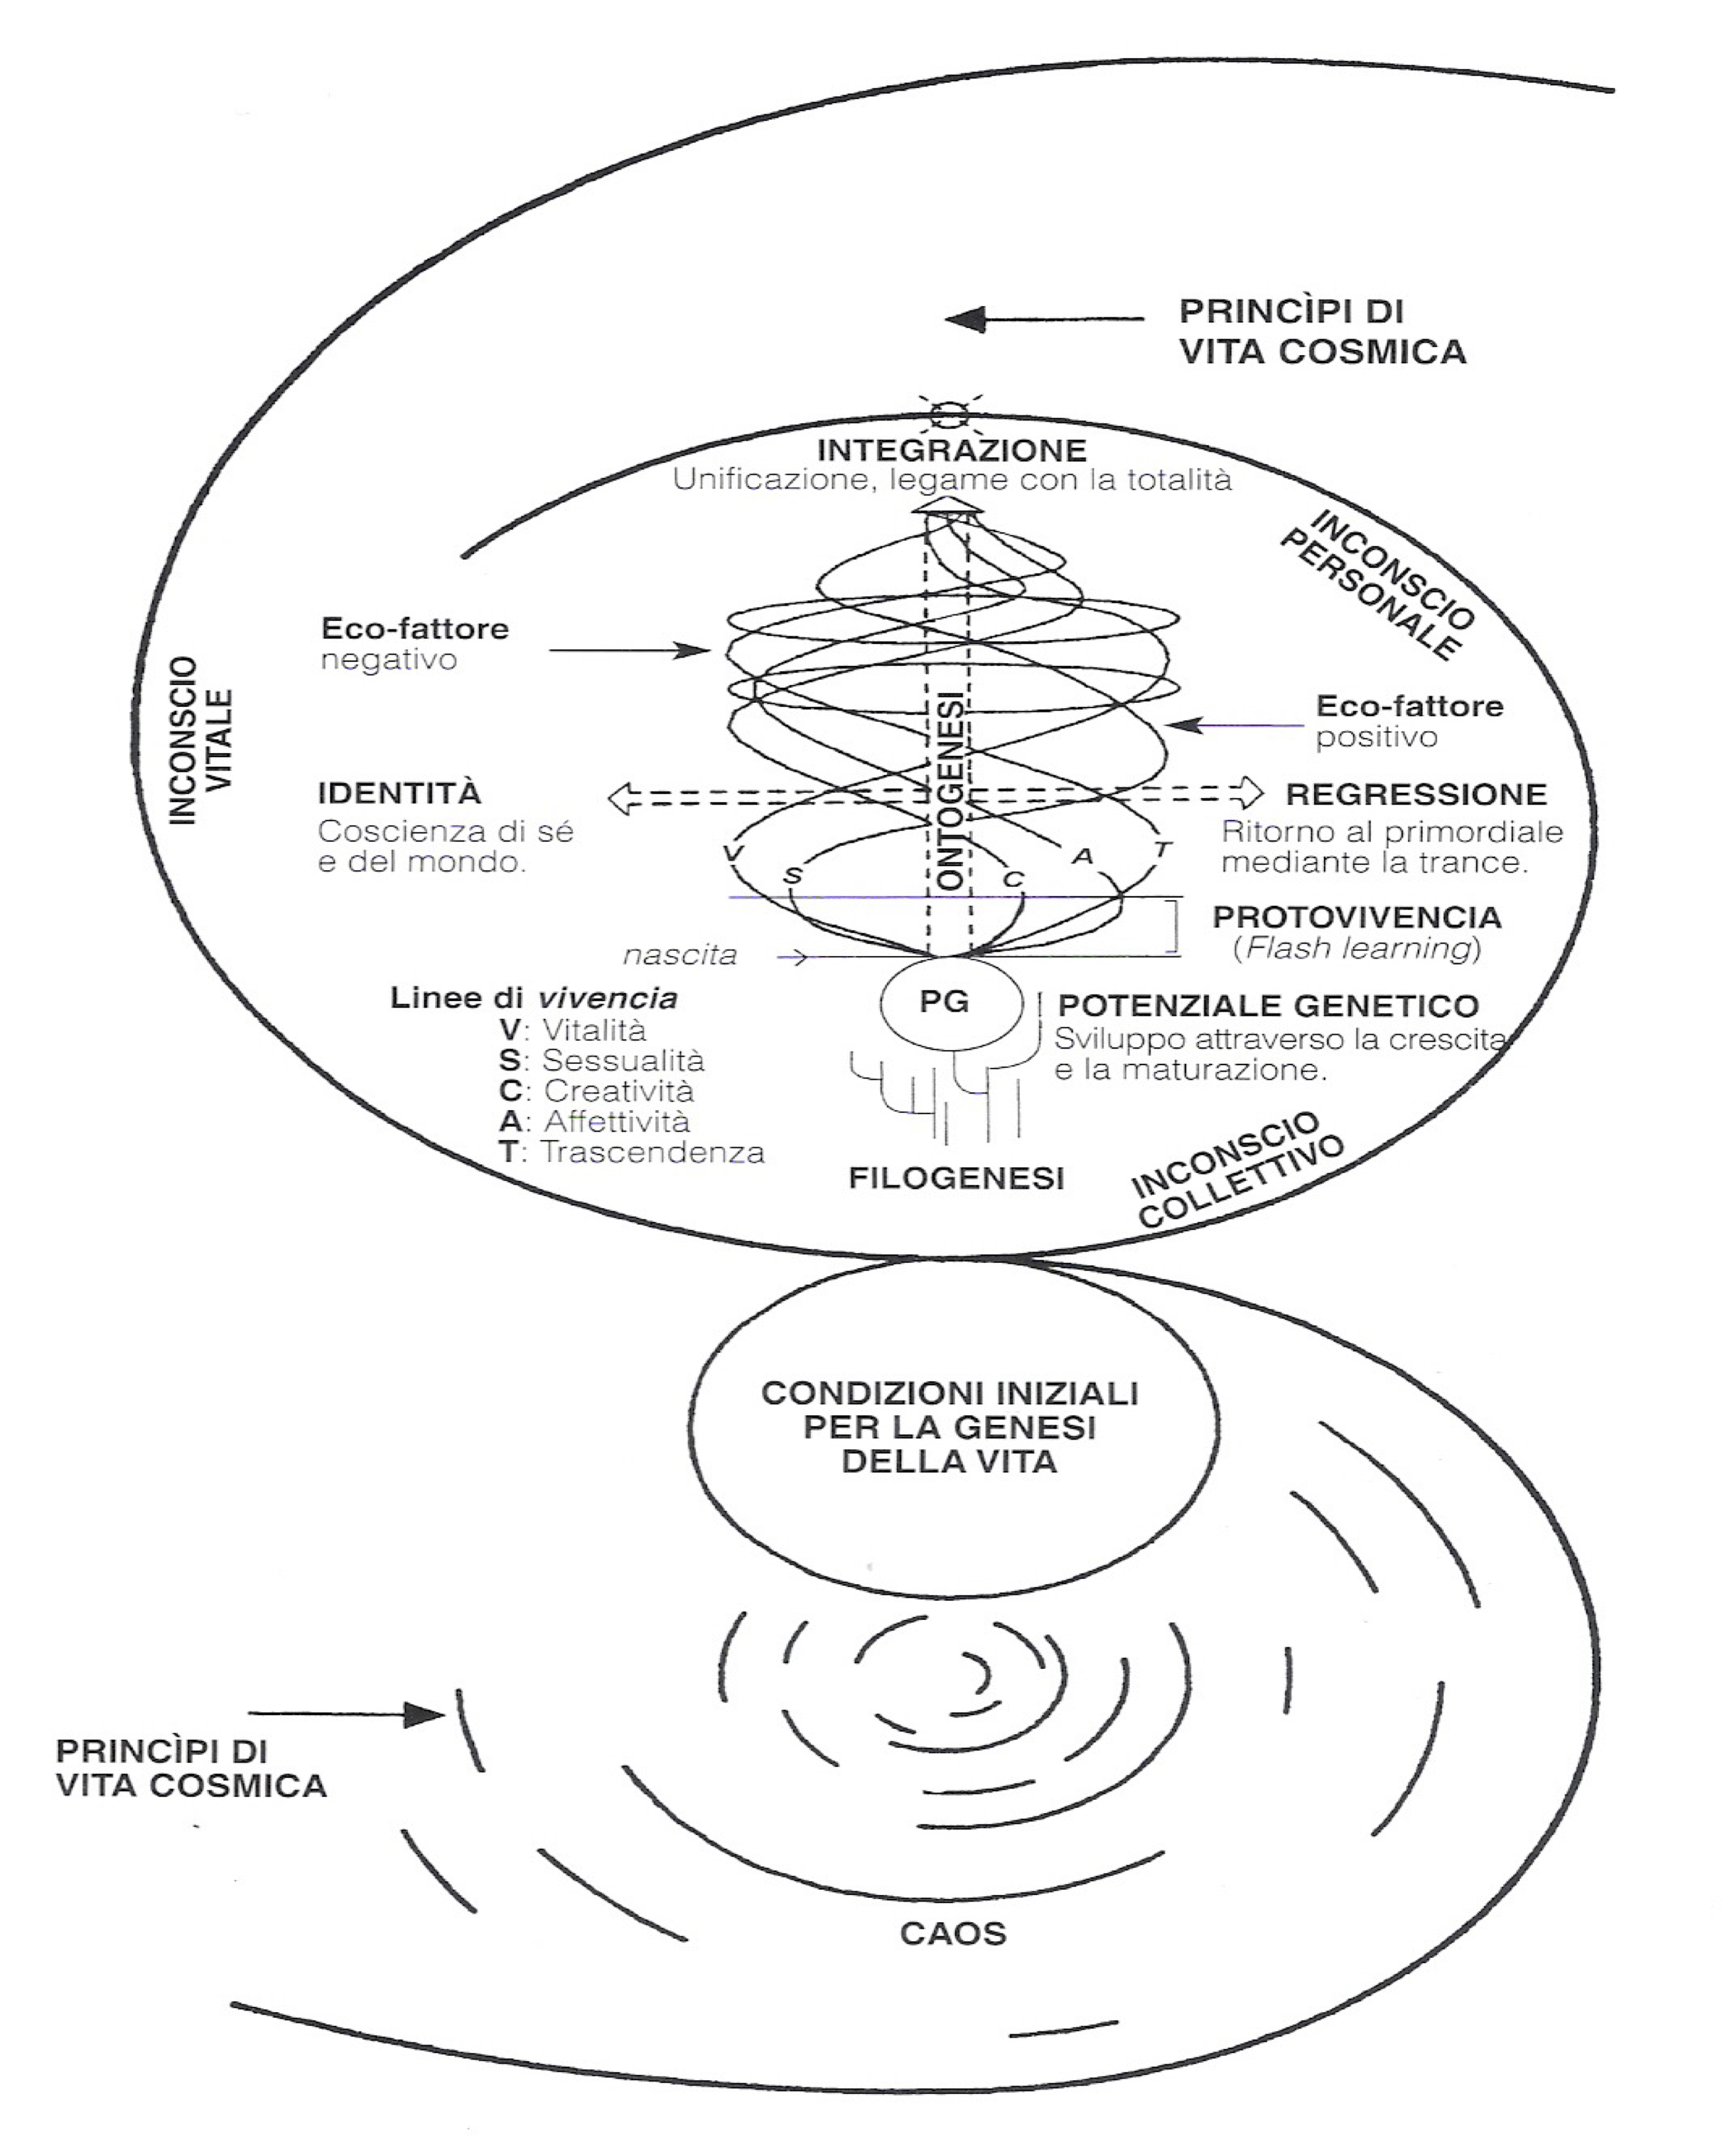
\includegraphics[width=1\linewidth]{./figs/biodanzaModel} 

}

\caption{Model of Biodanza}\label{fig:model}
\end{figure}

In this section I will first briefly introduce the biological aspects in the model of Biodanza, which is the main theme of this monograph, and next I will briefly cover the methodology of Biodanza.

\hypertarget{biological-aspects-of-biodanza}{%
\subsection{Biological aspects of biodanza}\label{biological-aspects-of-biodanza}}

The biological aspects of Biodanza can be seen as the skeleton, the vertical axis, in the model of Biodanza see Figure \ref{fig:model}. This axis consists of

\begin{enumerate}
\def\labelenumi{\arabic{enumi}.}
\tightlist
\item
  Principals of cosmic life and genesis of life
\item
  Evolution and phylogenesis
\item
  Genetic potential and ontogenesis
\end{enumerate}

Our cosmos as we know it originated out of chaos. It started with a very energy-rich state. It quickly cooled down enough for energy to be converted into mass - the majority in hydrogen and a fraction in more heavy helium nuclei. Due to the gravitational force, matter then started to cluster in nebula and eventually in stars.

In the stars all elements have been formed by nuclear fusion and with each supernova, i.e.~an explosion of a star at the end of its life, these elements/atoms are projected into space.

In space these atoms further reacted and formed more complex molecules that eventually gave rise to precursors of the biological building blocks of life.

In a remote corner of our milky way, an average galaxy, on an average planet, Earth, there originated unique conditions that made abiogenesis or the \emph{genesis of life} possible.
This was initiated by a chemical evolutionary process that gave rise to molecules with increasing complexity ultimately leading to chemistry that enabled self-replication and self-organisation and to the four essential bio-molecules of which all life is built:

\begin{itemize}
\tightlist
\item
  Lipids that enable the formation of membranes that are separating the inside of the cell from the outer world,
\item
  Carbohydrates or sugars that are used as energy sink/resource and as a backbone of many bio-molecules,
\item
  Proteins, the workhorses in our cells that facilitate the majority of chemical reactions in our cells, and
\item
  Nucleic acids, DNA and RNA, that are used to store and use our genome, i.e.~the set of genes, we inherited from our parents.
\end{itemize}

Once the first living cells emerged, they started to evolve and through evolution, they gave rise to all other living beings. This process is also referred to as phylogenesis.

We, humans, are a leaf on a small branch of the tree of life. Each of us with our own genetic potential. Through the course of our life, we develop from a fertilized egg cell to an embryo, a child, up to a full grown adult until we eventually die. During this process, which is also referred to as ontogenesis, the way how we use our genes is changed.

Indeed, at the conception we inherit the structure of our cells from our biological mothers' egg cell and our genome from our biological mother and father. At first this egg cell has access to all genes. But, as the cell divides into a clump of cells that starts to differentiate in different tissues, these more specialized cells have only access to a restricted set of genes that are essential for their function. This happens through small molecules that interact with our DNA and can switch genes on or off.
The study of how our development, behavior, and environment can cause changes that affect the way our genes are used, is also referred to as epigenetics.

Epigenetic changes are passed in cell division to the two new cells that are formed, which makes a liver cell to remain a liver cell and a brain cell to remain a brain cell upon cell division.

Also, external stimuli and eco-factors can induce epigenetic changes and can thus effectively shape how we use our genetic potential. This is exactly what we aim for with the methodology of Biodanza, which lies at the heart of the model of Biodanza.

\hypertarget{methodology-of-biodanza}{%
\subsection{Methodology of Biodanza}\label{methodology-of-biodanza}}

With Biodanza practice, we can effectively shape how our genetic potential is used. Indeed, when we experience a deep vivencia, this is accompanied by intense bodily experiences. So a Biodanza session induces physiological changes, and can thus effectively trigger the production of hormones, neurotransmitters and proteins, which originate from the expression of specific genes in our body and brain.

People who practice Biodanza for a longer period also experience that it can have a deep impact on their life and their social interactions, which is the result of rewiring in the brain.

So we can see the methodology of Biodanza as an effective tool to interact with and to impact on our body, the expression of our genes and thus on how we use our genetic potential.

The methodology of Biodanza is the central part in the model of Biodanza see Figure \ref{fig:model}, which I view as the body that is added to the skeleton of life.

\hypertarget{music-movement-and-vivencia}{%
\subsubsection{Music, Movement and Vivencia}\label{music-movement-and-vivencia}}

The most important instrument of the methodology of Biodanza is vivincia, which is evoked by means of music, movement and encounters in an affective group.

Music is a universal language and is a very powerful source of transformation. In Biodanza it has an essential function of evoking vivencia. Hence, the pieces of music used in Biodanza are very carefully chosen upon studying their emotional content, evaluating the organic effects they promote, and the type of vivencia they evoke; before they were added to the Biodanza repertoire.

Movement is another universal language that can be transformative, and, also plays a key function in evoking vivencia. Hence, movements are also very carefully chosen in Biodanza exercises. They are moderate, soft and gentle, without violence and can be executed by anyone. The sophistication of the movement comes from the meaning, emotion and feeling that is laid in it by the participant, which are of key importance for the depth of the vivencia.

So music, movement and vivencia form a gestalt. A tiny change to one component can radically alter the vivencial experience that emerges.
With the delicate choice of the sequence of Biodanza exercises, the sequence of vivencia, an overarching vivencia unfolds for the entire session.

Biodanza cannot be practiced in isolation. The encounter with each other is an essential component of movement and for generating a field that accommodates integration of oneself, with our human species and the whole.

\hypertarget{horizontal-axis-identity-vs-regression}{%
\subsubsection{Horizontal Axis: Identity vs Regression}\label{horizontal-axis-identity-vs-regression}}

Rolando has laid the foundation of his system during his career as a psychologist/researcher where he discovered the true impact of exercises that stimulate regression and identity, the horizontal axis in his system.

Each Biodanza session starts with exercises that make participants aware of their body and their identity through rhythmic activating exercises.
Then we make the bridge to more deepening exercises where we slow down our movements to lower our state of control, which evoke transcendence and integration.

\hypertarget{vertical-axis-five-lines-of-biodanza}{%
\subsubsection{Vertical Axis: Five Lines of Biodanza}\label{vertical-axis-five-lines-of-biodanza}}

Rolando structured our genetic potential in five lines: vitality, affection, creativity, sexuality and transcendence.
In a Biodanza session we typically work in two or more of these lines.

In the model the five lines are spiraling around the vertical axis of ontogenesis. Indeed, in a Biodanza session we bomb the participants with ecofactors that stimulate these five lines and that can have long-lasting effects on a genomic and physiological level.

We already get in touch with these five lines very early on in our lives, which Rolando referred to as protovivicencia. Indeed, as a baby we experience these protovivencia, e.g.~through attention, food, love, care, caressing and harmony in our environment.

During a Biodanza session we let (a subset of) the five lines pulsate by a sequence of exercises that first focus on identity and then on regression.
Exercises that strengthen identity let practitioners become more aware of themselves, the world around them and how they stand in that world. Regression on the other hand stimulates the identity to dissolve, promoting a connection with our different levels of unconsciousness.

\hypertarget{unconsciousness}{%
\subsubsection{Unconsciousness}\label{unconsciousness}}

In the periphery of methodology of Biodanza in the Model (Figure \ref{fig:model}), we find the personal unconsciousness, collective unconsciousness and vital unconsciousness.
Which is a resonance with ideas and information on ourselves, our primal instincts and archetypes, and the information that pulsates in the matrix of life, respectively.

Indeed, when a father caresses his baby, he connects with
his personal unconsciousness through the bound he experiences with his child, with the Demeter or mother archetype in his collective unconsciousness, and, with his vital unconsciousness through the physiological response he experiences through the proteins, hormones and neurotransmitters that are expressed in his cells.

So many of our actions are steered by our unconsciousness.
Through Biodanza exercises aiming for regression and transcendence we can deeply connect with these three types of unconsciousness.

When practicing Biodanza on a longer term we thus stimulate our genetic potential towards integration and connectedness with ourselves, our species and life as a whole, which Rolando referred to with the metaphor ``the cosmic human''.

\newpage

\hypertarget{aims-of-this-monograph}{%
\section{Aims of this monograph}\label{aims-of-this-monograph}}

This monograph focuses on the Biological aspects of Biodanza and originates from the module on Biological aspects of Biodanza for which I have given the theory in the School of Antwerp.

In particular, I will try to place all concepts that appear in the official learning material of the Biodanza teacher training of the Scuolatoro, the Mother school of Biodanza, in the context of the Model of Biodanza. It is my humble attempt to provide more insight in these biological aspects for Biodanza practitioners and facilitators without a formal scientific background.

This attempt consists of five parts:

\begin{enumerate}
\def\labelenumi{\arabic{enumi}.}
\item
  ``What is Life'', which gives a basic foundation and introduces important biological concepts that might provide a deeper insight in the concepts Biocentric Principle and Vital Unconciousness.
\item
  ``Principles of Cosmic Life and the Genesis of Life'', which I will try to introduce in a short narrative on the history of the universe up to the origin of life.
\item
  ``Evolution and Phylogenesis'', which tells a brief story on the history of life and how life evolved.
\item
  ``Ontogenesis'', which tries to shed some light on how our cells evolve from our origin as a fertilized egg cell up to our adult stage until we eventually die.
\item
  ``Ontogenesis and Biodanza'', a short view on how the Method of Biodanza might impact ontogenesis in our path towards integration
\end{enumerate}

\hypertarget{what-is-life}{%
\chapter{What is Life?}\label{what-is-life}}

This chapter is largely built on the work of five scientists who were very influential and who largely shaped Rolando Toro's views on the biological aspects that he incorporated in his Model for Biodanza:

\begin{itemize}
\tightlist
\item
  Erwin Schrödinger who explicitly defined life as structuring ``order-from-disorder'',
\item
  Ilia Prigogine who developed the theory for this and coined the term ``Dissipative Structures'',
\item
  Christian de Duve one of the founding fathers of biochemistry and from whom Rolando borrowed the phrase that ``Life is an obligatory manifestation of matter, written into the fabric of the universe'', and
\item
  Humberto Maturana and Francisco Varela with their concept of autopoiesis,
\end{itemize}

on which we will elaborate in the sections below. I will also link them to two core concepts of Biodanza: the Biocentric Principle and Vital Unconsciousness.

\hypertarget{schruxf6dinger-and-prigogine-a-thermodynamic-view-of-life}{%
\section{Schrödinger and Prigogine: a Thermodynamic View of Life}\label{schruxf6dinger-and-prigogine-a-thermodynamic-view-of-life}}

In his seminal lecture series: ``What Is Life? The Physical Aspect of the Living Cell'' \citet{schrodinger1944} defined life as

\begin{enumerate}
\def\labelenumi{\arabic{enumi}.}
\item
  an open system that can generate order from chaos by exploiting external energy sources,
\item
  with the capacity to transmit its own specific blueprint from generation to generation.
\end{enumerate}

Note, that in his seminal lecture series \citet{schrodinger1944} also laid out key functions of the molecule that was involved in this specific blueprint and this while DNA was not even discovered.

At first, the property that life can generate order or structure seems to contradict the second law of thermodynamics that states that: a closed system is always gearing towards maximal entropy.

Entropy can be loosely defined as a physical quantity for the level of how energy is spread out. It is thus the tendency of a closed system to evolve from a concentrated energy state to an energy state that is more spread out. This can be easily explained with an example that is well known to anyone: if you put a hot pot in a large room, the pot will cool down and the temperature in the room will slightly rise until the pot and the room have the same temperature. As a result the concentrated heat energy from the pot is nicely spread out over the entire room.

Schrödinger understood that life was not violating this second law. Indeed, by being an open system, it can interact with the environment, and by eating and breathing there has to be a way of ``concentrating order'' or maintaining a higher more concentrated energy state.

Prigogine was the first to provide the theoretical framework for a type of chemistry that is key for life \citep{prigogineStengers1984}. He realized that the chemistry of life is totally different from most chemical systems that were studied up to then. Indeed, the chemistry and processes of life are highly non-linear with many feedback loops and are far from equilibrium.

We intuitively know the latter: a living system is typically at a higher energy state than the corresponding material in a non-living state. We can simply acknowledge that as we are hotter than the room, and a crude way to estimate how long we are death is by measuring the temperature of a corpse. To maintain our higher energy state we have to keep on eating and breathing in order to stay warm, to concentrate elements in our cells and to build ordered molecules with a high chemical energy content from it.

Prigogine discovered that complex self-organizing systems can spontaneously arise if they are open and can exchange lots of energy and matter with their surroundings.
Key for it is a chaos of matter and a flow of energy through the system.
In chemical systems, and life is to a large extent chemistry, the influx of energy allows the generation of structure while producing lots of entropy by dissipation. Dissipation means that energy has been converted from one energy form to another and that it can no longer be converted back in its original form. So dissipation is irreversible, which adds the arrow of time to life. Indeed conversion of energy to heat inherently takes place in all underlying chemical reactions and these chemical reactions cannot be reversed without the addition of new energy. Hence, in the chemistry of life a large part of the concentrated energy that enters the system under the form of sunlight or chemical energy in food is spread out in less concentrated energy in the form of heat that is released by the chemical reactions that take place in our cells.
The structure that spontaneously emerges out of chaos is thus not violating the second law because of the rise in entropy by the dissipation of heat.
Prigogine therefore coined the novel term dissipative structures for such systems.

In the module of the Biodanza teacher training on the Biocentric Principle Rolando Toro often uses the term attractor. Dissipative structures typically have multiple attractors, i.e.~states, regimes, forms, shapes or structures to which they spontaneously evolve. The specific attractor to which the system is organizing itself highly depends on the initial environmental conditions.
Note, that dissipative structures are also characterized by feedback loops.
These feedback loops allow the system to remain at its current attractor upon changes in the environment.
However, some environmental stimuli are amplified by the feedback loops and can switch the dissipative structure towards another attractor and thus induce a regime switch.

Prigogine argued that chemistry in cells, cells itself, tissues, organs, organisms, populations of organisms, ecosystems and our globe can be seen as dissipative structures \citep{prigogineStengers1984}.
The fruiting body of slime molds are a compelling example of the change of the attractor of a system, see figure \ref{fig:Dictyostelium}. Dictyostelium slime molds, spend most of their lives as separate single-celled amoeba. But, upon stress one of the amoebas releases a chemical signal cAMP. Others detect this signal, and respond in two ways: the amoeba moves towards the signal and secretes more cAMP effectively boosting the signal. So the signal gets amplified by a feedback loop which eventually triggers the system to switch from their current attractor: a state of free living amoebas towards a novel attractor: their fruiting body (see e.g.~you tube movie \url{https://youtu.be/bkVhLJLG7ug}).

\begin{figure}

{\centering 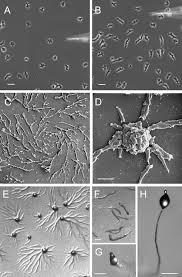
\includegraphics[width=0.6\linewidth]{./figs/Dictyostelida} 

}

\caption{Stages of Dictyostelium lifecycle. (A - B) Dictyostelium cells chemotaxing toward cAMP released from a micropipette. Cells that have not yet sensed cAMP are shown in (A). Within 1 or 2 min the cells polarize and migrate toward the source of chemoattractant (B). (C - D) Scanning electron micrograph of streaming Dictyostelium cells (C) and the formation of aggregates (D). (E) Formation of aggregation centers on an agar plate. (F) Slugs moving on an agar plate. (G) Culmination stage. (H) Fruiting body. Figure from Müller-Taubergen et al. 2012}\label{fig:Dictyostelium}
\end{figure}

\newpage

In the module of the biocentric principle it is also mentioned that we live in a dissipative zone. Indeed, our whole globe can be seen as a large dissipative structure located in our solar system, which is a dissipative zone.

\begin{enumerate}
\def\labelenumi{\arabic{enumi}.}
\item
  There is an energy source, the sun that is radiating concentrated energy in photons.
\item
  Life organised structure from the chaos of molecules on Earth by dissipating energy from the solar photons, light and UV, to heat through their organic pigments, e.g.~chlorophyll.
\item
  Animals, bacteria and fungi are secondary dissipative structures that are feeding on the concentrated chemical energy in the form of sugar and starch that is produced by plants and cyanobacteria. They again dissipate energy in the form of heat through respiration.
\item
  The heat produced by life is dissipated to water and air and this induces tertiary dissipative processes like the water cycle, wind and sea currents etc.
\item
  Eventually heat is radiated to space, which acts as an energy sink.
\end{enumerate}

Because the temperature of Earth remains roughly stable, the same amount of energy is radiated to space under the form of heat as what comes in under the form of photons from the sun. As the energy content of heat is lower and more disperse it has a higher entropy than that of the incoming sunlight.
Because almost no mass is exchanged between Earth and space, mass has to be recycled and life is inherently cyclic.

Prigogine showed that dissipative structures spontaneously emerge as soon as there is an energy source and sink, and thus an energy flow, and, a chaos of mass/chemicals available.
This is also what happened on earth. Earth exists about 4.5 billion years and a soon as there was water on Earth, life spontaneously emerged in less than 3 million years.

\hypertarget{de-duve-a-biochemical-view-of-life}{%
\section{de Duve: a Biochemical View of Life}\label{de-duve-a-biochemical-view-of-life}}

In his Book ``Life Evolving - Molecules, Mind and Meaning'', \citet{deDuve2002} gave a very simple but brilliant definition of life:

Life is

\begin{enumerate}
\def\labelenumi{\arabic{enumi}.}
\tightlist
\item
  One,
\item
  Chemistry, and
\item
  Information
\end{enumerate}

In the following sections we will explore what de Duve meant with each component in his definition.

\hypertarget{life-is-one}{%
\subsection{Life is One}\label{life-is-one}}

The first part in the definition of de Duve, ``Life is One'', has been instrumental for Rolando Toro when he coined the term ``Vital Unconsciousness''.

\hypertarget{all-living-organisms-are-built-of-cells}{%
\subsubsection{All Living Organisms are Built of Cells}\label{all-living-organisms-are-built-of-cells}}

``Life is One'' because all organisms are composed of cells.
Green algae that can perform photosynthesis are a beautiful example of unicellular organisms. They were key for the development of life on our planet by releasing oxygen in our atmosphere (Figure \ref{fig:greenAlgae}).

\begin{figure}

{\centering 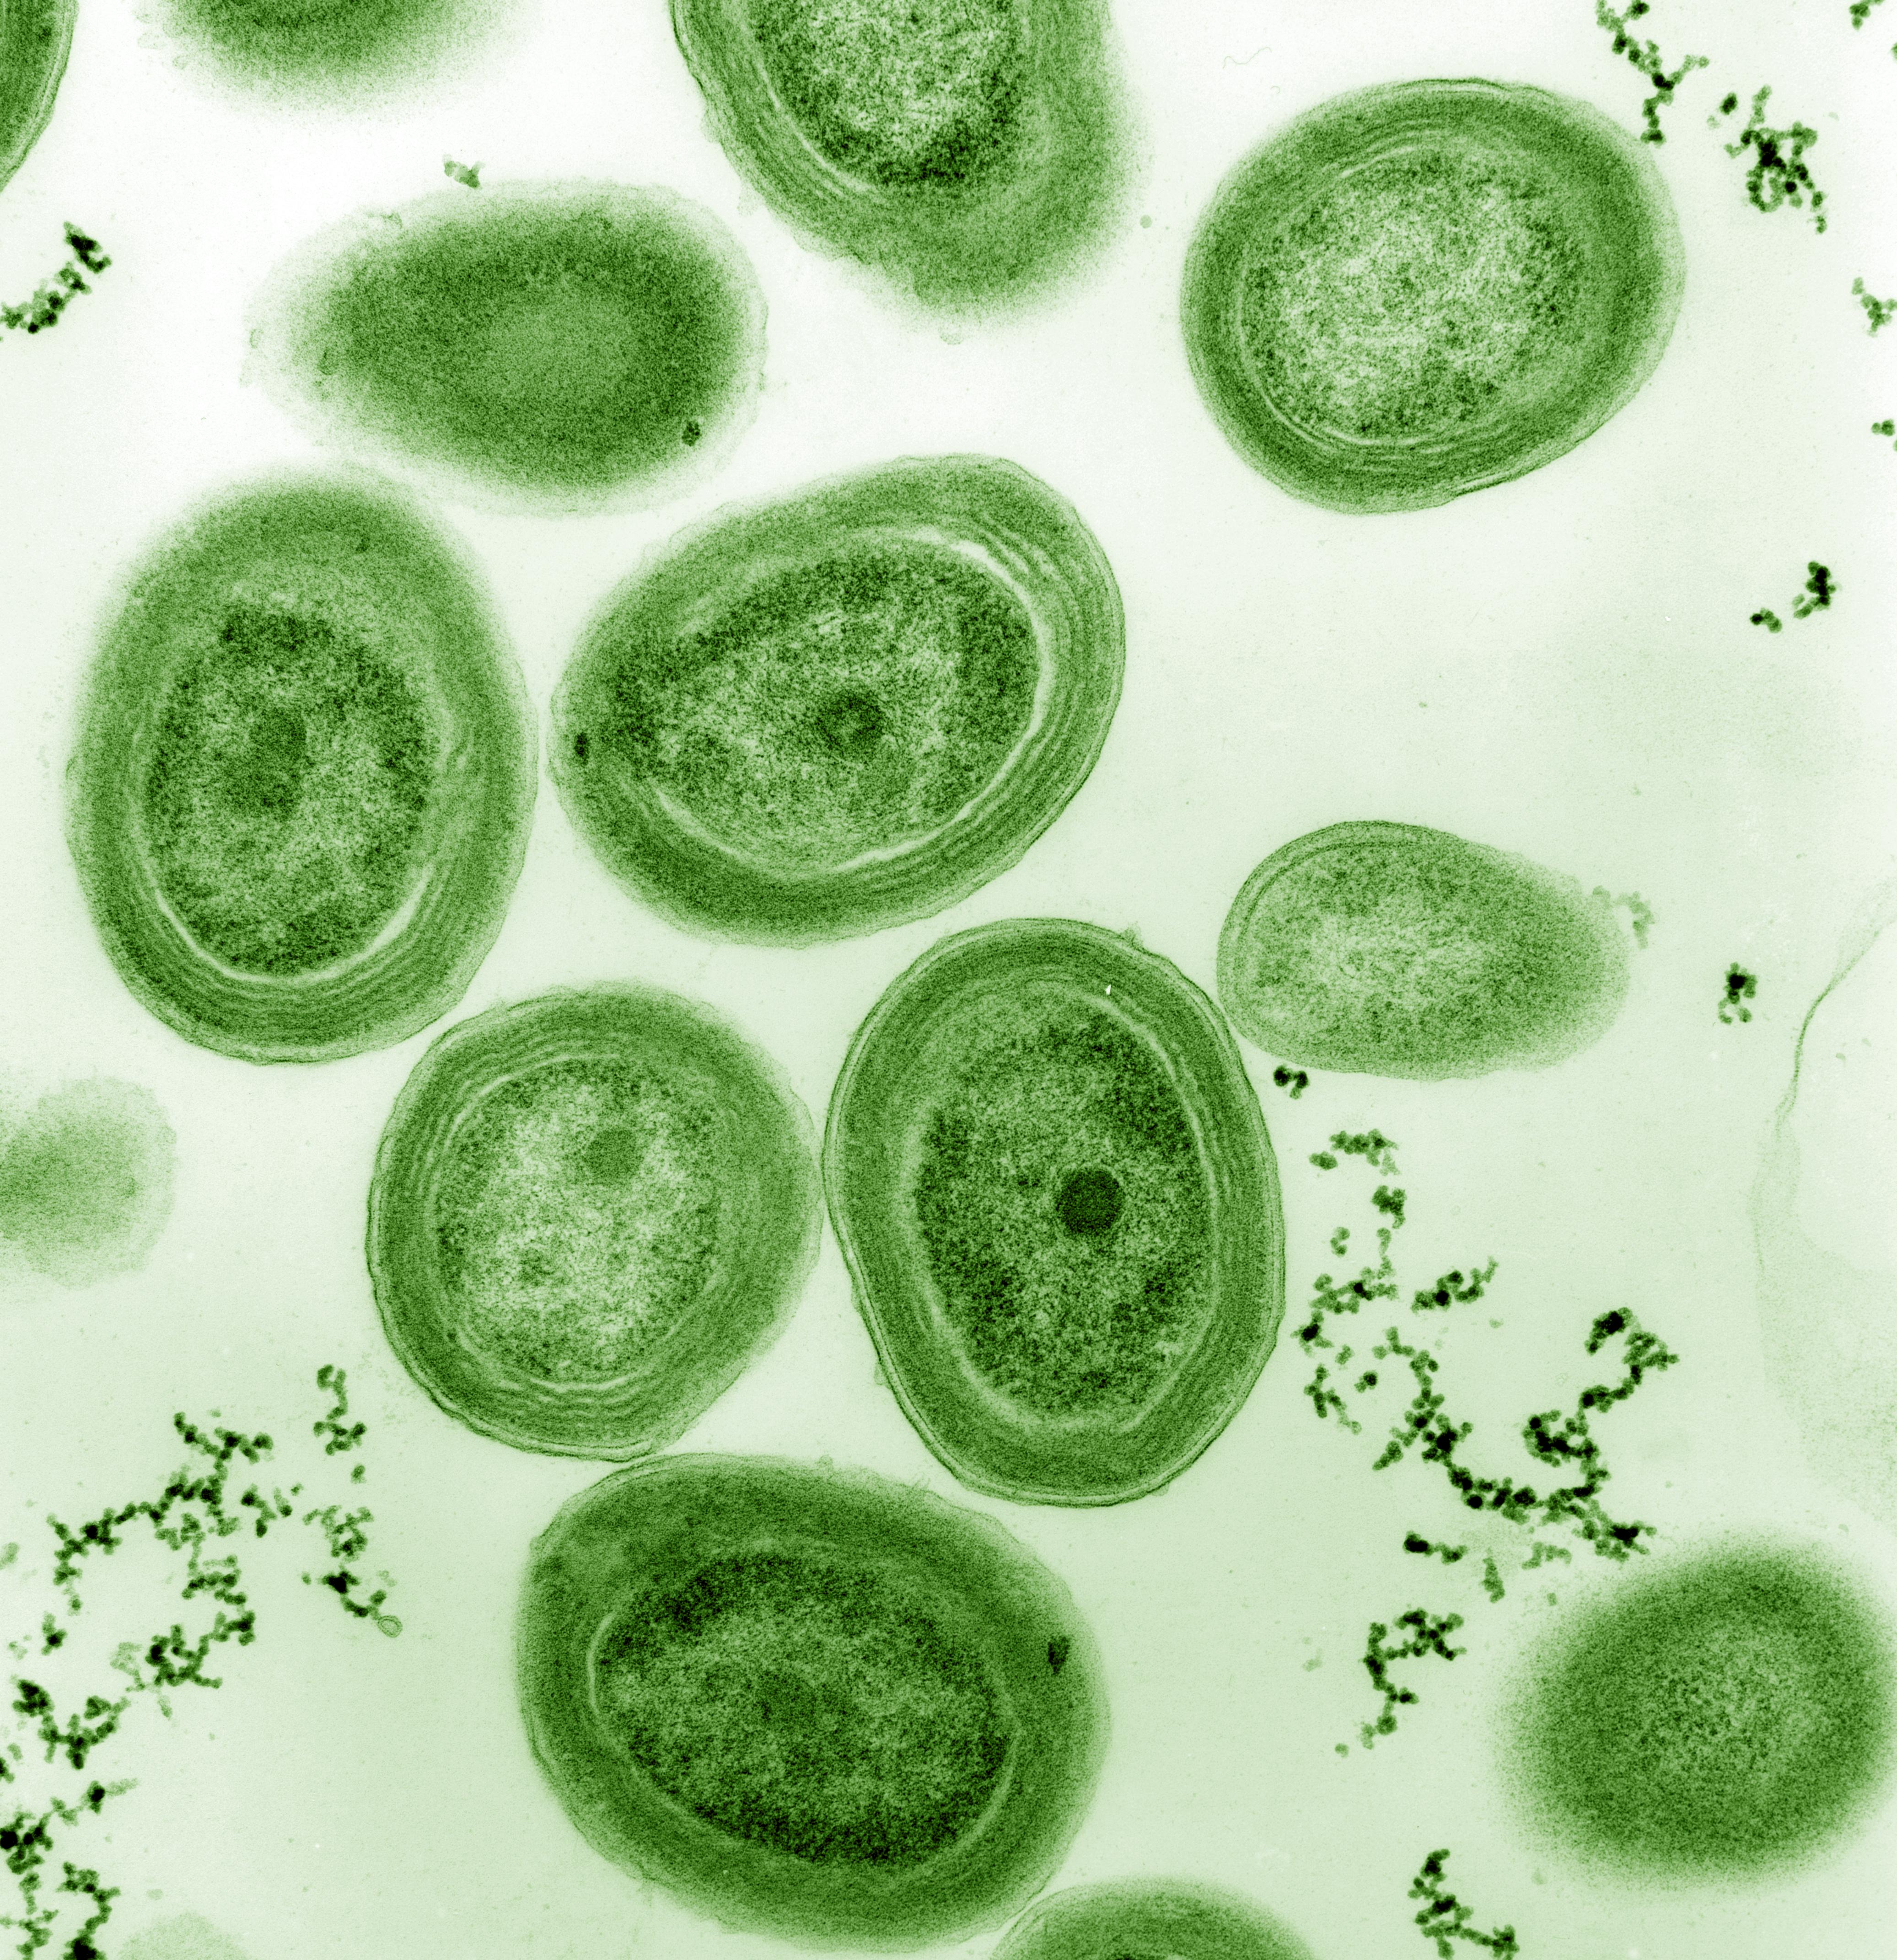
\includegraphics[width=0.3\linewidth]{./figs/Prochlorococcus_marinus} 

}

\caption{Cyanobacteria, unicellullar organisms that can perform photosynthesis. They were key in the development of life and radically changed Earth by releasing oxygen to our atmosphere (Source: Chisholm Lab, Wikipedia)}\label{fig:greenAlgae}
\end{figure}

A vital component of a cell is its membrane that is separating them from their environment while enabling them to interact with it and to concentrate chemicals inside the cell.

Multicellular organisms are composed of multiple cells. The cells are organised in

\begin{itemize}
\tightlist
\item
  tissues, e.g.~spongy tissue in our bones or epithelium cells of our stomach,
\item
  organs, e.g.~bones or our stomach,
\item
  organ systems, e.g.~skeleton or digestive system, etc.
\item
  organism
\end{itemize}

Figure \ref{fig:multiCellular} also shows how multicellular organisms are further organised in

\begin{itemize}
\tightlist
\item
  populations of organisms
\item
  ecosystems, and
\item
  eventually our entire Biosphere
\end{itemize}

So ``Life is One'' because all living organisms consist of cells, and as they are organised in large networks that work together at cellular, tissue, organ, organ systems, organism, population, ecosystem, up to the Biosphere level.

\begin{figure}

{\centering 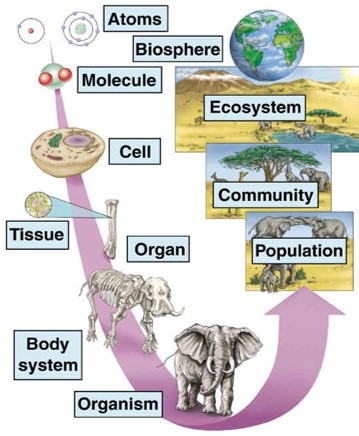
\includegraphics[width=0.3\linewidth]{./figs/organisationMulticellular} 

}

\caption{Multicellular organisms and biological organisation (Source: mrssmithsbiology)}\label{fig:multiCellular}
\end{figure}

\hypertarget{last-universal-common-ancestor}{%
\subsubsection{Last Universal Common Ancestor}\label{last-universal-common-ancestor}}

``Life is One'' because all species evolved from the same ancestral population of cells.
This is also referred to as the Last Universal Common Ancestor (LUCA). It is nicely indicated by the tree of life in Figure \ref{fig:treeOfLife}, which is one of the most important organizing principles in biology. It shows the evolutionary relationships among different organisms and that all living beings eventually can be traced back to LUCA who is located at the root of the tree. Note, that the animal kingdom to which we belong is only a small branch in the tree.

\begin{figure}

{\centering 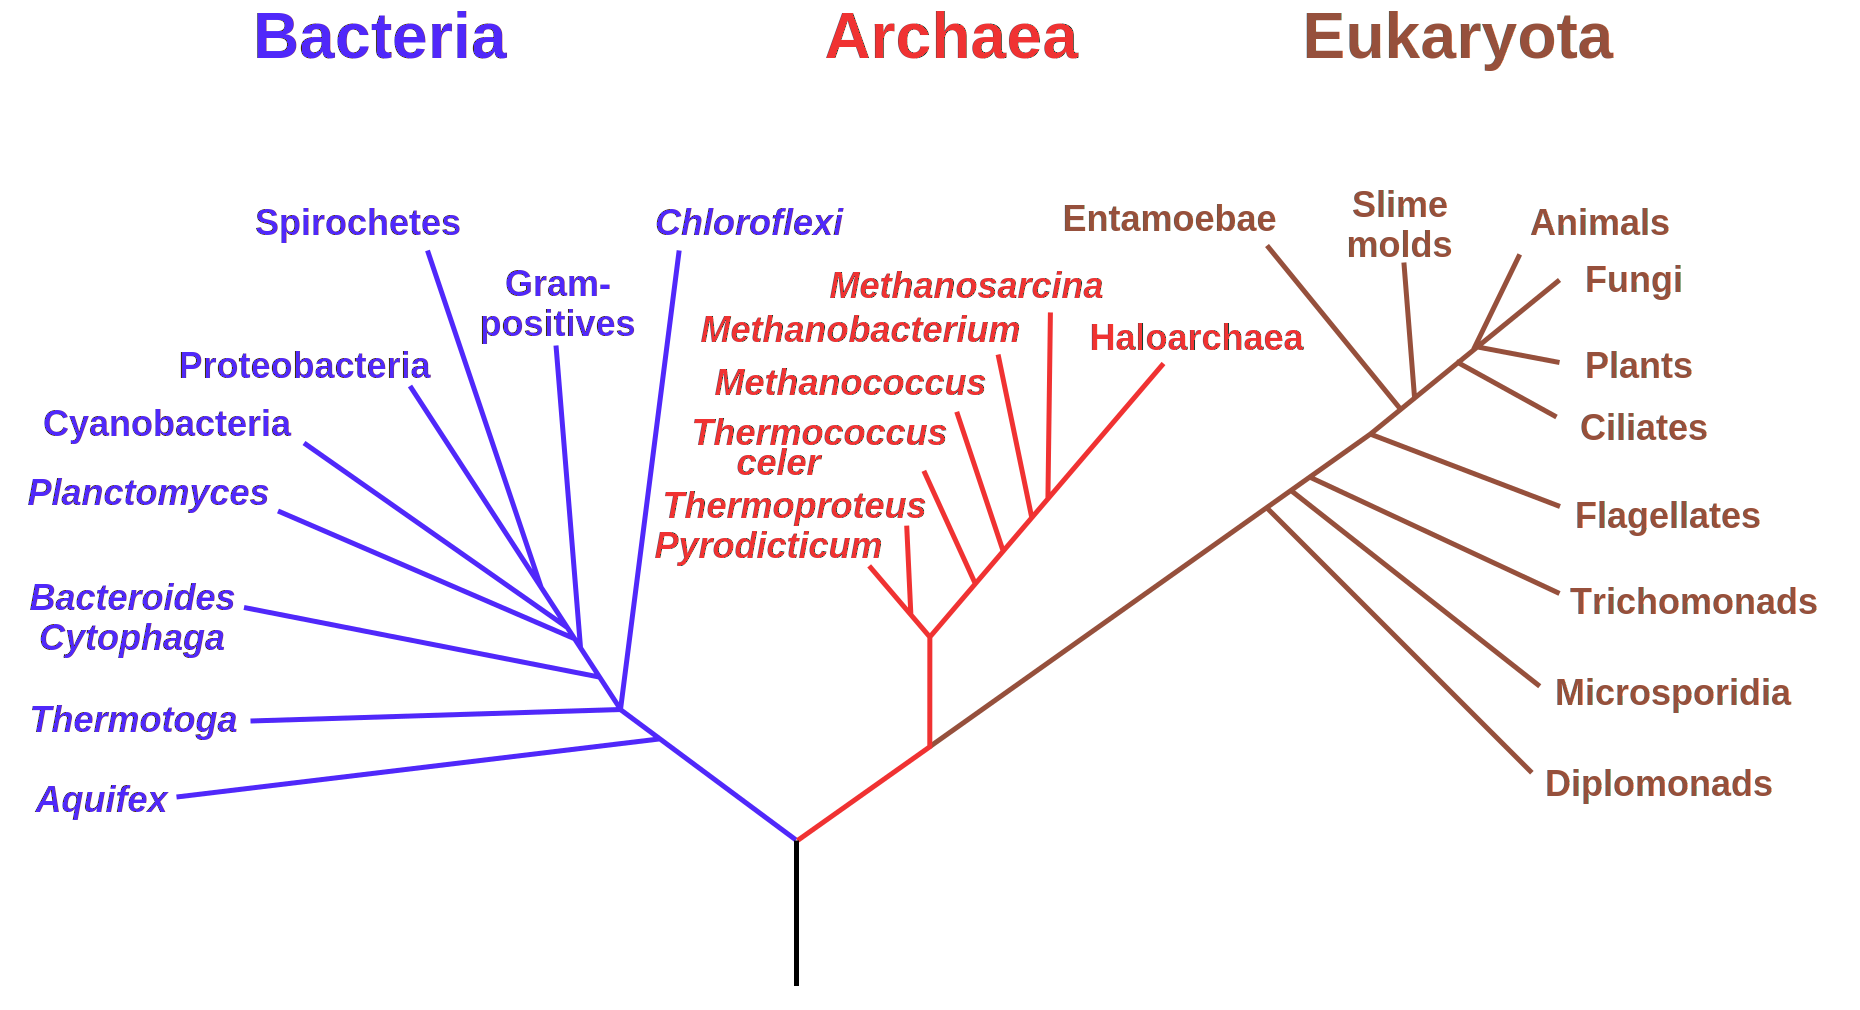
\includegraphics[width=0.8\linewidth]{./figs/Phylogenetic_tree} 

}

\caption{The tree of life is one of the most important organizing principles in biology. It shows the evolutionary relationships among different organisms and also that all living beings eventually can be traced back to the last universal common ancestor (LUCA), who is located at the root of the tree (Source: Wikipedia)}\label{fig:treeOfLife}
\end{figure}

\newpage

\hypertarget{sectionEnergyCoin}{%
\subsubsection{Energy coin}\label{sectionEnergyCoin}}

``Life is One'' because all living organisms use the same ``energy coin'', the ATP-ADP system, to store and reuse energy.
Adinosine-triphosphate (ATP) consists of a ribose sugar with 3 phosphate groups and a base adinine.
Splitting a phosphate group from adinosine-triphosphate (ATP) results in adinosine-diphosphate (ADP), a free phosphate group and energy.
The other way around, energy can be stored as chemical energy by binding a phosphate group to ADP.



\begin{figure}

{\centering 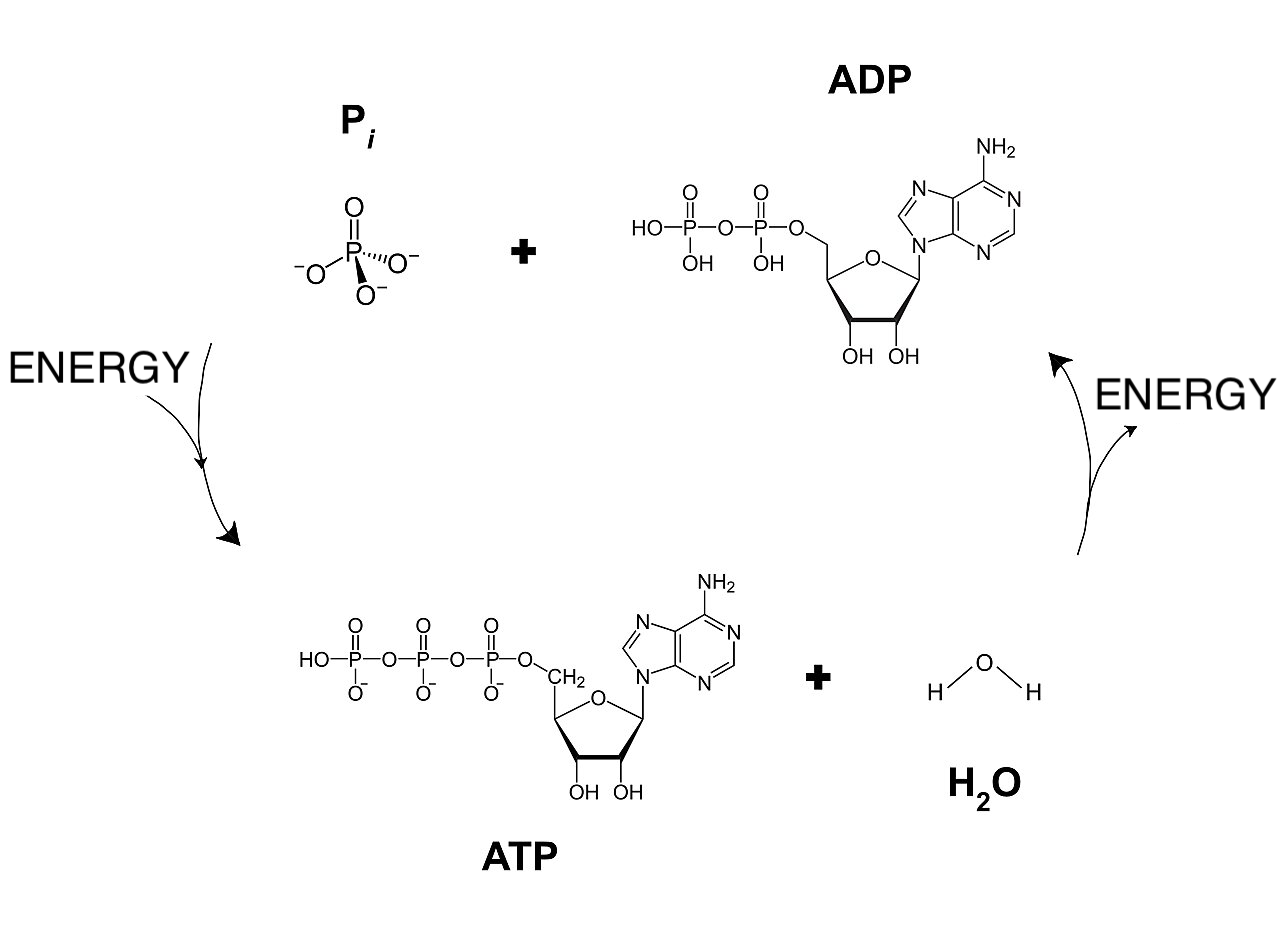
\includegraphics[width=0.7\linewidth]{./figs/ATP-ADP} 

}

\caption{Our energy coin ATP-ADP. Adinosine-triphosphate (ATP) consists of a base adinine, a ribose sugar and 3 phosphate groups. Splitting a phosphate group from adinosine-triphosphate (ATP) by a reaction with water (H\(_2\)O) results in adinosine-diphosphate (ADP), a free phosphate group and energy (Source: Adapted from Wikipedia)}\label{fig:atp-adp}
\end{figure}

Note, that ATP is also used to build RNA. Indeed, ATP is incorporated in RNA upon splitting two phosphate groups. The resulting AMP (adinosine monophosphate) is one of the building blocks of RNA. So there is a close link between energy and genetic information!

\hypertarget{building-blocks-of-life}{%
\subsubsection{Building Blocks of Life}\label{building-blocks-of-life}}

``Life is One'' because all living organisms are composed of the same basic bio-molecules and we all know more than we think about them because we are what we eat!\\
Almost all molecules of living organisms are composed of

\begin{enumerate}
\def\labelenumi{\arabic{enumi}.}
\tightlist
\item
  Lipids, oil and fats, for storage and as building blocks for membranes,
\item
  Carbohydrates, sugars, for storing energy and as a backbone of large bio-molecules,
\item
  Amino acids, the building blocks of proteins, which are the workhorses of a cell, and
\item
  Nucleic Acids, building blocks of RNA and DNA, which are used to store and use the genetic information we inherit from our parents.
\end{enumerate}

\hypertarget{lipids}{%
\paragraph{Lipids}\label{lipids}}

\begin{figure}

{\centering 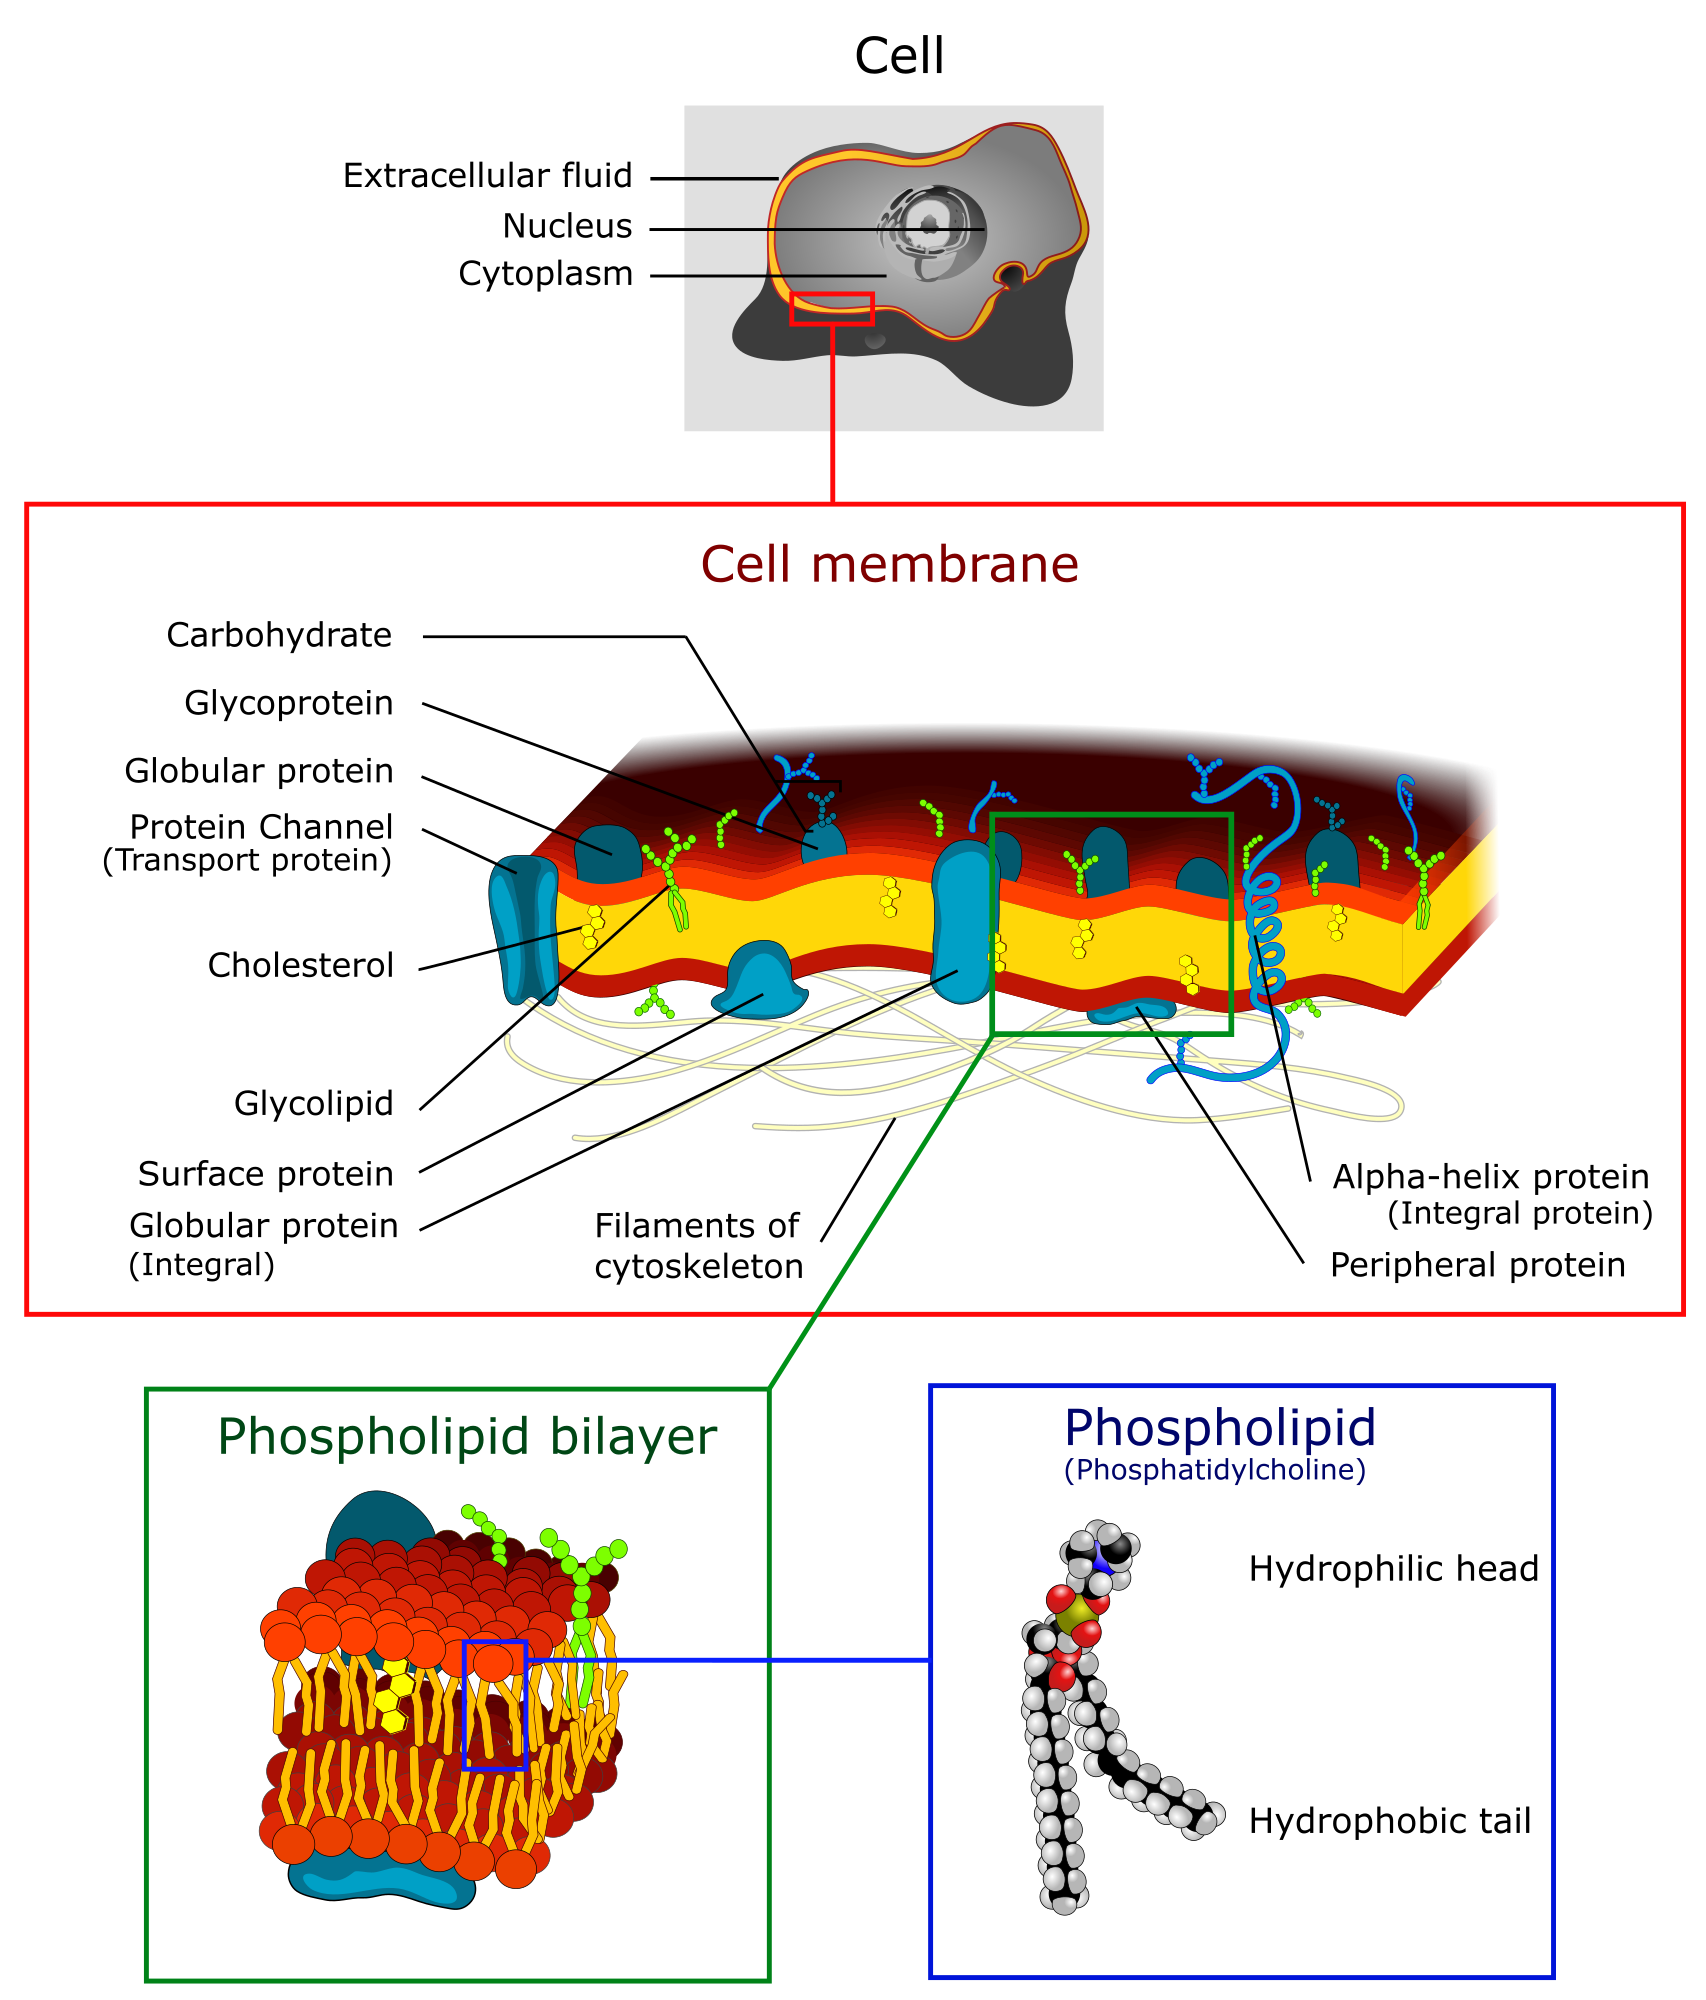
\includegraphics[width=0.8\linewidth]{./figs/Cell_membrane_detailed_diagram_4} 

}

\caption{Phospho-lipids have a very important role in life as they form membranes. Phospholipids have a hydrophilic head that likes to mix with water and long hydrophobic tails that do not mix with water. They sponteneously gives rise to bilayers in aqueous solutions similar to the structure seen in membranes. Membranes are the boundaries of the cell and they allow passivie diffusion of small molecules through their bilayer. Larger molecules can be actively exchanged with the environment through membrane proteins (Source: Doug Hatfield, Wikipedia)}\label{fig:lipids}
\end{figure}

Lipids, fats and oils, are used for storage. However, an important class of lipids, the phospholipids, make up membranes of cells and unicellular compartments called organelles see Figure \ref{fig:lipids}. Indeed phospholipids have a polar head that likes to be in water and a long apolar tail that does not mix with water. Therefore bilayers of phospholipid molecules are spontaneously formed in aqueous solutions.

Membranes provide the basis for concentrating specific molecules in (compartments of) living cells. This forms a disequilibrium of chemical molecules that can perform work as the concentration gradient spontaneously dissipates toward its equilibrium value. So phospholipids are key for creating the boundary conditions necessary for cellular organization.

\hypertarget{carbohydrates}{%
\paragraph{Carbohydrates}\label{carbohydrates}}

Carbohydrates are important bio-molecules that are used for storage, energy and structure (Figure \ref{fig:carbohydrates}).

\begin{figure}

{\centering 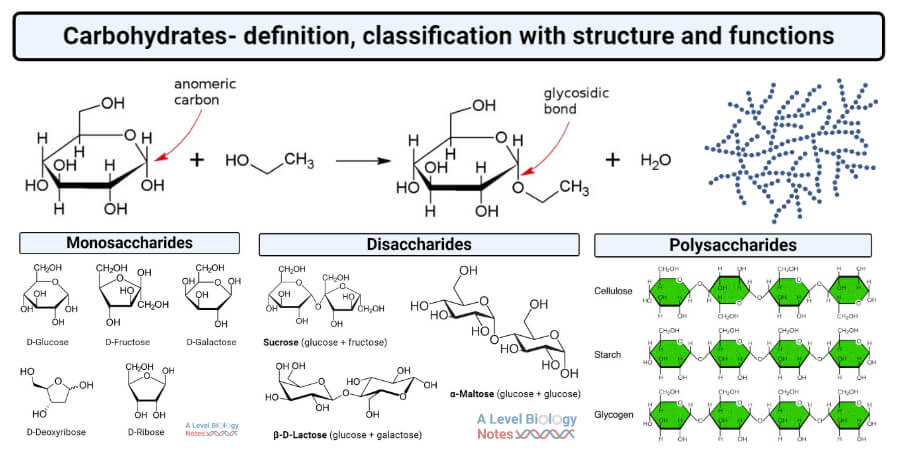
\includegraphics[width=1\linewidth]{./figs/Carbohydrates-definition-classification-with-structure-and-functions} 

}

\caption{Carbohydrates perform the important functions of storage, energy source and structure. They can be organised in biopolymers, long chains of carbohydrate molecules that are bound together. The polysaccharides starch and glycogen for instance are used to store energy by plant and animal cells, respectively. Cellulose, on the other hand, is a polysaccharide that gives plants structure. Deoxyribose and ribose are important carbohydrates that form the backbone of the biopolymers DNA and RNA, respectively. (Source: thebiologynotes.com)}\label{fig:carbohydrates}
\end{figure}

\begin{itemize}
\tightlist
\item
  Storage: glucose is stored inside animal cells using glycogen, a polymer of thousands of glucose molecules that are bound to each-other. Plants use a similar molecule, starch.
\item
  Energy source: specific proteins can split glycogen and starch into glucose that is subsequently metabolized for energy.
\item
  Structure: carbohydrates form the backbone of many bio-molecules, e.g.~long chains of desoxyribose and ribose act as the backbone of the bio-polymers DNA and RNA, respectively; and glucose is the backbone of cellulose, which give plants structure.
\end{itemize}

\hypertarget{amino-acids}{%
\paragraph{Amino Acids}\label{amino-acids}}

Amino acids by themselves are simple molecules (Figure \ref{fig:aminoAcids}).
Although hundreds of amino acids exist in nature, life is using only 20 of them and it is combining them in long molecules, polymers, which are referred to as proteins.
Proteins are hetero-polymers, consisting of the 20 amino acids that are arranged in long sequences that differ from protein to protein.
So unlike starch, that only consists of glucose molecules, proteins are capable of carrying information.



\begin{figure}

{\centering 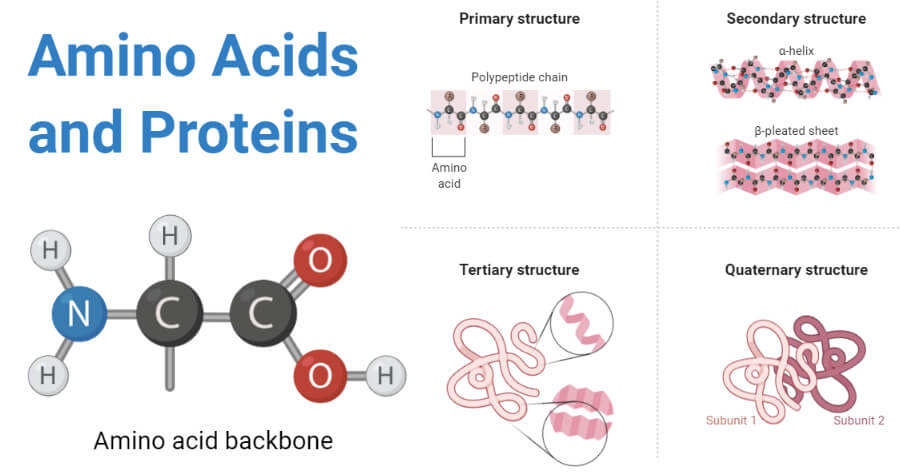
\includegraphics[width=1\linewidth]{./figs/Amino-acids-and-Proteins} 

}

\caption{Amino acids are simple molecules. They can be combined in long molecules, polymers, also known as proteins. Their long chain of amino acids spontaneously folds into a complex 3D structure from which their biological function emerges (Source: thebiologynotes.com)}\label{fig:aminoAcids}
\end{figure}

The crux of proteins is that their long chain of amino acids spontaneously folds into a complex 3D structure, which is determined by the properties and the specific sequence of its amino acids. From their complex and specific 3D structure their biological function emerges.

Indeed, many proteins work as a ``lock'' in which specific (bio)molecules fit as a ``key''. This enables proteins to bring molecules close together and to promote chemical reactions without being consumed. This process is also referred to as catalysis and proteins that perform catalysis are called enzymes, see Figure \ref{fig:enzyme}.

\begin{figure}

{\centering 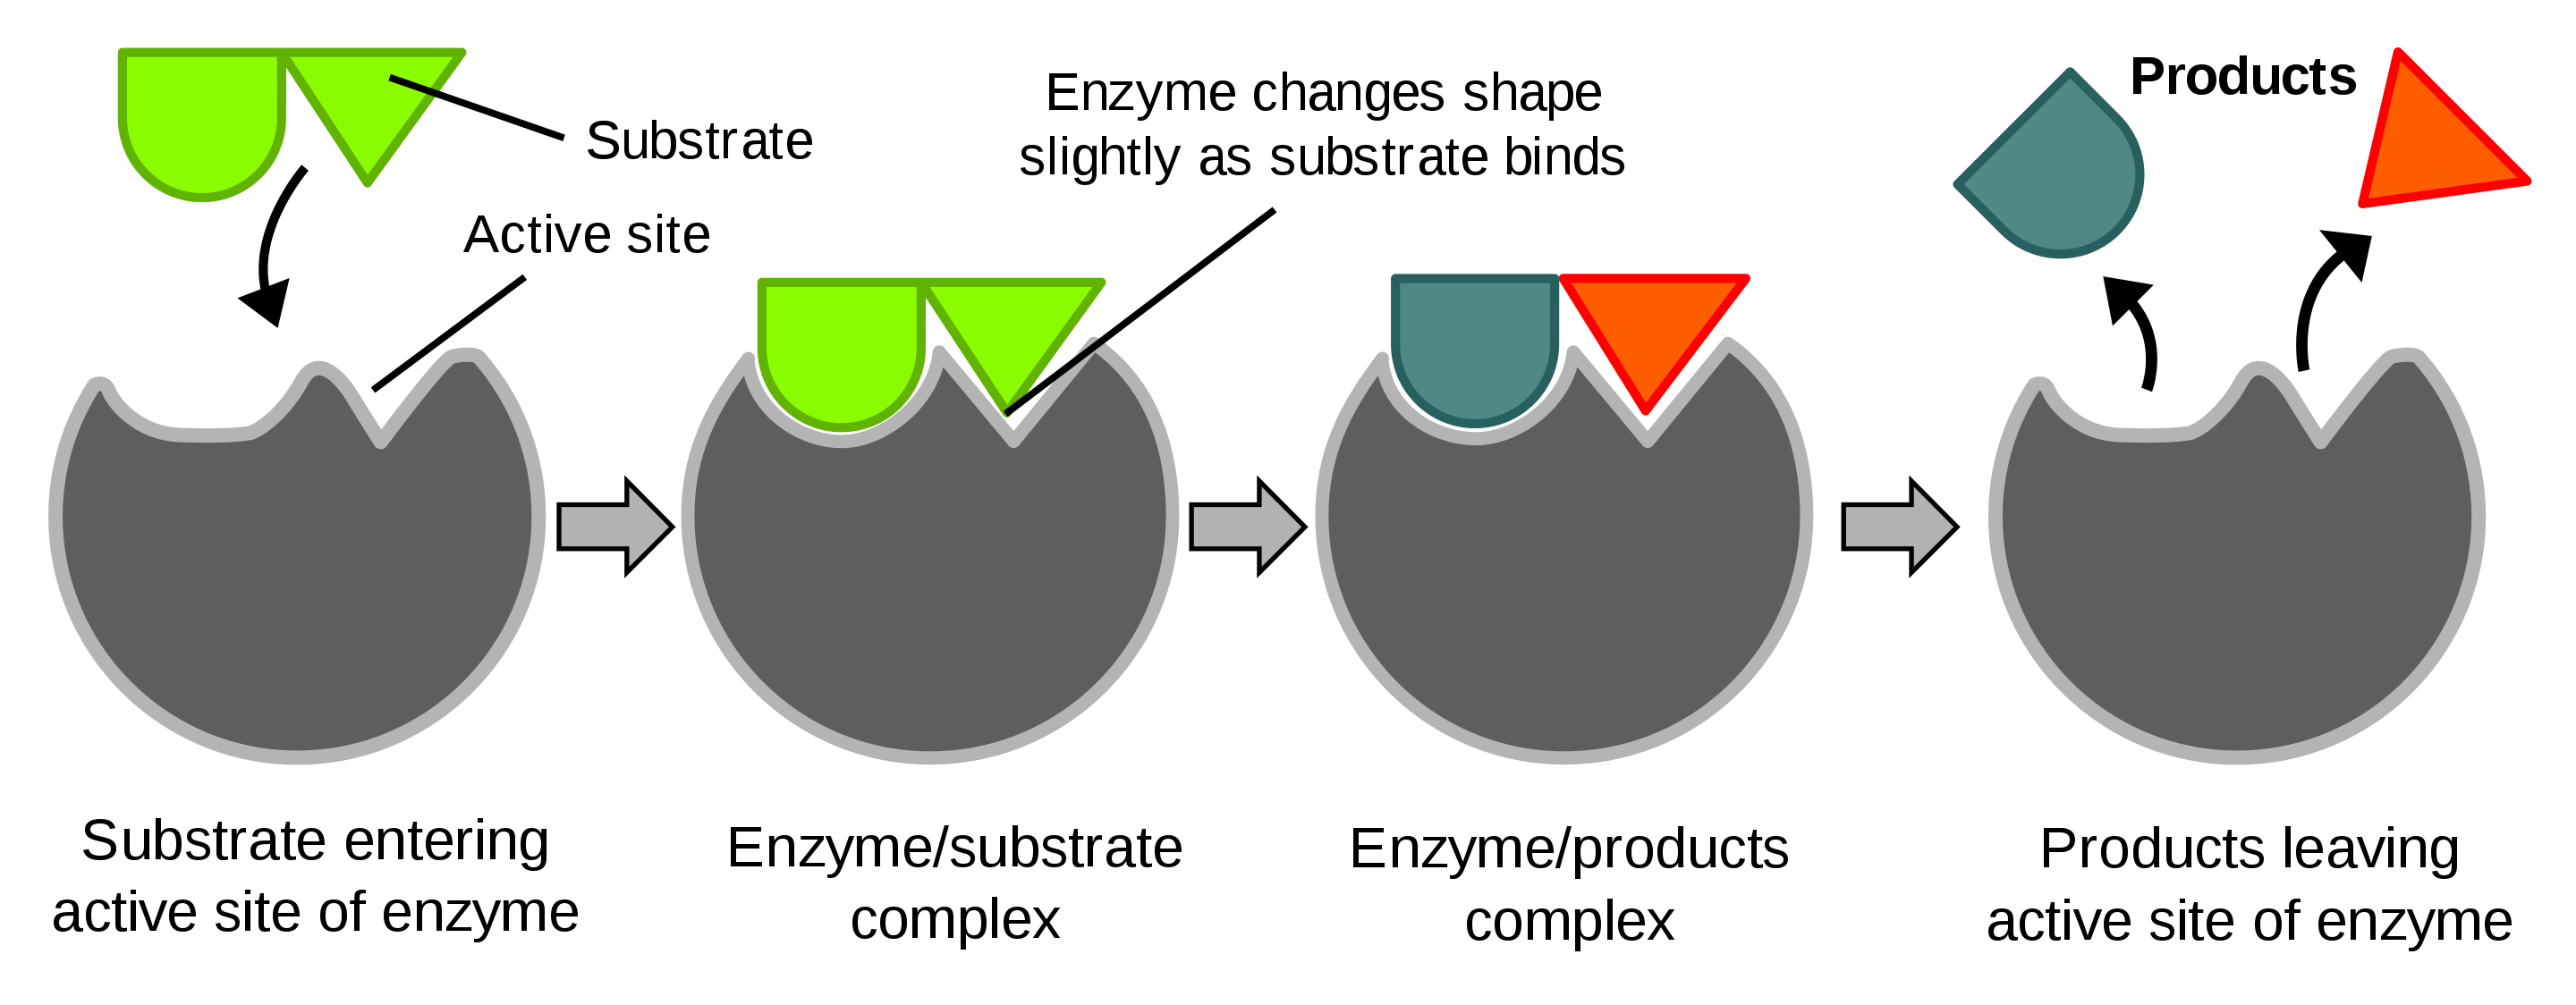
\includegraphics[width=0.5\linewidth]{./figs/EnzymePadlockKey} 

}

\caption{Diagram of enzyme action (Source: Wikipedia)}\label{fig:enzyme}
\end{figure}

Proteins are the main workhorses of the cell and they are important for moving food, digesting food, copying DNA, for giving the cell structure, affecting the rates at which other proteins work, etc\ldots{}

\hypertarget{nucleic-acids}{%
\paragraph{Nucleic Acids}\label{nucleic-acids}}

Nucleic acids are build of nucleotides.
Each nucleotide is composed of one of four nitrogen-containing nucleobases, which carry the information

\begin{enumerate}
\def\labelenumi{\arabic{enumi}.}
\tightlist
\item
  cytosine {[}C{]},
\item
  guanine {[}G{]},
\item
  adenine {[}A{]} or
\item
  thymine {[}T{]} (DNA) or uracil {[}U{]} (RNA) ,
\end{enumerate}

a phosphate group and a sugar, i.e.~ribose in ribonucleic acid (RNA, Figure \ref{fig:RNA}) and deoxyribose in deoxyribonucleic acid (DNA, Figure \ref{fig:DNA}).

These nucleotides are the building blocks that are combined in long polymers: RNA and DNA.
DNA and RNA are hetero-polymers and the nucleotides conceptually can be combined in any order.
So they can contain information.
Indeed, they are key to store and use the genetic information we inherit from our parents.

DNA typically occurs as a double strand, where C and G, and, A and T hybridize to each other using respectively three and two hydrogen bridges to form the iconic double stranded helix structure, see Figure \ref{fig:DNA}.

There is a general consensus that life probably began by using RNA as information carrier.
DNA, however, is much more stable and lasts longer in water than RNA. Therefore, DNA probably emerged later and is now used to store the genetic information in most organisms.

Life is also one because we share the same genetic code, but we refer to Section \ref{lifeInformation} ``Life is Information'' for more details.

\begin{figure}

{\centering 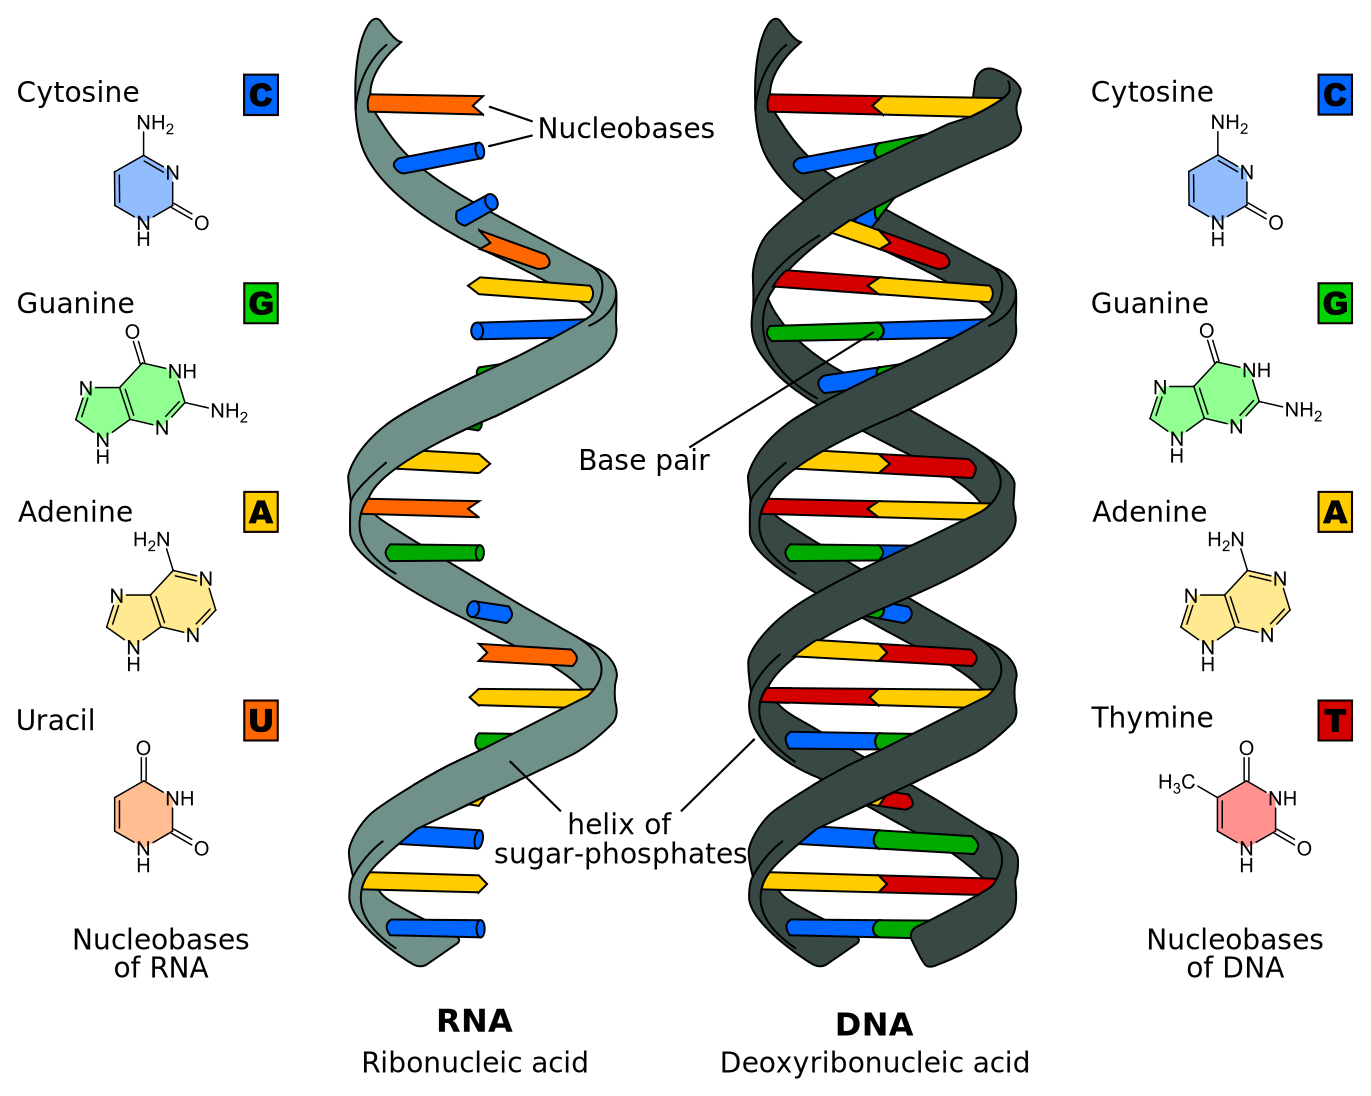
\includegraphics[width=0.5\linewidth]{./figs/Difference_DNA_RNA-EN} 

}

\caption{Nucleic acid: RNA (left) and DNA (right). RNA appears typically in a single strand and DNA as a double stranded molecule (Source: Wikipedia)}\label{fig:RNAvsDNA}
\end{figure}

\begin{figure}

{\centering 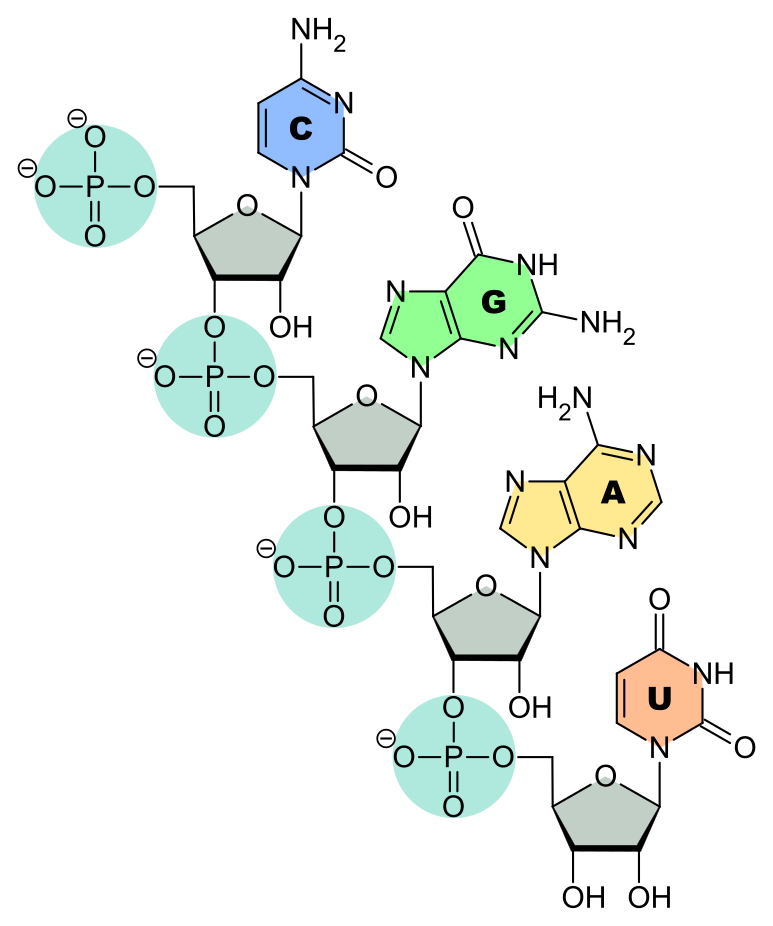
\includegraphics[width=0.5\linewidth]{./figs/RNA-Nucleobases} 

}

\caption{RNA is a polymeric molecule with various biological roles in coding, decoding, regulation and expression of genes. RNA consists of a chain of nucleotides. Each nucleotide is build from a ribose sugar that forms the backbone of the RNA  polymer, a phosphate group that is used to connect the ribose sugar molecules and a base adenine (A), cytosine (C), guanine (G) or uracil (U) that are the carriers of information. The bases can form hydrogen bonds between cytosine and guanine, between adenine and uracil, and, between adenine and thymine (a base from DNA) (Source: Adapted from Wikipedia)}\label{fig:RNA}
\end{figure}
\begin{figure}

{\centering 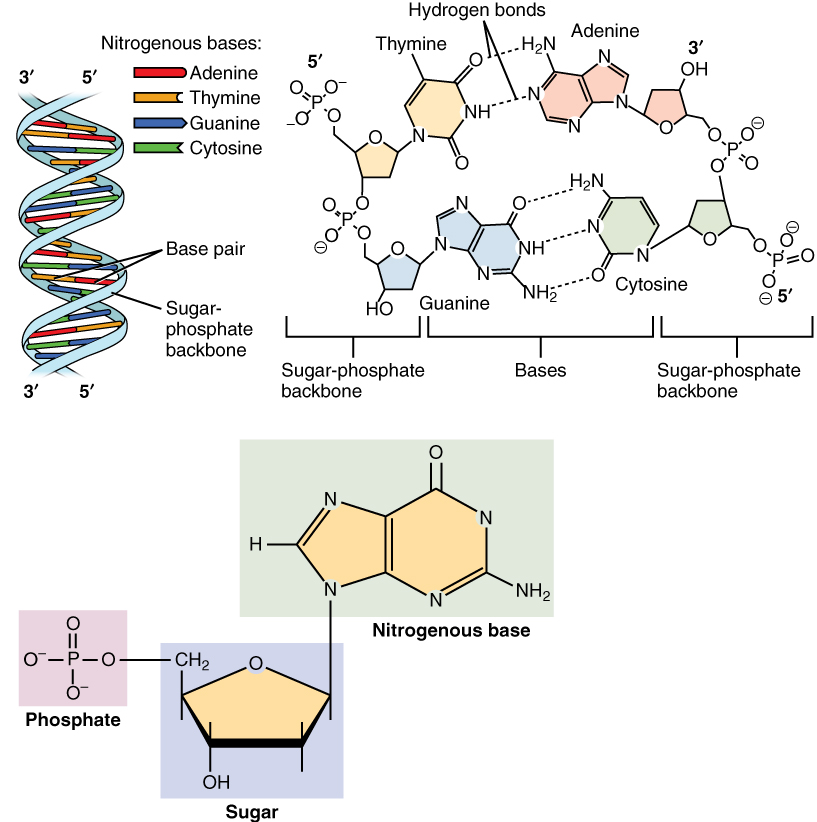
\includegraphics[width=0.5\linewidth]{./figs/DNA_Nucleotides} 

}

\caption{DNA is a polymer composed of two polynucleotide chains that coil around each other to form a double helix carrying genetic instructions for the development, functioning, growth and reproduction of all known organisms and many viruses. Each DNA single strand consists of a chain of nucleotides. Each nucleotide is build from a deoxyribose sugar that forms the backbone of the DNA  polymer, a phosphate group that is used to connect the deoxyribose sugar molecules and a base adenine (A), cytosine (C), guanine (G) or thymine (T) that are the carriers of information. The bases form hydrogen bonds between cytosine and guanine, and, adenine and thymine to assemble single stranded DNA in double stranded DNA. (Source: Wikipedia)}\label{fig:DNA}
\end{figure}

\newpage

\hypertarget{life-is-chemistry}{%
\subsection{Life is Chemistry}\label{life-is-chemistry}}

``Life is Chemistry'' because a cell consists of a network of chemical reactions that are connected to each other. Many feedback loops exist in this chemistry making it largely nonlinear. The feedback loops enables a cell to maintain in its regime or to switch from regime or attractor upon external and/or internal stimuli. An overview of most reactions in a living cell is given in Figure \ref{fig:chemicalReactionsCell}. You can zoom in on this map on \url{http://biochemical-pathways.com/\#/map/1}.

\begin{figure}

{\centering 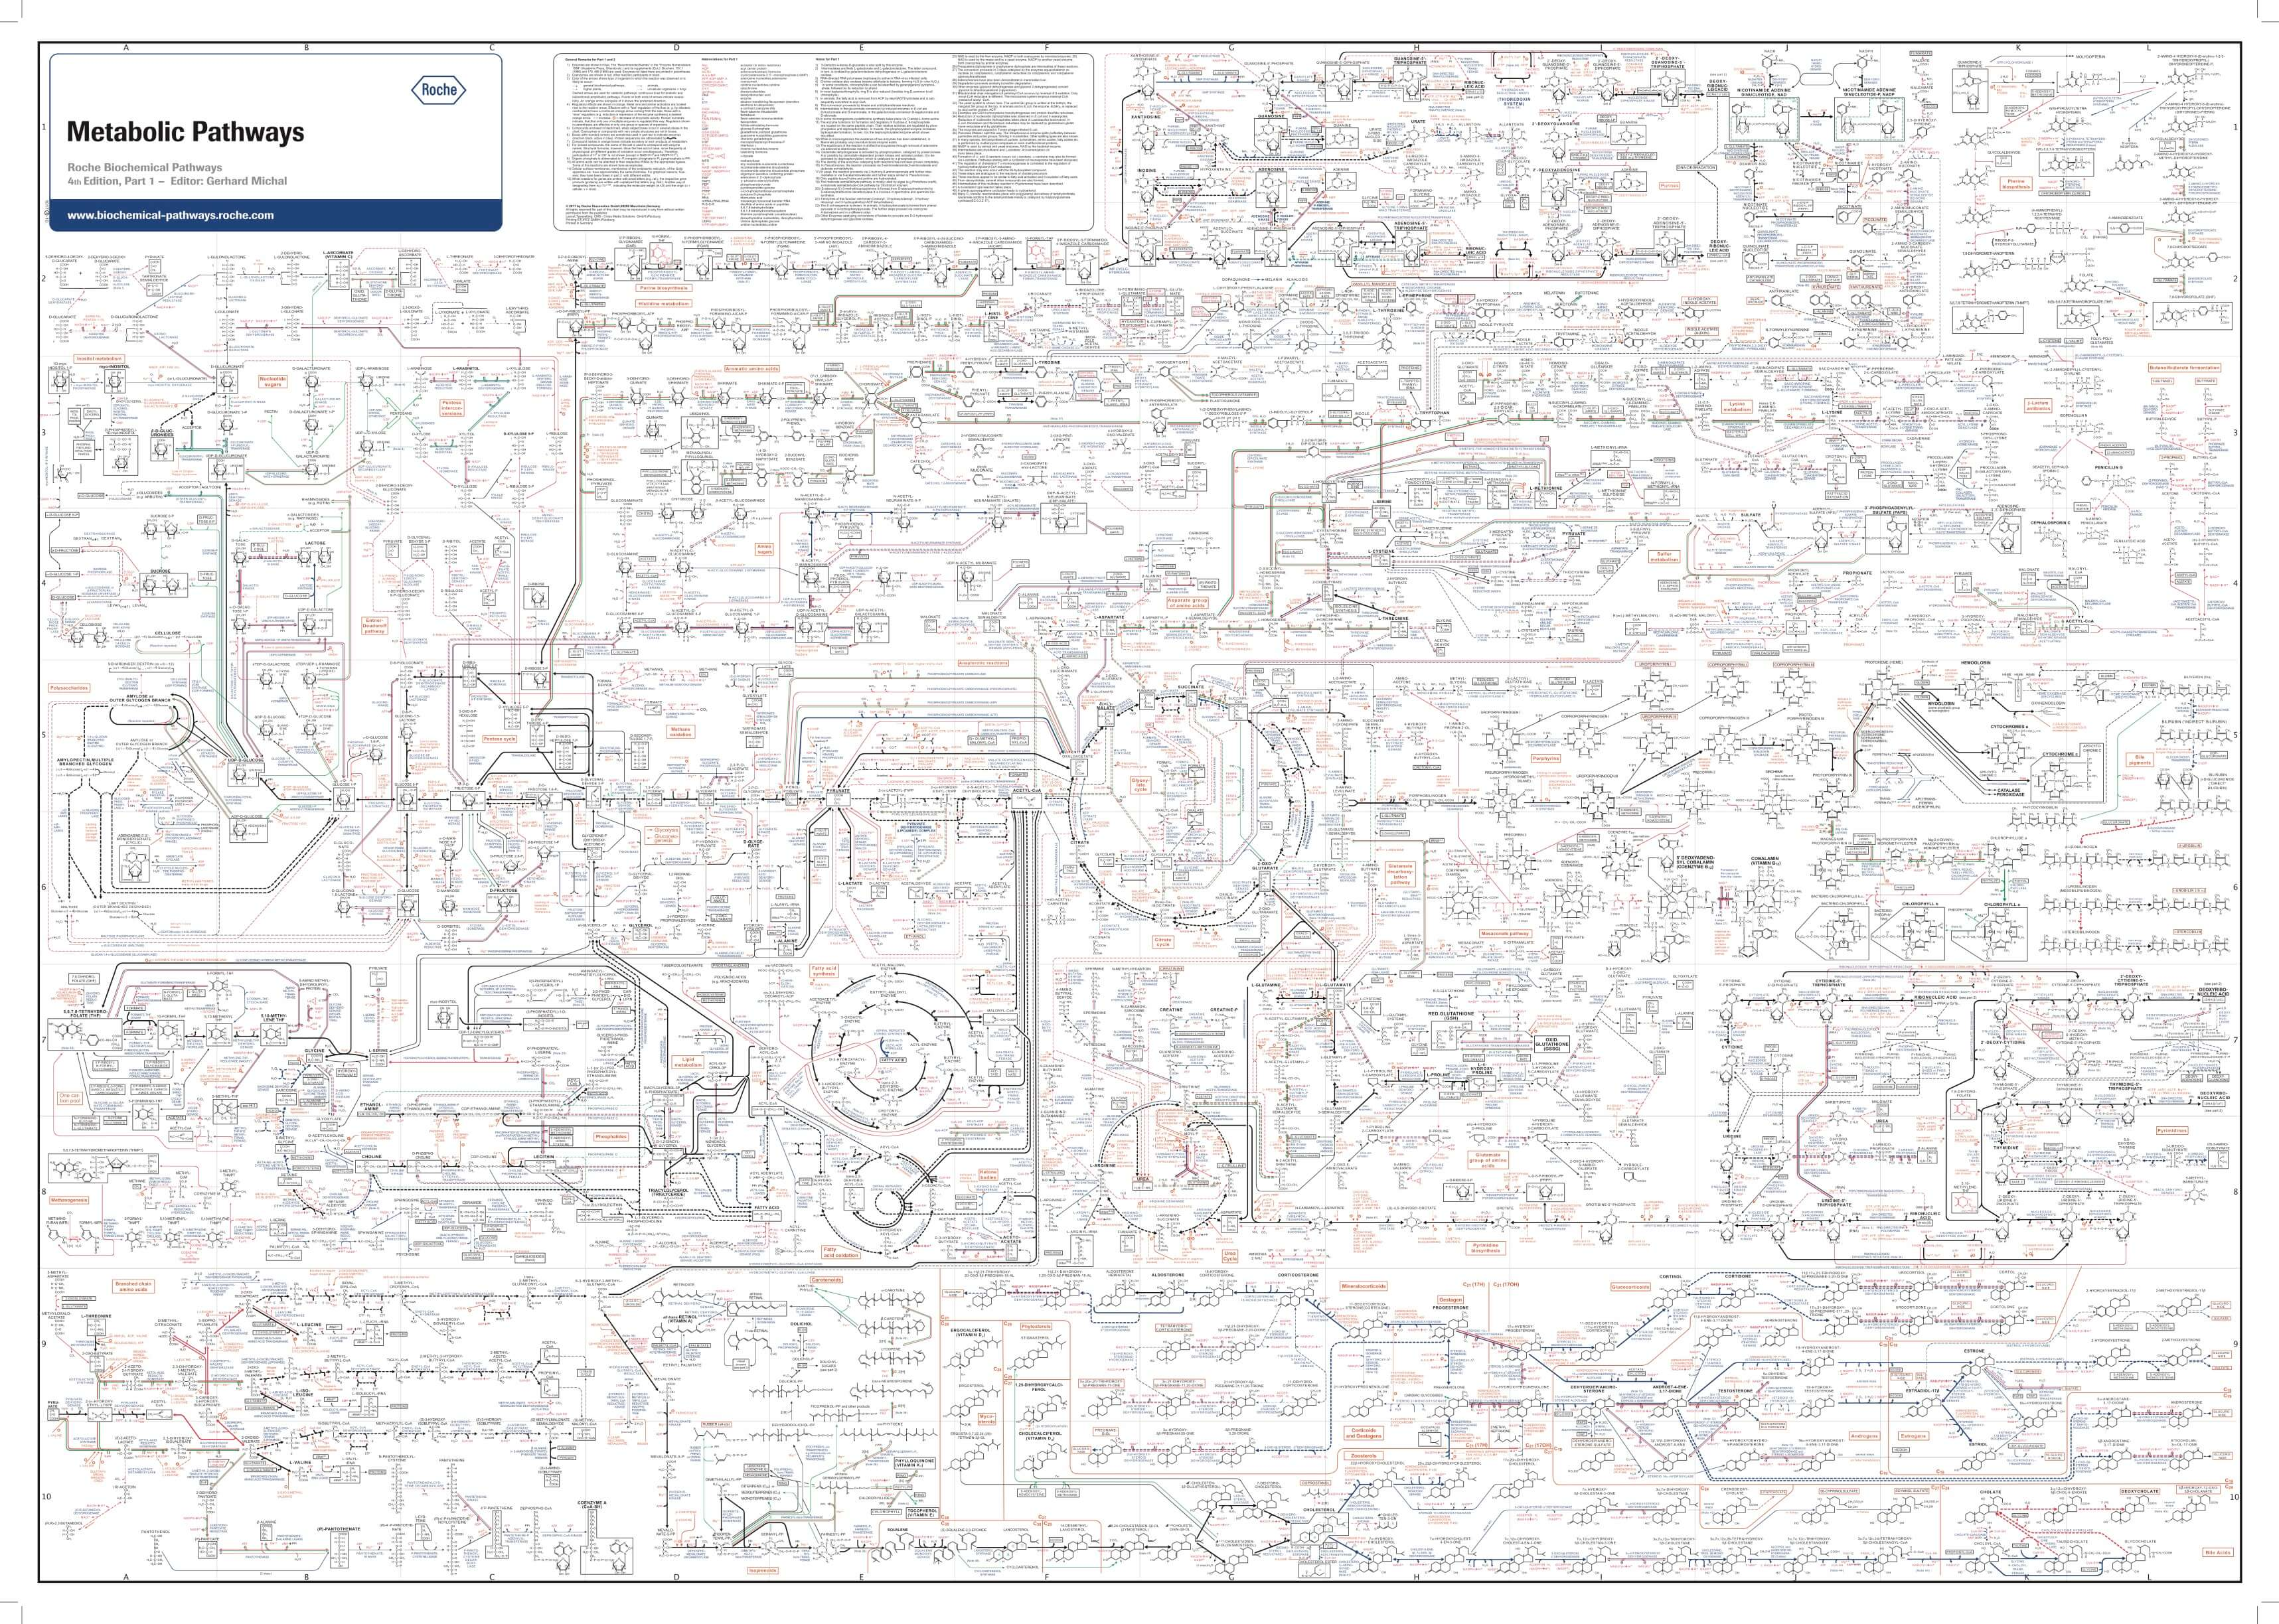
\includegraphics[width=1\linewidth]{./figs/roche_pathways} 

}

\caption{Network of the most important reactions in a living cell (Source: Dr. Gerhard Michal, Roche)}\label{fig:chemicalReactionsCell}
\end{figure}

\hypertarget{energy}{%
\subsubsection{Energy}\label{energy}}

``Life is Chemistry'' because it uses chemical reactions to store and use energy. See the ATP-ADP system in Section \ref{sectionEnergyCoin}

\hypertarget{catalysis}{%
\subsubsection{Catalysis}\label{catalysis}}

``Life is Chemistry'' because most chemical reactions are catalyzed, i.e.~initiated, promoted and made faster by proteins. The proteins facilitate the reaction without being used. The reactions would never take place if we would only mix the molecules at the concentrations that are typically occurring in a cell.

A catalyst is a chemical substance that helps a reaction to take place without being consumed. Proteins that are catalysts are also referred to as enzymes.

Enzymes are proteins that

\begin{itemize}
\tightlist
\item
  initiate the reaction
\item
  speed up the reaction and
\item
  make sure that the outcome is always the same.
\end{itemize}

Loosely speaking they are

\begin{itemize}
\tightlist
\item
  ``fishing'' certain molecules from the complex mixture in a cell,
\item
  which consists of thousands of chemical compounds generally at low concentrations,
\item
  through binding sites they can facilitate that these molecules (substrates) are getting close so that they can react and form a new compound.
\end{itemize}

These binding sites emerged from to the unique 3D structure of the protein, see Figure \ref{fig:enzyme}.

In most cases enzymes work together in pathways, which consist of multiple chemical reactions for which (part of the) molecules produced in the previous reaction are used by another enzyme to facilitate the next reaction.

A well known example of this is the Krebs cycle that is the main source of energy for a cell through metabolizing carbohydrates, lipids and/or proteins. It is a cyclic pathway of multiple chemical reactions each catalyzed by another enzyme (see Figure \ref{fig:krebsCycle} or the you tube movie \url{https://www.youtube.com/embed/yk14dOOvwMk}).

The Krebs cycle is also used to generate building blocks for constructing certain nucleotides and amino acids.

\begin{figure}

{\centering 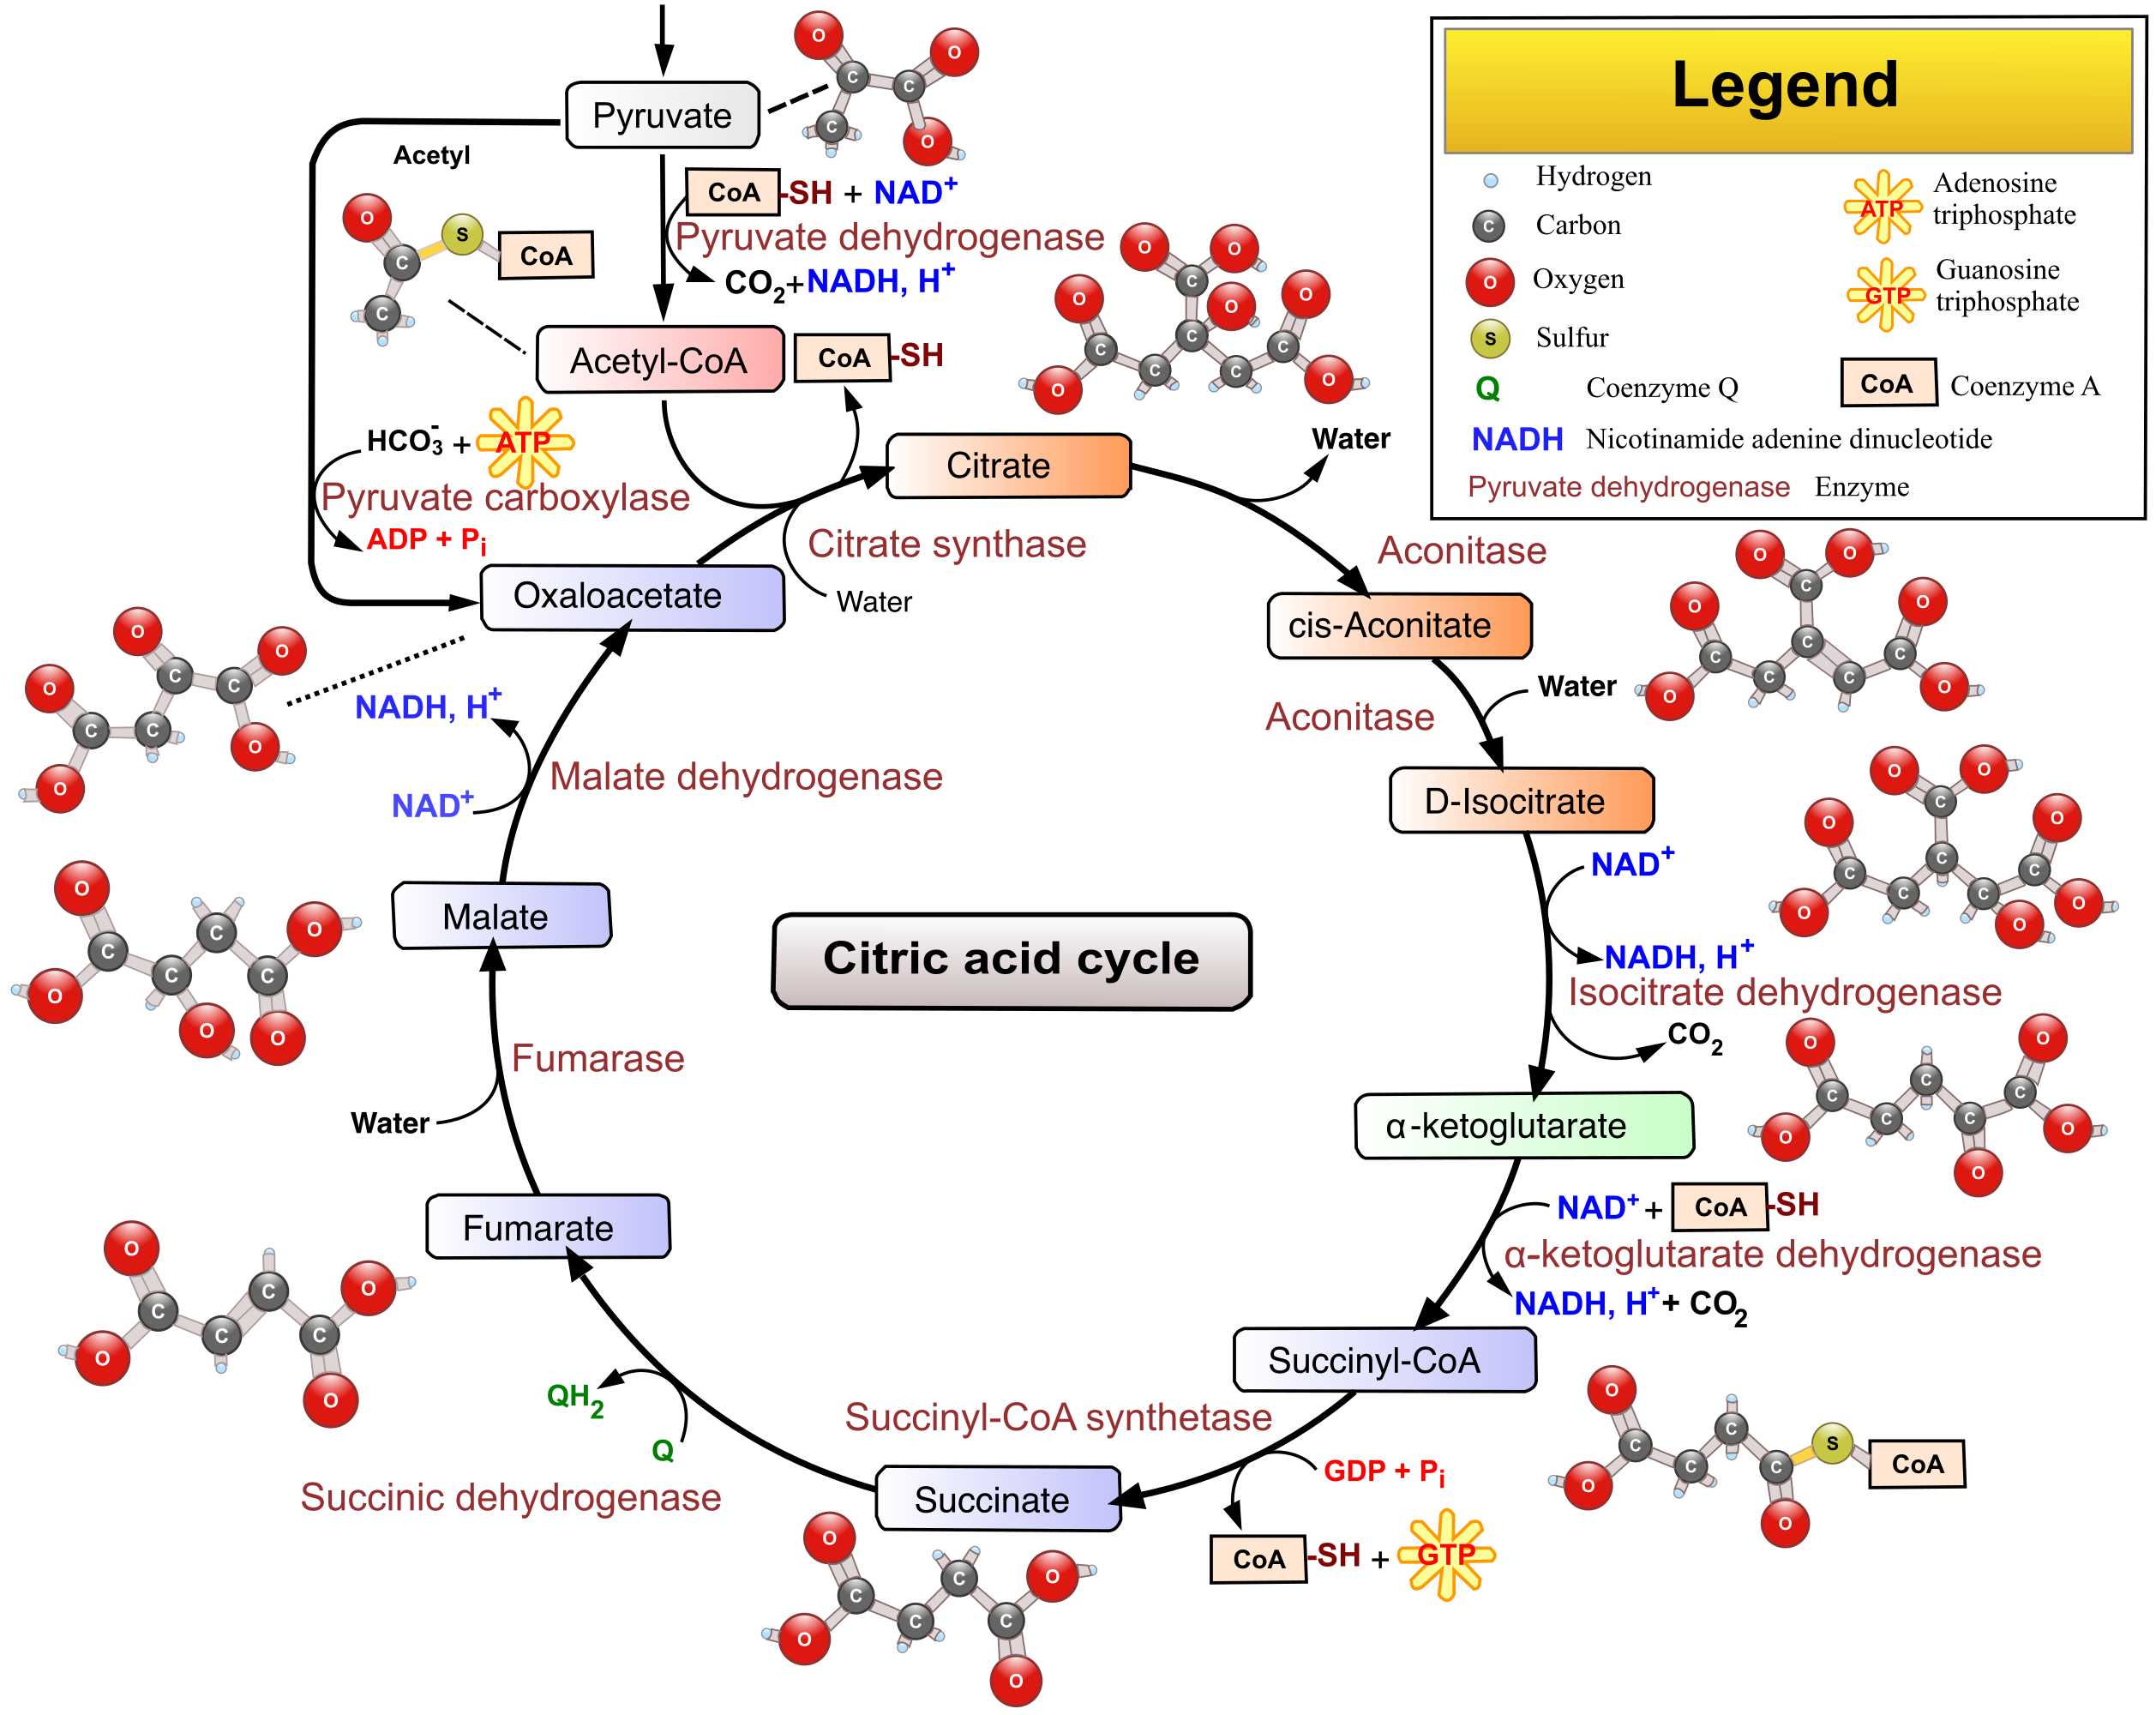
\includegraphics[width=0.7\linewidth]{./figs/Citric_acid_cycle_with_aconitate_2} 

}

\caption{Krebs cycle, a cyclic pathway connecting multiple reactions that provide the main source of energy for our cells by metabolising carbohydrates, proteins and lipids. Each reaction is catalised by an enzyme  (Source: Narayanese, Wikipedia)}\label{fig:krebsCycle}
\end{figure}

We can end this section with a quote of \citet{deDuve2002}: ``Any living organism is a reflection of its enzyme arsenal''.

\newpage

\hypertarget{self-organisation}{%
\subsubsection{Self-Organisation}\label{self-organisation}}

Life is also characterized by its ability for self-organisation. Some proteins are also important to give structure to a cell and they can spontaneously form structure.
An intriguing illustration of self-organisation is provided by \citet{Cheng2019} who
homogenized Xenopus laevis egg cytoplasmic extracts (liquid with structures form the cell) and showed that the homogeneous extract spontaneously reorganized itself in cell like structures in a matter of minutes (see Figure \ref{fig:selforganisation} and you tube movie \url{https://www.youtube.com/embed/prq1Occu22s}).



\begin{figure}

{\centering 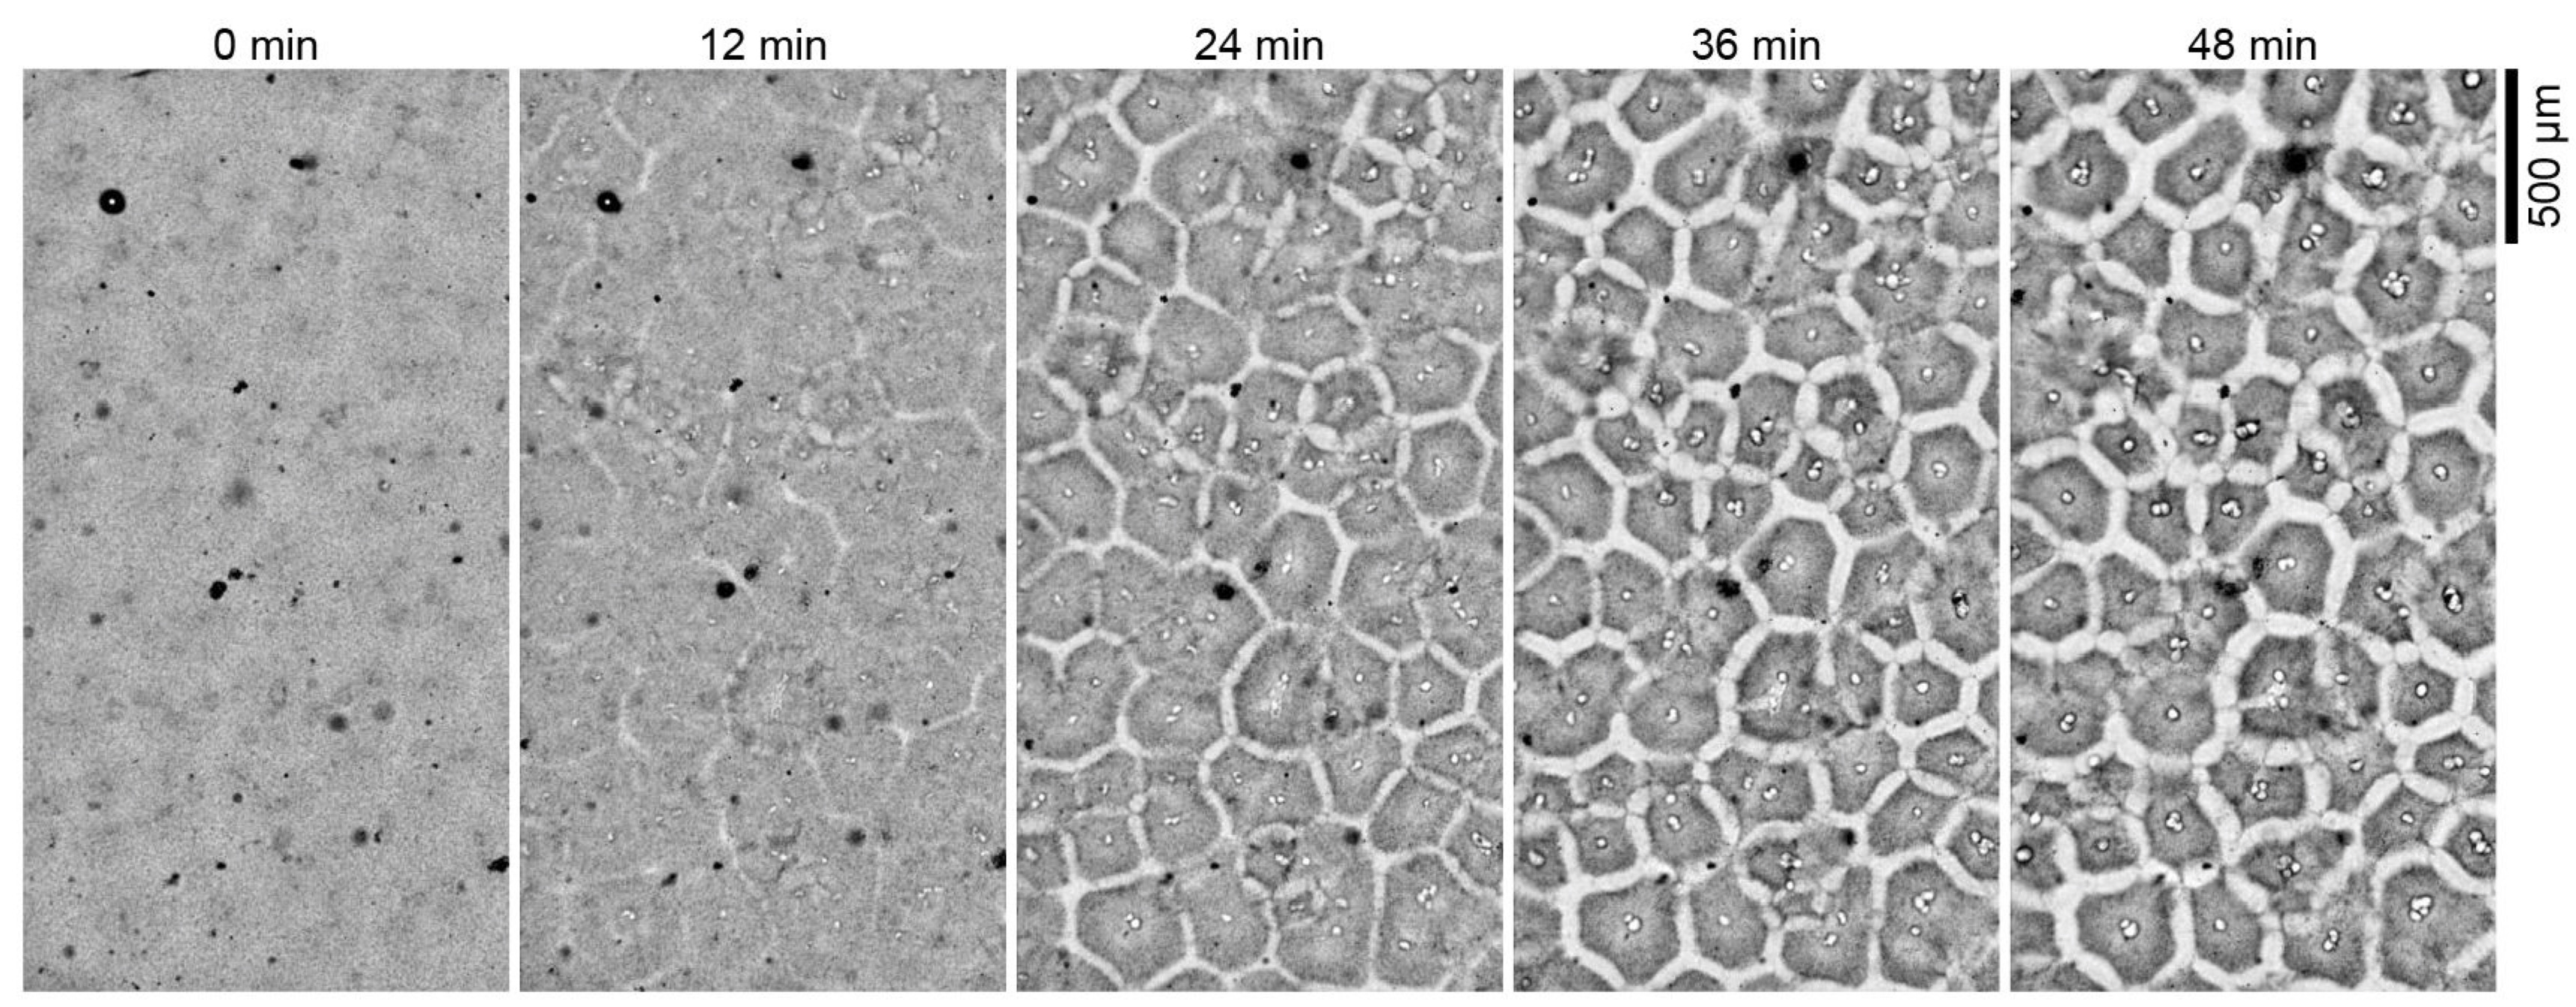
\includegraphics[width=1\linewidth]{./figs/selforganisation} 

}

\caption{Homogenized Xenopus laevis egg cytoplasmic extracts spontaneously organized into cell-like compartments \citep{Cheng2019}}\label{fig:selforganisation}
\end{figure}

\citet{Cheng2019} found that ATP, the energy source of a cell; microtubuli, a kind of filamentous proteins; and dynein, a kind of motor protein, were required and driving this process of self-organisation.

\begin{figure}

{\centering 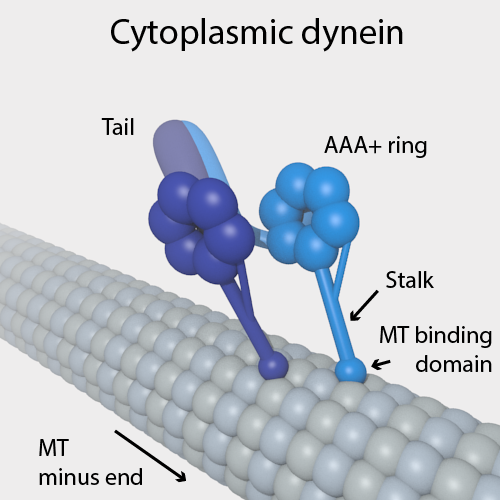
\includegraphics[width=0.3\linewidth]{./figs/DyneinHeavyChainOnMT} 

}

\caption{Microtubulus (long filamentous protein) with Dynein "motor" protein attached (Source:  Wikipedia)}\label{fig:dynein}
\end{figure}

Note, that proteins thus play a central role in life. They are key for catalysis and giving structure. Hence, a cell thus not only inherits genetic information, but, also its spatial organisation from a mother cell!

\newpage

\hypertarget{lifeInformation}{%
\subsection{Life is Information}\label{lifeInformation}}

DNA and RNA are hetero-polymers. They are build from 4 different nucleotides so the genetic information is stored in an alphabet of 4 letters. This is
adenine (A), cytosine (C), guanine (G) and thymine (T) for DNA and in RNA thymine (T) is replaced by uracil (U).
It makes no physical or chemical difference what the identity of the next nucleotide in the chain is. So they can seen as a coding system to store and pass genetic information from one generation to the next. Life is therefore also information and not only chemistry.

The ``central paradigm'' of molecular biology states that the sequence of nucleotides in DNA are first \emph{transcribed} into RNA and then \emph{translated} into proteins, see Figure \ref{fig:centralParadigm}.

Note, that some RNA molecules are also end products. Indeed RNA can also have a catalytic function, i.e.~initiate and promote chemical reactions without being consumed themselves.

A \emph{gene} is the unit of genetic material, a DNA sequence that is encoding for the synthesis of a gene product, either a protein or a functional RNA. The latter is also referred to as a non-coding RNA (ncRNA).

\begin{figure}

{\centering 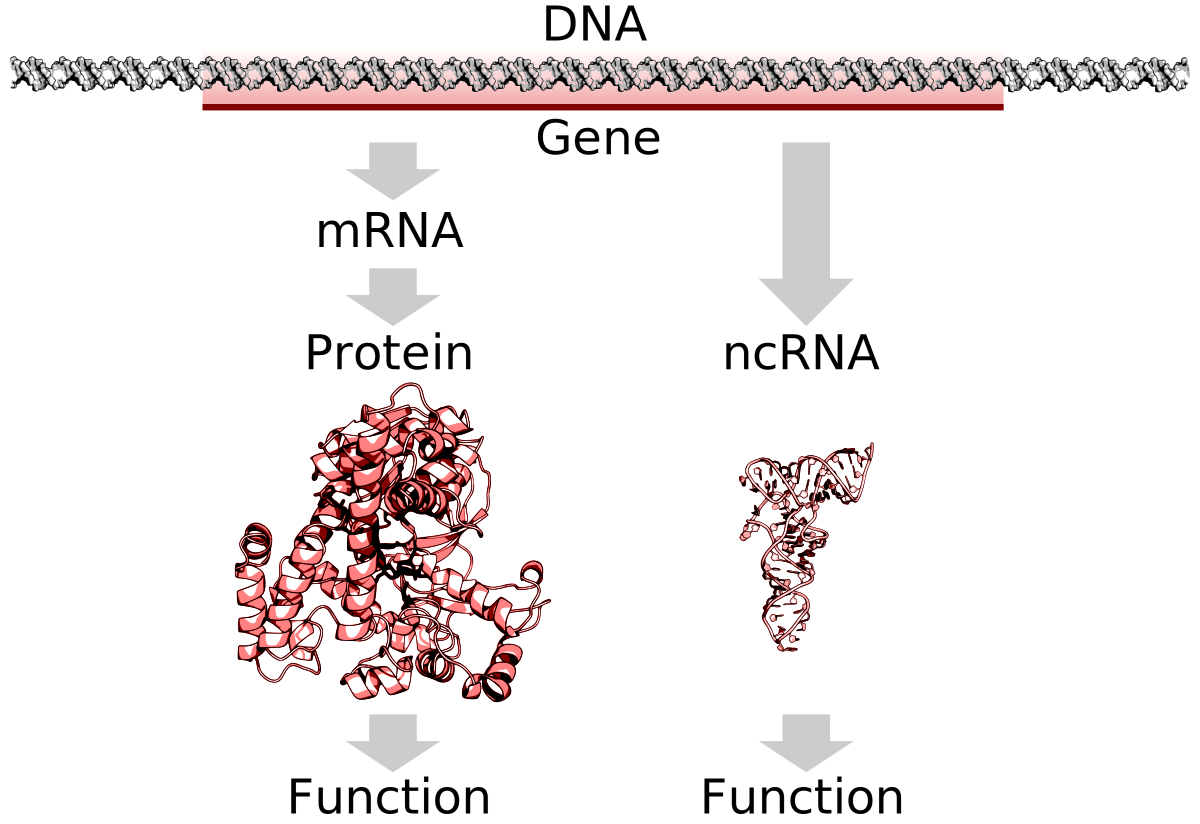
\includegraphics[width=0.5\linewidth]{./figs/gene} 

}

\caption{Central paradigm of biology: a gene, a specific region in the DNA, is first transcribed into RNA and then into proteins. Note, that for RNA-genes the RNA molecule is the end product itself, which is referred to as non-coding RNA (ncRNA) (Source: Thomas Shafee, Wikipedia)}\label{fig:centralParadigm}
\end{figure}

Figure \ref{fig:transcriptionTranslation} shows the process of transcription of a gene from DNA to RNA and the translation of RNA to proteins.

\begin{enumerate}
\def\labelenumi{\arabic{enumi}.}
\item
  The transcription of DNA to RNA is initiated by opening the
  DNA double strand. Then a complementary RNA strand is synthesized by exploiting that A hybridizes to U (or T) and G to C through hydrogen bounds.
\item
  Once that the complementary RNA strand is made, it is further processed in the nucleus into messenger RNA (mRNA). The mRNA travels from the cell nucleus to the cell cytosol (cell liquid) where it is translated into proteins, and, where the majority of the reactions take place.
\item
  There mRNA is translated into proteins by ribosomes.
  In the ribosomes the mRNA is bound to transfer RNA (tRNA). tRNA can bind to the mRNA molecule if it has 3 consecutive nucleotides that are complementary to the triplet of the 3 consecutive nucleotides on the mRNA template that is lying in the ribosome.
\item
  The transfer RNA transports one specific amino-acid that is then incorporated in the protein that is being formed, which is the growing amino acid chain in Figure \ref{fig:transcriptionTranslation}. The sequence of 3 consecutive nucleotides of DNA of a gene is therefore also called a \emph{codon} because it encodes for a specific amino acid.
\item
  Upon incorporation, the ribosome shifts to the next triplet of the mRNA and the next transfer RNA is bound to it, and so on until a stop codon is reached and the protein is finished.
\end{enumerate}



\begin{figure}

{\centering 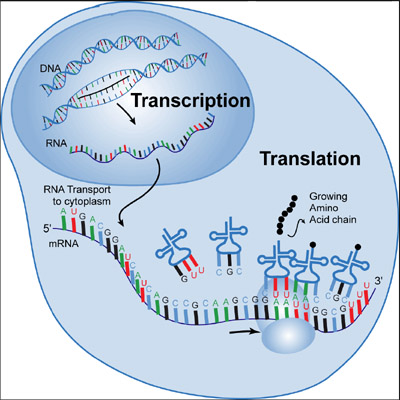
\includegraphics[width=0.5\linewidth]{./figs/transcription_2} 

}

\caption{In the cell nucleus the DNA strand opens up and is transcribed into an RNA molecule. Upon processing, the messenger RNA (mRNA) travels from the nucleus to the cytosol where it is translated into proteins. The mRNA is the template that fits into a ribosome that has the function to bind transfer RNA molecules to the mRNA template. It does that by hybridizing to a tRNA, which has a triplet of three nucleotides that are complementary to those of the mRNA template. The tRNAs have a amino acid on their tail, which is incorporated into a long chain of amino acids, the protein that is produced. If the amino acid is incorporated, the ribosome moves to the next triplet and the process happens all over with a new tRNA (Source: \href{http://www.tokresource.org/tok_classes/biobiobio/biomenu/transcription_translation/}{tokresources.org})}\label{fig:transcriptionTranslation}
\end{figure}

There are in total 64=4\(^3\) codons encoding for each of the 20 amino acids, and, for a start and a stop codon to initiate and stop the protein translation, respectively. Hence, there is a redundancy in the code, see \ref{fig:codonTable}.

\begin{figure}

{\centering 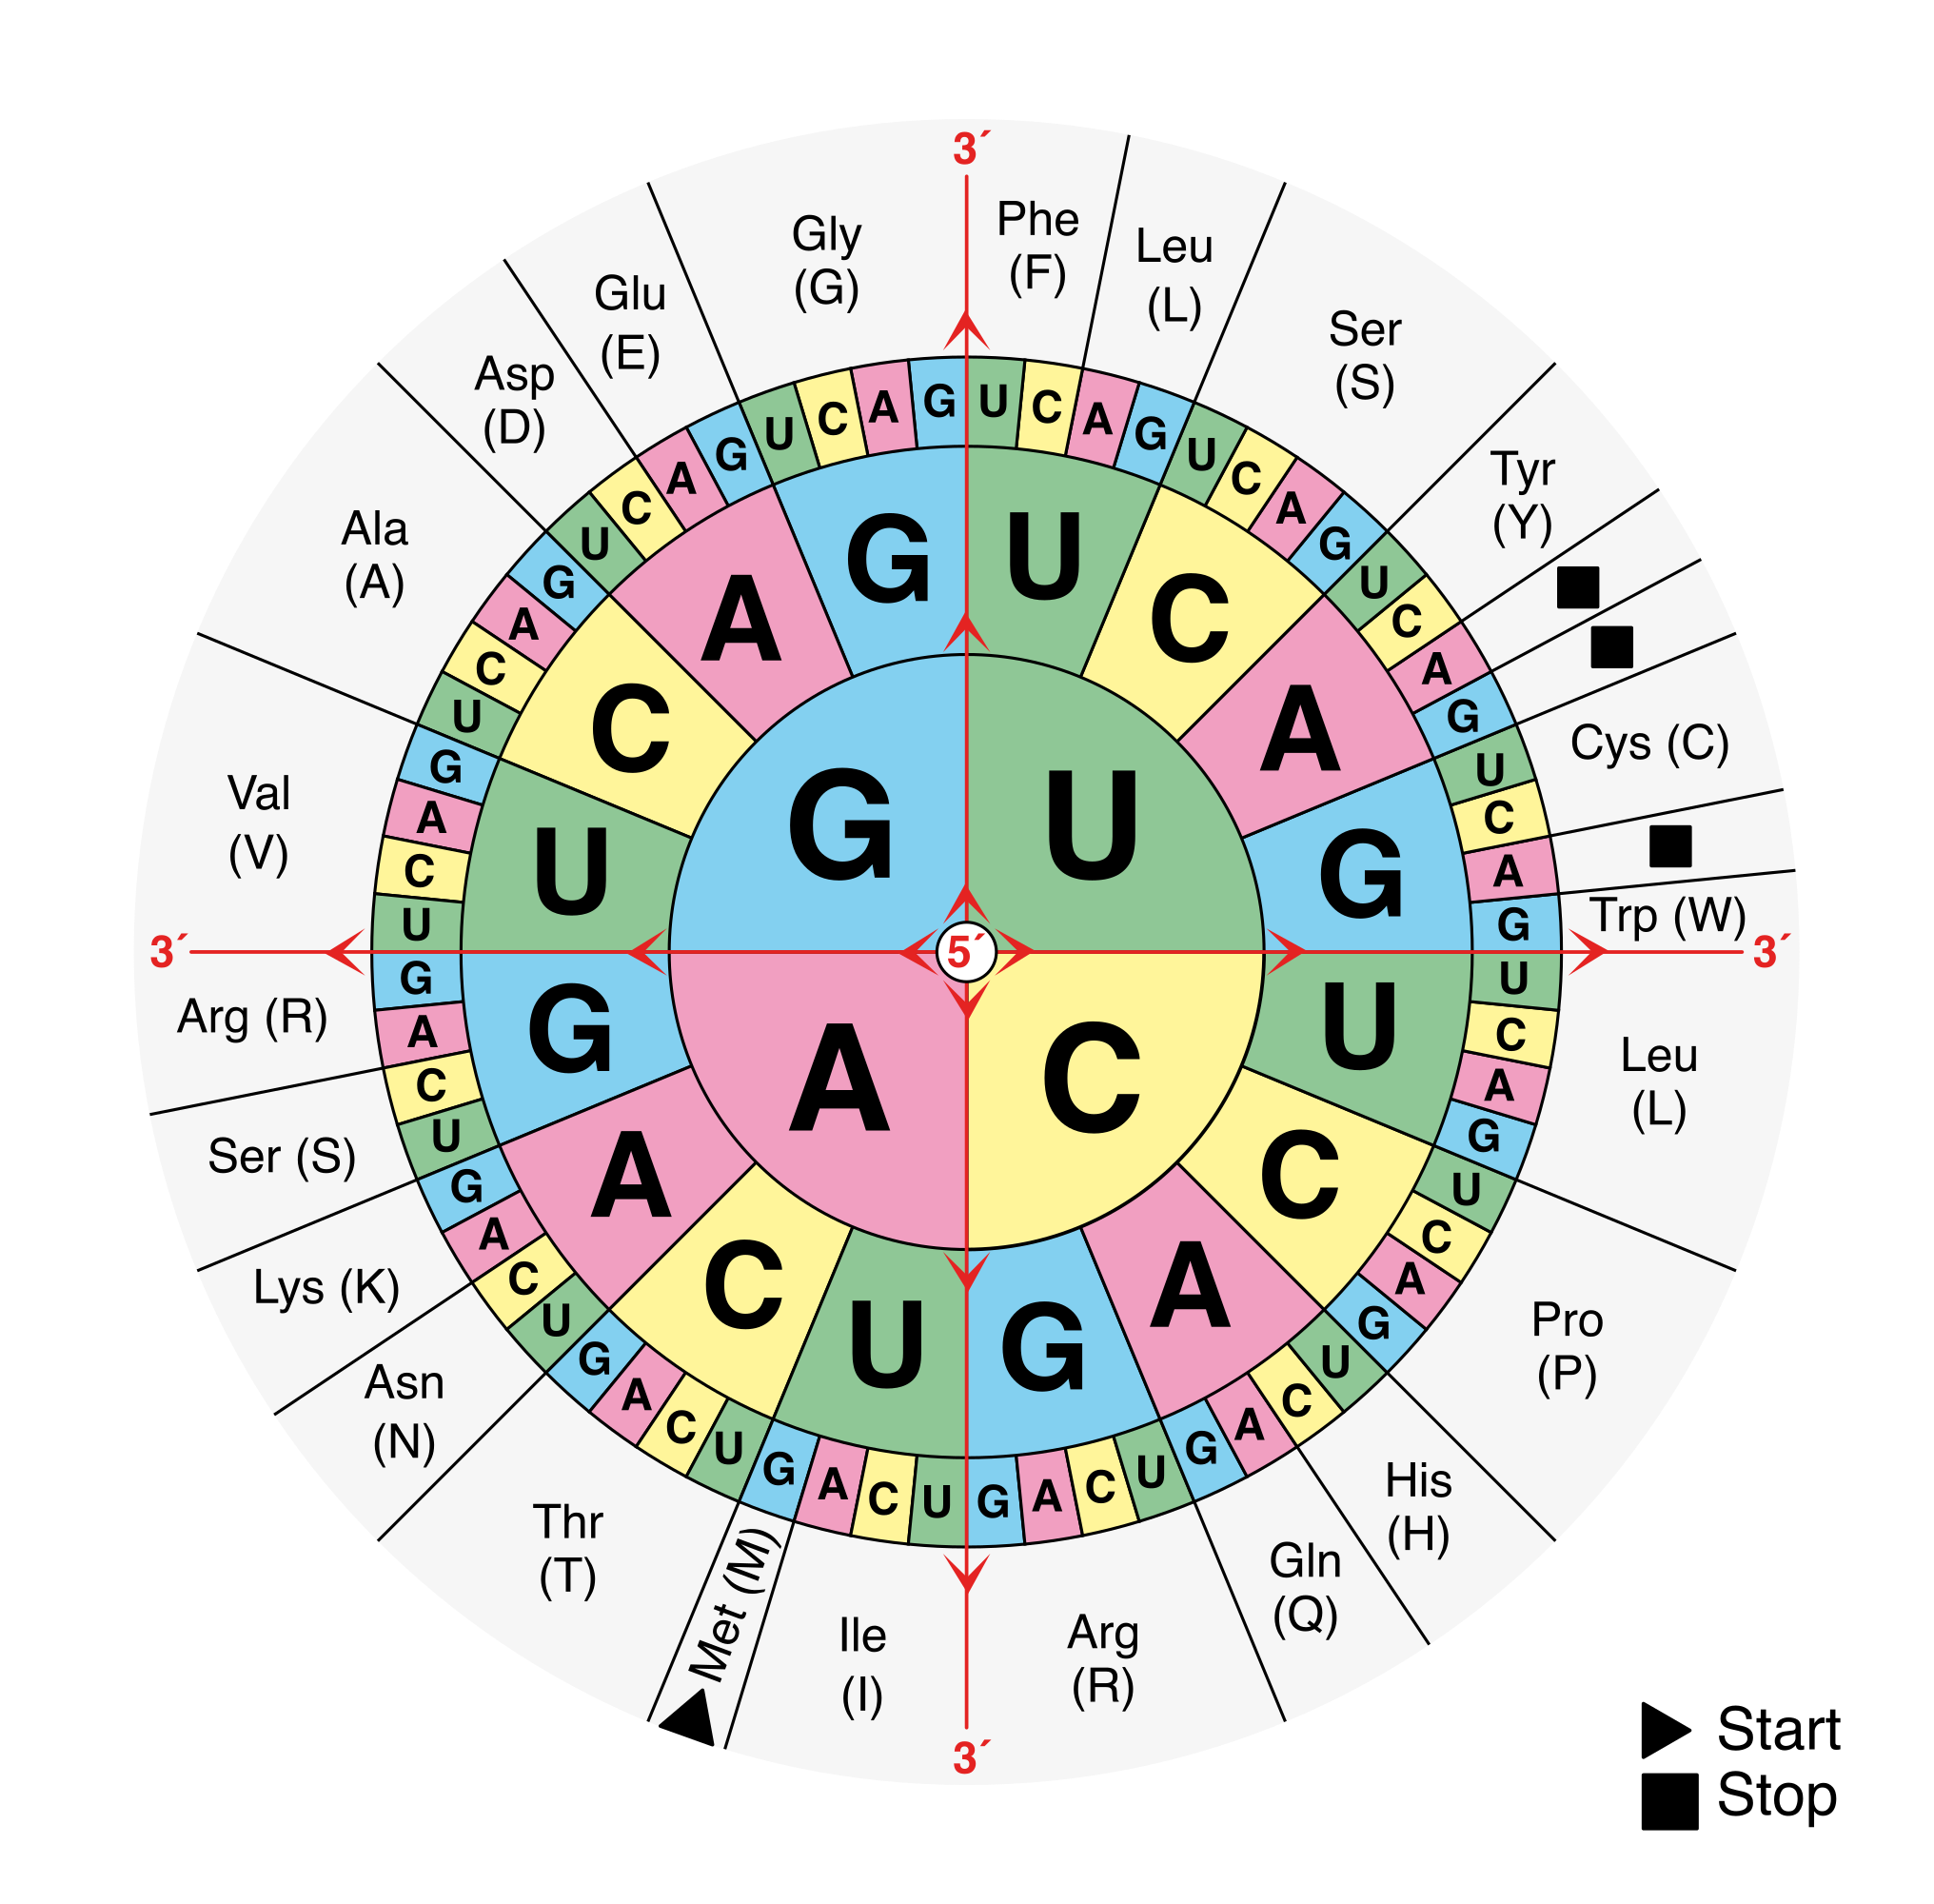
\includegraphics[width=0.5\linewidth]{./figs/Aminoacids_table} 

}

\caption{Codon table connecting triplets of nucleotids to amino acids (Source: Wikipedia)}\label{fig:codonTable}
\end{figure}

We can learn an important message from the codon table:

\begin{itemize}
\item
  There is no chemical necessity that explicitly connects the three nucleotides ``CGG'' to the amino acid arginine rather than to glutamine.
\item
  Nucleotides themselves do not seem to a have chemical connection to the amino acids they encode
\item
  Therefore we call it a code or information rather than just ``genetic chemistry''
\end{itemize}

The code apparently evolved so that many mutations give rise to

\begin{itemize}
\tightlist
\item
  synonymous codons (same amino acid) or
\item
  to incorporate amino acids that are similar
\end{itemize}

so that protein function is conserved.

DNA is thus the carrier of genetic information. However, RNA plays a more central role:

\begin{itemize}
\tightlist
\item
  Messenger RNA brings the genetic information from the cell nucleus to the cell cytosol where they are translated into proteins and where most of the chemical reactions take place.
\item
  Ribozymes, i.e.~catalytic RNA molecules, initiate and speed up particular reactions
\item
  Transfer RNA plays an crucial role in the translation of proteins
\item
  An RNA primer, i.e.~a small RNA molecule, is essential to copy DNA
\item
  RNA also acts as carrier of genetic information, e.g.~corona virus.
\end{itemize}

\newpage

\hypertarget{maturana-and-varela-a-systems-view-of-life}{%
\section{Maturana and Varela: a Systems View of Life}\label{maturana-and-varela-a-systems-view-of-life}}

In the theory of the module on Biological Aspects of Biodanza Rolando Toro also introduced the term \emph{autopoiesis}.

\citet{capraLuisi2014} write in their book ``The system view of life'', that the ``term was coined by Varela and Maturana in the 1970s. \emph{Auto}, of course, means \emph{self} and refers to the autonomy of self-organizing systems; and \emph{poiesis} (which shares the same Greek root as the word poetry) means \emph{making}. So, \emph{autopoiesis} means self-making''.

They continue stating that ``the main characteristic of life is self-maintenance due to internal networking of a chemical system that continuously reproduces itself within the boundary of its own making''.

Indeed, a living cell is the smallest autopoietic unit.
The cell consists of a complex internal network of chemical reactions and this within the boundary of its outer membrane.
It can organize itself, maintain itself, can make copies of itself and this with the enzymatic machinery that is present in the cell itself.

Networks of cells are then combined in larger autopoietic units, e.g.~

\begin{itemize}
\tightlist
\item
  our gut microbiome that consists of a network of billions of unicellular bacteria from which unique metabolic functions emerge that are essential for digesting our food, or,
\item
  our tissues, networks of our own cells from which novel functions emerge.
\end{itemize}

An organism or a biological system can therefore not be broken down or reduced to its parts to provide a complete understanding of it. A complete understanding is only possible when it is viewed as a whole.
Indeed, new functions emerge at a higher level from the network that has been formed between its lower-level parts. Varela refers to these properties with the term \emph{emergent properties}.

Emergent properties can be found at each level. At the chemical level, where the protein hemoglobin for instance has the unique property that it can transport oxygen. This property emerges from its unique 3D structure of four sub-units each with an iron atom at its center (see Figure \ref{fig:hemoglobin}). We could never have derived its biological function at the protein-level by breaking it down to its constituting amino acids and only studying the individual properties of each of these amino acids.

\begin{figure}

{\centering 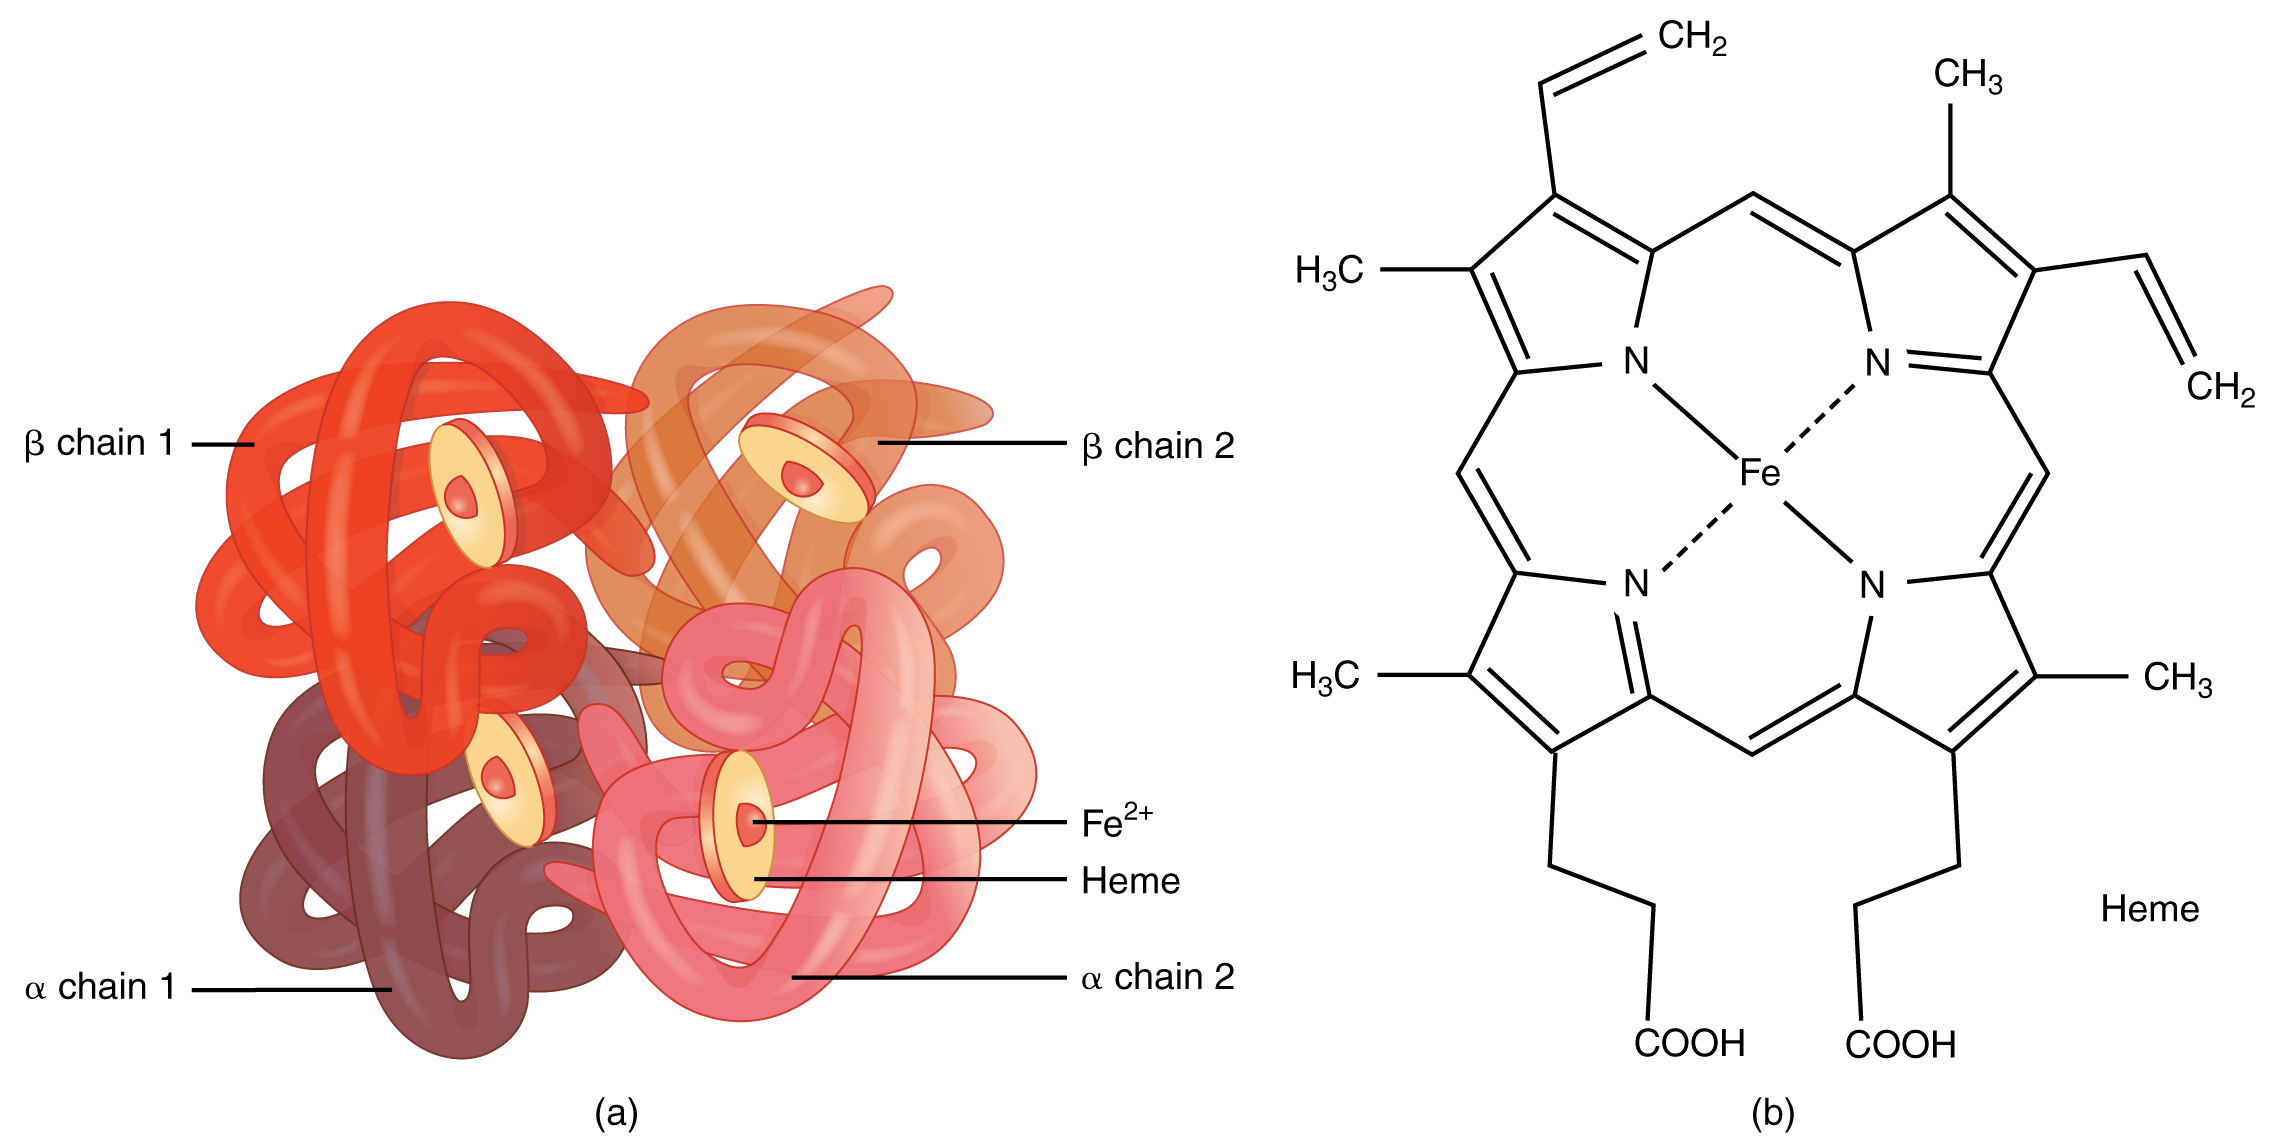
\includegraphics[width=1\linewidth]{./figs/hemoglobin} 

}

\caption{Structure of hemoglobin that consists of 4 subunits, each having a heme group with an iron molecule that can bind oxygen. This function emerges from its unique 3D structure (Source: Wikipedia)}\label{fig:hemoglobin}
\end{figure}

So hemoglobins' property to transport oxygen naturally emerges at the protein level upon combining many simple amino acid molecules in the appropriate sequence. Indeed, this specific long chain of amino acid spontaneously folds into a unique 3D structure that gives the hemoglobin protein its unique function.

\citet{capraLuisi2014} convincingly argue that the same holds at any level and for life itself. Indeed the autopoietic property of a cell originates by properly combining all its molecules in the large networks of chemical reactions from which its structure and organisation, self maintenance, and self replication emerge.

We cannot localize life. Life is simply a global property that emerges from the collective interactions of all kind of molecules in a cell, of the collection of cells in a tissue, of the collection of tissues in a organ system, of the collection of organ systems for an organism, of the collection of organisms in a population etc.
At each level we have a network of lower level components from which new properties naturally emerge.

So life itself is an emergent property, it is not present in the parts it originates from, and only emerges when its parts are assembled together correctly. If we perform the horrific experiment of putting a frog in a blender, life, its ultimate emerging property disappears irrespective from the fact that matter remains to a large extent the same. Studying the frog by solely studying its blended components will not let us understand how a frog is functioning.

For Maturana and Varela cognition is also inseparable from autopoiesis \citep{capraLuisi2014}. Each living organism is an open system that interacts with its environment through its sensory arsenal. It senses its environment, it feeds on its environment, releases products in it, it changes its environment, and, actualizes itself to its environment. The fact that an organism is changing its environment is often overlooked. However, life has dramatically transformed Earth. Indeed, think of photosynthesis for instance that radically changed Earth by the release of the highly reactive molecule oxygen.

So an organism at any time in its development is a record of its previous interactions with its environment and that determines its future interactions.
Hence, cognition is a natural product of its evolution.

Varela sees life as a gestalt of three domains \citep{capraLuisi2014}:

\begin{itemize}
\tightlist
\item
  Environment,
\item
  Cognition and
\item
  The autopoietic unit.
\end{itemize}

Life is the synergy of these three domains, which he refers to as the embodied mind.

The insights of Maturana and Varela have the compelling implication that we no longer need to duality of matter and soul when trying to understand life. Life naturally arises as an emerging property of the large networks of matter or molecules at the level of each individual cell, the basic autopoietic unit, and then new properties emerge at a higher level when combining autopoietic units into tissues, organs, organ systems, communities, etc.

As such, we can also view our cognitive awareness as an emerging property of the network of our neurons in our brain in response to the history of our interactions with our environment, and this without needing the concept of the soul as an explanation.

\hypertarget{links-to-vital-unconciousness}{%
\section{Links to Vital Unconciousness}\label{links-to-vital-unconciousness}}

``Life is One'', all species originated from the same population of ancestral cells, they use the same chemistry, and the same encoding system to store their genetic information.
The wealth of living species, all with their own sensory arsenal, have been shaped through evolution by interactions with their environment.
So we can feel that all living beings are intimately connected.

The cells of living organisms act on internal and external stimuli by producing biochemical molecules, proteins, hormones, neurotransmitters, which in term shape their response.
Our response on ecofactors in the environment is largely determined by our embodied mind. This embodied mind emerged from the different levels of autopoietic units of which our organism consists together with the history of the interactions with the environment that we had ourselves, that of our ancestors and that of the species from which we evolved.

This intimate connection to life that is one, through our embodied mind, is in my opinion what Rolando was referring to with the term \emph{vital unconsciousness}.

So it becomes clear that all beings are sharing a kind of common cognition and this from ecosystem, population, organism, tissue, down to the cellular level. The latter which Rolando also referred to as a kind of \emph{cellular psychism}: with a memory, and an ability for affinity, repulsion, solidarity and communication as well as recognition of similar autopoietic structures in other forms of life.

So this \emph{cellular psychism} or \emph{vital unconsciousness} encompasses the origin of our instincts, bodily sensations and deeper knowledge that we can experience immediately from our embodied mind, without interference of our cognitive mind. Vivencia is a path to deeply connect, ameliorate and heal the vital unconsciousness, and, this along the five lines of Biodanza.

\hypertarget{links-to-the-biocentric-principle}{%
\section{Links to the Biocentric Principle}\label{links-to-the-biocentric-principle}}

I introduced the Biocentric principle in Section \ref{sectionBiocentricPrinciple}. When formulating his principle, Rolando started from the axiom that ``life is the essential condition for the genesis of the universe''.

From my background as a scientist this axiom does not seem to be a requirement for the deep effects and properties that can be deduced from the Model of Biodanza. It seems somewhat connected to the question ``What came first: the chicken or the egg?'' For me, biocentrism ``an sich'' i.e., starting from the deep astonishment that life as we know it simply exists and put it at the hearth of our weltanschauung, is a sufficient condition for the entire system of Biodanza.

This comprehension also triggered me not to elaborate on the ``Principi di Vita Cosmica'' explicitly in Section \ref{sectionModelOfBiodanza} ``Model of Biodanza'' in the introduction. Nevertheless, I feel that the introduction is entirely line with Rolando's method that starts from the simple fact that Life exists, here and now, and that knowledge originates through the Vivencia of Life itself. The latter triggers us to think about our origin and our place in the universe, and, more importantly to simply experience and deeply know it from within, and this without the burden of a mental process standing in between.

Prigogine and Stengers' book ``Order Out of Chaos'' \citep{prigogineStengers1984}, Capri and Luigi's book ``The Systems View of Life'' \citep{capraLuisi2014}, and, Rolando's axiom of the biocentric principle, however, invited me to rethink my definition of ``Life''. Instead of the narrow interpretation of ``Life as something biological'', I am pervaded by a broader vision originating from the astonishment and power that lies in dissipative self-organizing structures that are so omnipresent in our universe, and, of Capri's and Luigi's view that the whole biosphere can be viewed as a large autopoietic unit.

From this broader vision, can't we discern movement, dance, vitality, or life in dissipative self-organizing physical phenomena like a tornado or a swirling solar wind? And would this not allow us to define the dissipative structure to which such a natural system far from equilibrium organizes itself, its attractor, simply as Rolando did by referring to it as ``Life'' itself? Is this what Rolando meant with his quote that ``the universe is a living hologram''? So, was my choice to omit the ``Principi di Vita Cosmica'' in the introduction not simply a matter of semantics?

Now that we developed a basic understanding of how Rolando Toro viewed life, we will elaborate in the remaining chapters of this monograph on where, how and why the biological aspects can be found in the Model of Biodanza.

\hypertarget{principles-of-cosmic-life-and-the-genesis-of-life}{%
\chapter{Principles of Cosmic Life and the Genesis of Life}\label{principles-of-cosmic-life-and-the-genesis-of-life}}

The biological aspects are the vertical axis of the Model of Biodanza.
At the bottom of the model, we first encounter the Principles of Cosmic Life and the Genesis of Life, which are indicate with the red box in Figure \ref{fig:modelCosmic}.

\begin{figure}

{\centering 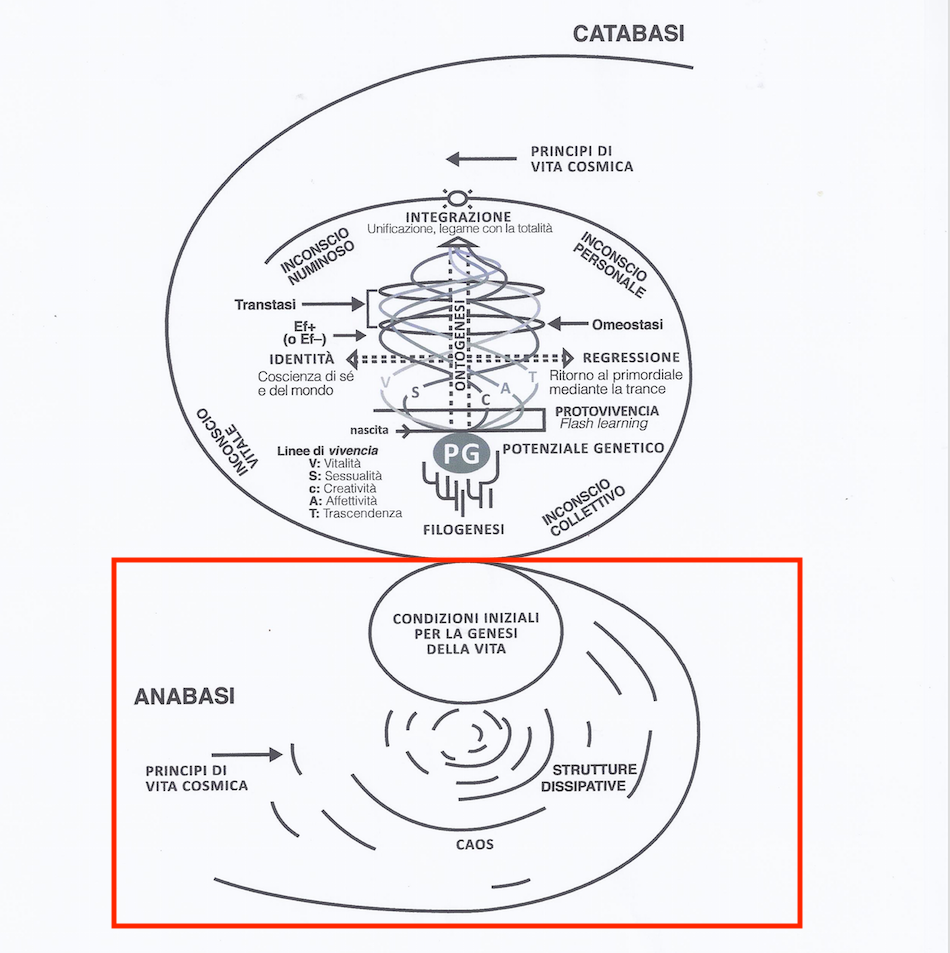
\includegraphics[width=0.5\linewidth]{./figs/biologischeAspectenBiodanzaDeelI} 

}

\caption{Model of Biodanza and Principles of Cosmic Life and the Genesis of Life}\label{fig:modelCosmic}
\end{figure}

We will start with the genesis of the universe and we conclude with the genesis of life.

\hypertarget{genesis-of-universe}{%
\section{Genesis of Universe}\label{genesis-of-universe}}

An overview of the evolution of our universe is given in Figure \ref{fig:evolutionUniverse}.

\begin{figure}

{\centering 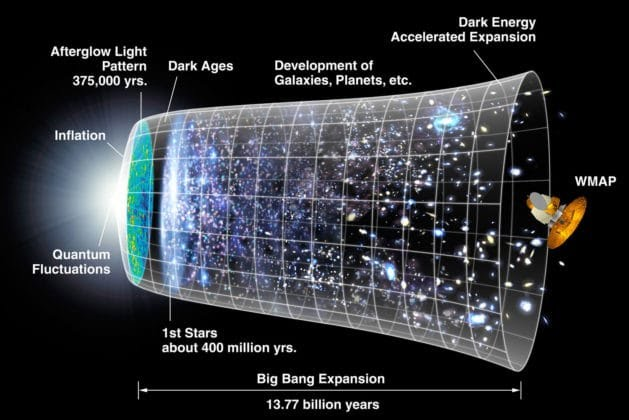
\includegraphics[width=1\linewidth]{./figs/originKosmos} 

}

\caption{Genesis and Evolution of our Universe (Source: NASA/WMAP Science Team, Wikipedia)}\label{fig:evolutionUniverse}
\end{figure}

The most common theory is that our cosmos started with the Big Bang.
A very energy-rich state.

By expanding the universe quickly cooled down enough for energy to be converted into mass, i.e.~the majority in hydrogen and a fraction in more heavy helium nuclei.

\hypertarget{genesis-of-stars}{%
\subsection{Genesis of Stars}\label{genesis-of-stars}}

Under the influence of the gravitational force, matter then started to cluster in nebula, gaseous clouds essentially consisting of hydrogen (H) and helium (He).

Due to concentration difference in these first nebula, these clouds further contracted and eventually imploded (See Figure \ref{fig:genesisStar}).

\begin{figure}

{\centering 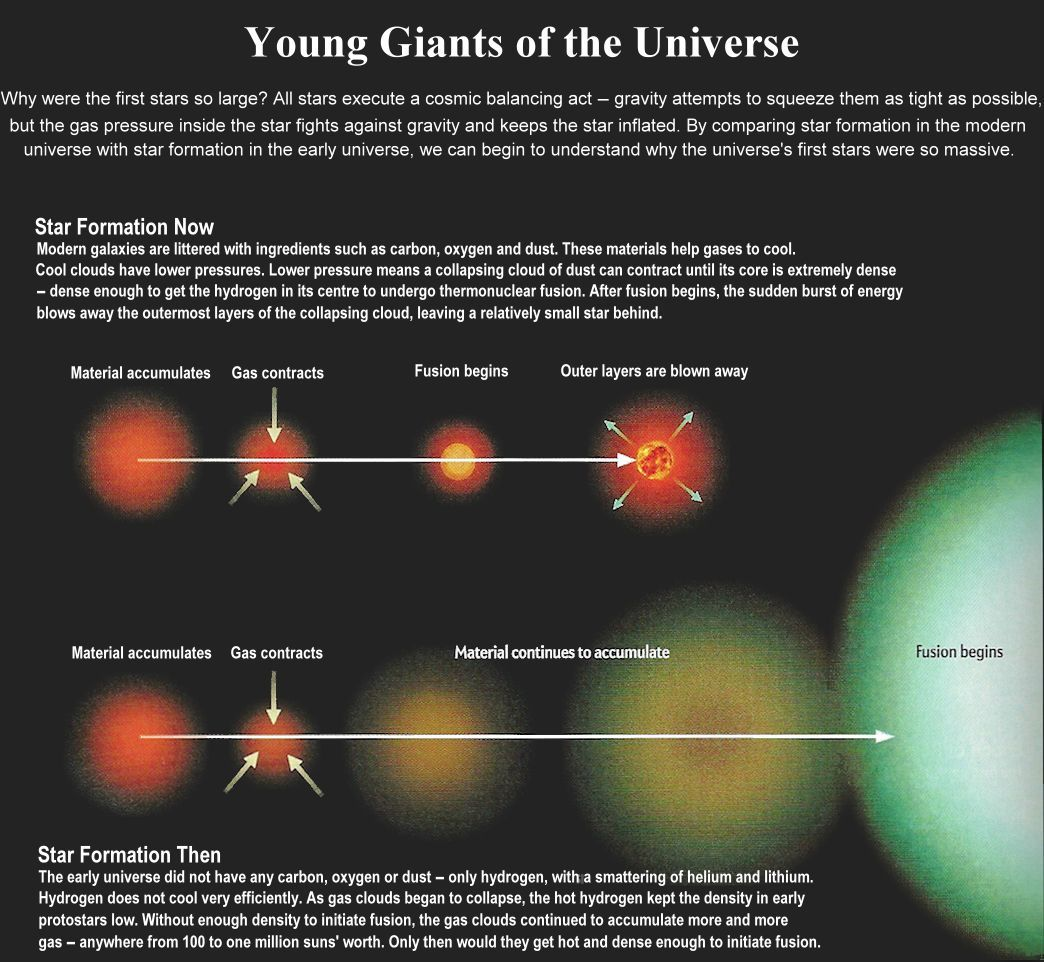
\includegraphics[width=1\linewidth]{./figs/I08-13-firststars6} 

}

\caption{Genesis of the first stars (Source: universe-review.ca)}\label{fig:genesisStar}
\end{figure}

Extreme heating in the nebula that imploded by gravity gave rise to a condition in which all matter was in the form of a super hot plasma.
In such a plasma nuclear fusion spontaneously takes place. In this process light atoms are combined into more heavy atoms and much energy is released.

First all hydrogen atoms are converted into helium (see Figure \ref{fig:nuclearFusion}).

\begin{figure}

{\centering 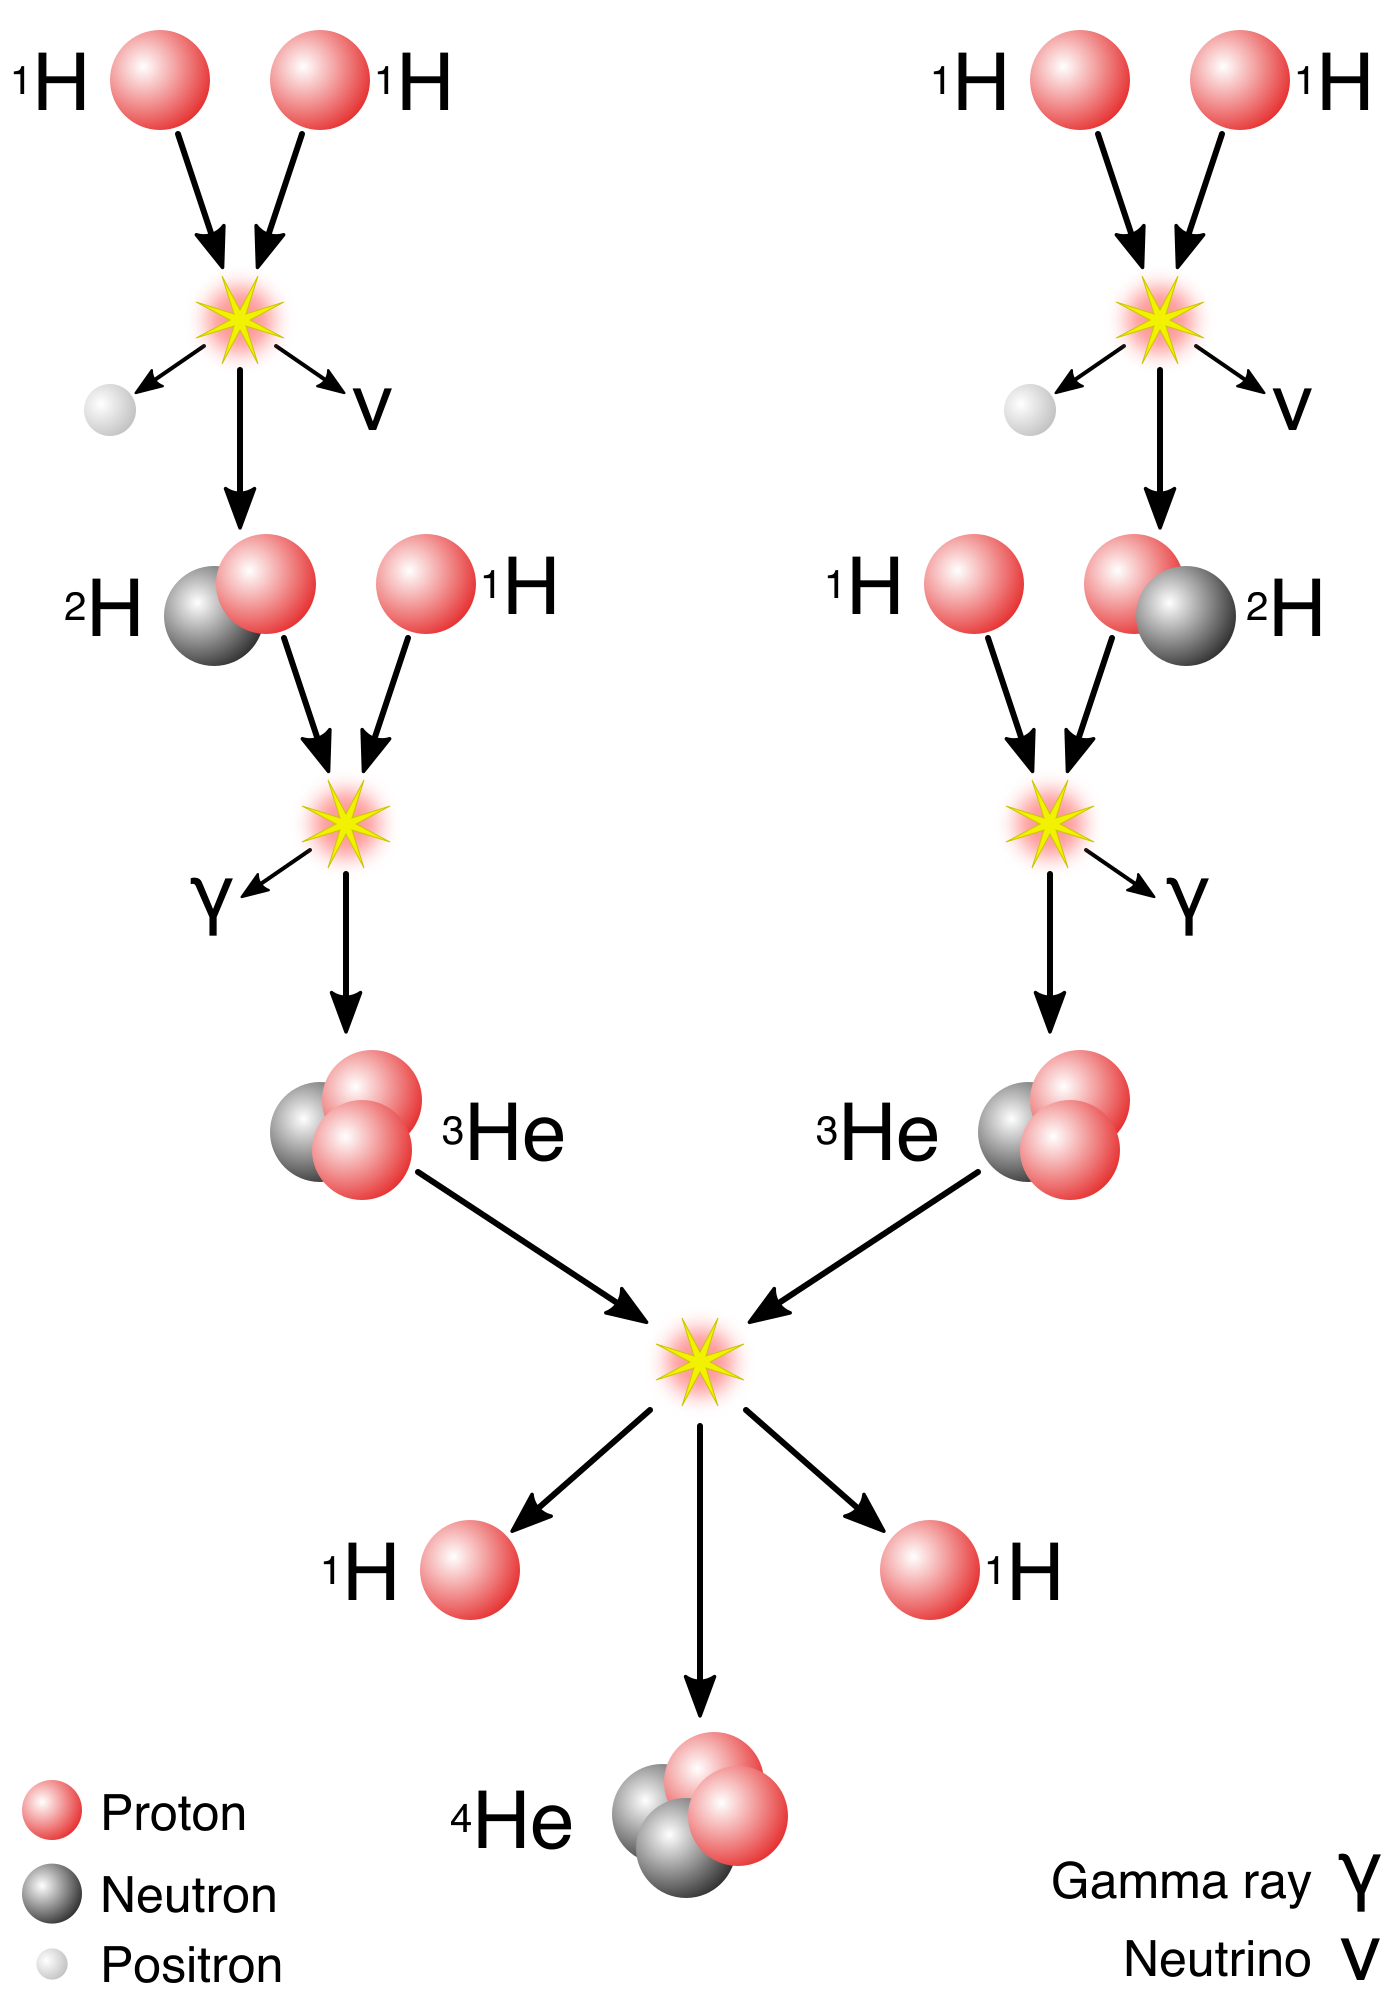
\includegraphics[width=0.5\linewidth]{./figs/fusion} 

}

\caption{Nuclear Fusion of hydrogen to the more heavy helium (Source: Sarang, Wikipedia)}\label{fig:nuclearFusion}
\end{figure}

If all hydrogen in a star is used, the fusion stops because the activation energy to convert helium to lithium is to high (Figure \ref{fig:fusionEnergy}).

\begin{figure}

{\centering 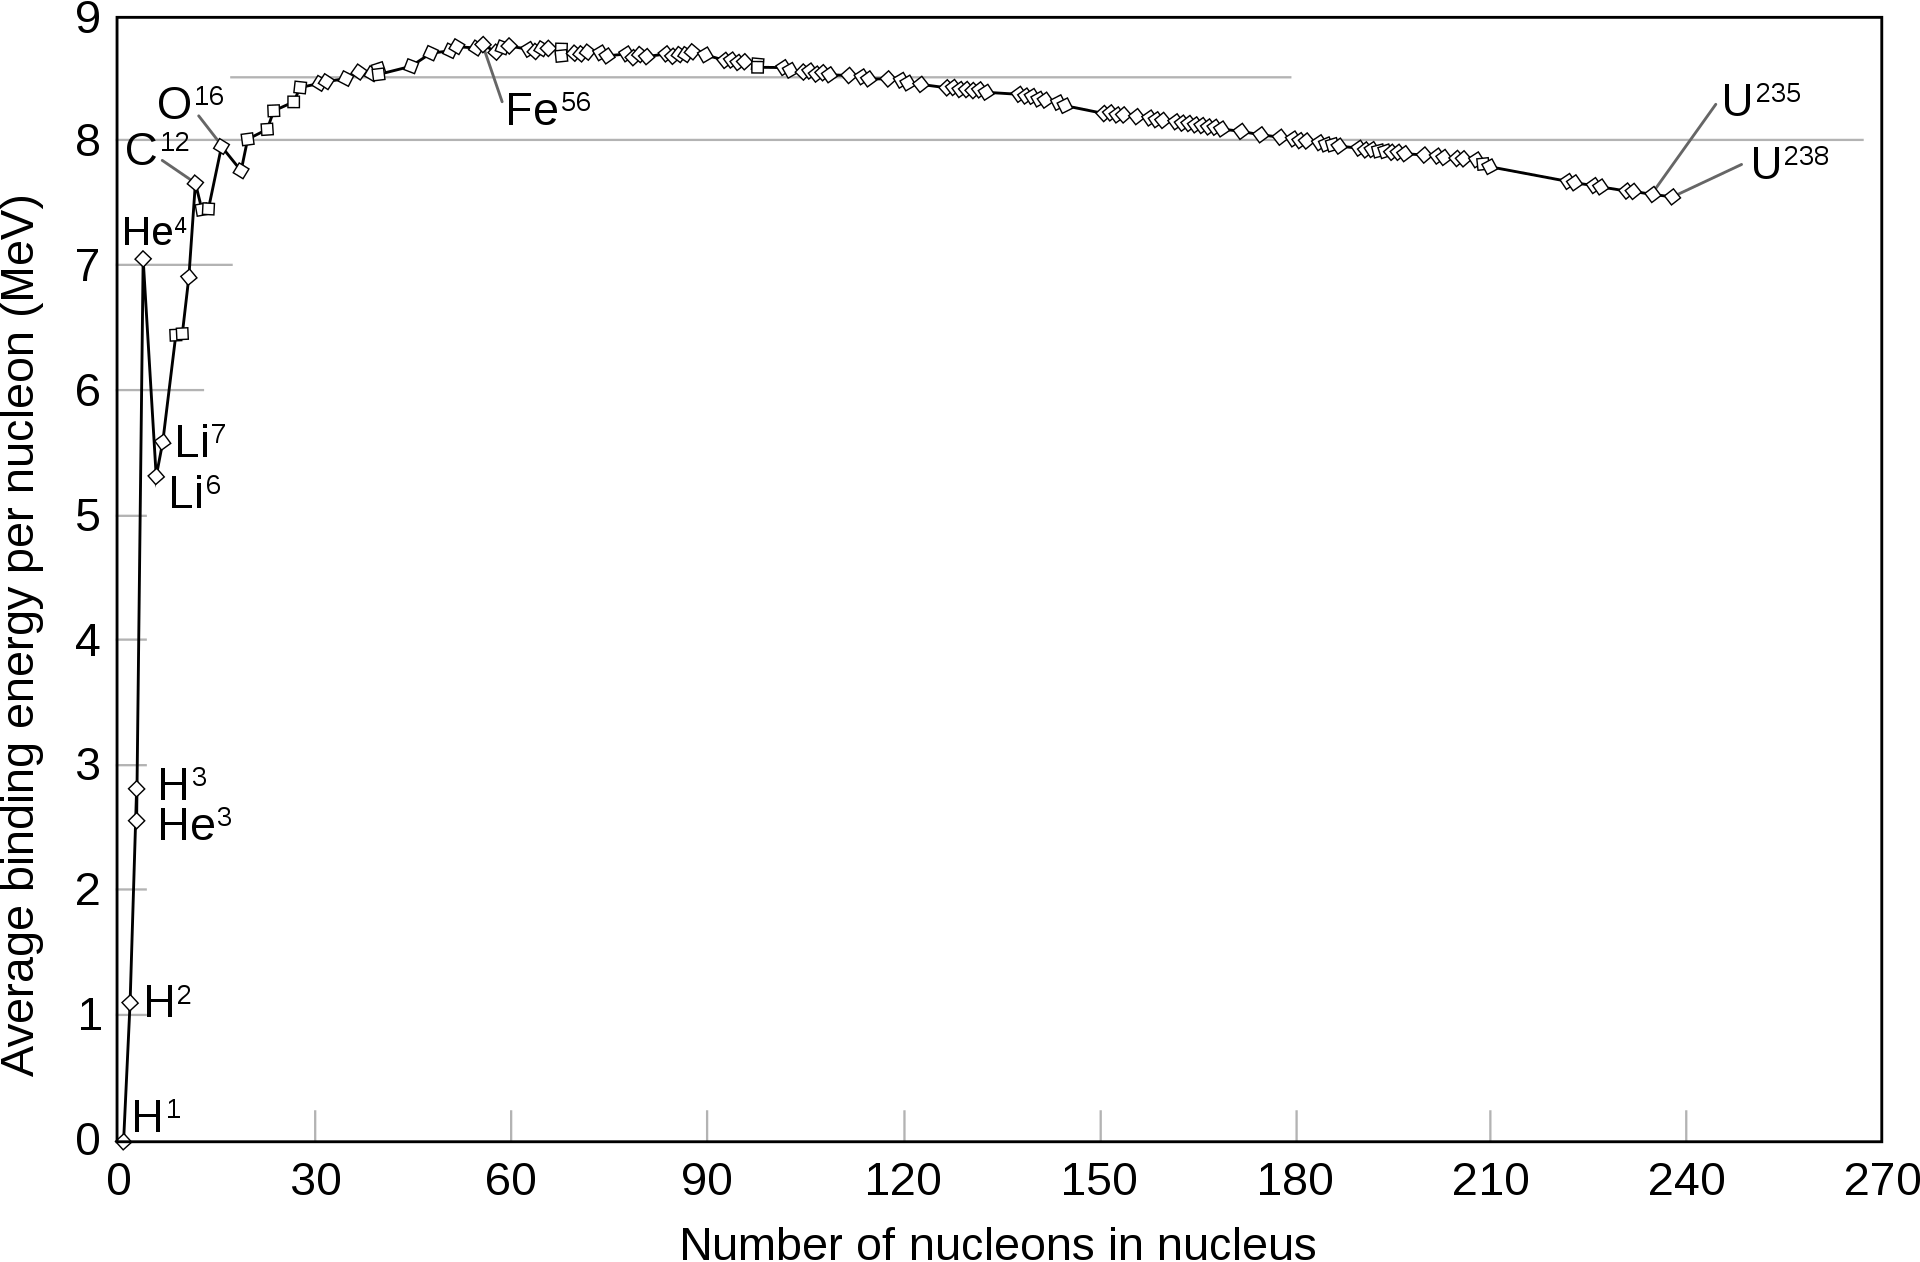
\includegraphics[width=0.5\linewidth]{./figs/fusionEnergy} 

}

\caption{Energy liberated by nuclear fusion. In a star nuclear fusion happens until Iron (Source: Wikipedia)}\label{fig:fusionEnergy}
\end{figure}

Therefore, the star cools down, implodes and subsequently explodes into a supernova (see Figure \ref{fig:supernova}). During the supernova nuclear fusion further occurs towards more heavy elements up to iron (Figure \ref{fig:fusionEnergy}) and these elements are projected in the universe.

\begin{figure}

{\centering 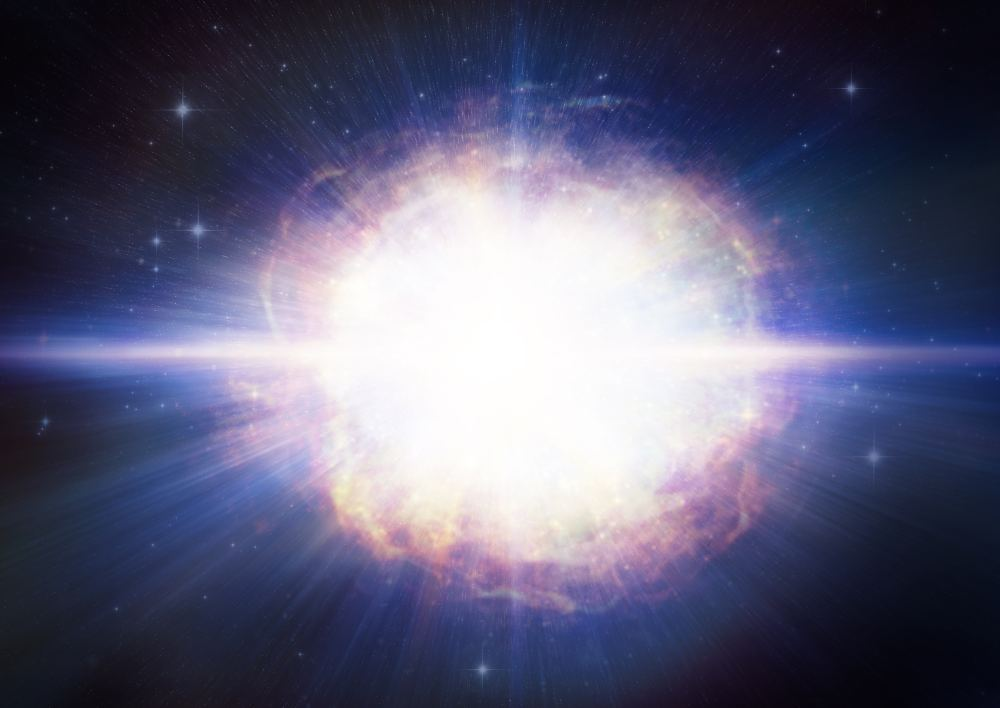
\includegraphics[width=0.5\linewidth]{./figs/hires} 

}

\caption{Supernova of a star (Source:  www.universetoday.com)}\label{fig:supernova}
\end{figure}

A supernova gives rise to new nebula and these will eventually lead to new stars and the whole process begins all over.

Hence, through nuclear fusion in the stars the more heavy atoms have been generated of which the bio-molecules of life are eventually built. So we are built out of cosmic dust!

\newpage

\hypertarget{carbohydrates-in-interstellar-space}{%
\subsection{Carbohydrates in Interstellar Space}\label{carbohydrates-in-interstellar-space}}

Upon nuclear fusion in the stars many different elements are formed. For life, hydrogen, carbon, oxygen, sulfur, phosphorous and nitrogen atoms, among others, are key to compose organic matter.

In interstellar space, carbon reacts spontaneously with other elements to form poly-aromatic carbohydrates (PAHs). This is for instance visible in a photograph of the Cat's paw nebula (Figure \ref{fig:catPawNebula}). In the green regions radiation of hot stars induces fluorescence of PAHs.

\begin{figure}

{\centering 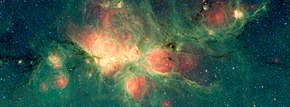
\includegraphics[width=0.5\linewidth]{./figs/orionWithPAH} 

}

\caption{Cat's Paw nebula, in the green regions radiation of hot stars induces fluorescence of PAHs (Source: NASA/JPL-Caltech, Wikipedia)}\label{fig:catPawNebula}
\end{figure}

PAHs were already be generated shortly after the Big Bang. Once they are produced, they are further transformed in interstellar space via hydrogenation (reaction with hydrogen), oxygenation (reaction with oxygen) and other chemical processes to form precursor molecules for amino acids, the building blocks of proteins, and, nucleotides, the building blocks of RNA and DNA. So simple building blocks, molecules that are essential for the chemistry of life are already omnipresent in space.

This together with the fact that chemistry is deterministic under the prevailing physical-chemical conditions let Christian de Duve to formulate his quote that ``Life is an obligatory manifestation of matter, written into the fabric of the universe'' \citep{deDuve2002}.

\hypertarget{genesis-of-life}{%
\section{Genesis of Life}\label{genesis-of-life}}

In a remote corner of our milky way, an average galaxy, an average planet was formed, which we know as our planet Earth.
After the Earth cooled down liquid water was formed. Water is a peculiar molecule and it has the unique feature to form hydrogen bounds between the hydrogen and oxygen atoms of different molecules (see Figure \ref{fig:water}).

\begin{figure}

{\centering 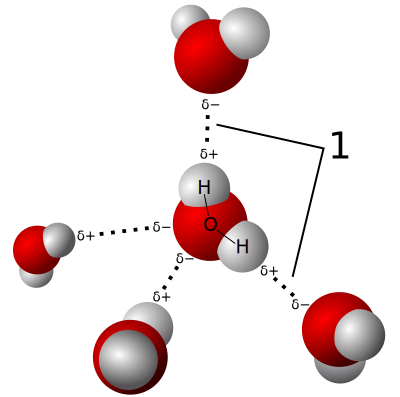
\includegraphics[width=0.25\linewidth]{./figs/3D_model_hydrogen_bonds_in_water} 

}

\caption{Structure of water. A unique feature of water is that it forms hydrogen bounds indicated by (1) (Source: Wikipedia)}\label{fig:water}
\end{figure}

These hydrogen bounds cause water to be liquid at higher temperatures than what we would expect based on the small size of the molecule. It also makes water to freeze with volume increase! Water has its lowest volume while it is liquid at 4°C. These unique features of liquid water are essential for life as we know it.

So on earth unique conditions emerged that made abiogenesis or the \emph{genesis of life} from non-living matter possible. The exact process that led to life is unknown and will probably remain so.
However, a general rationale is displayed in Figure \ref{fig:originOfLife}.

\begin{figure}

{\centering 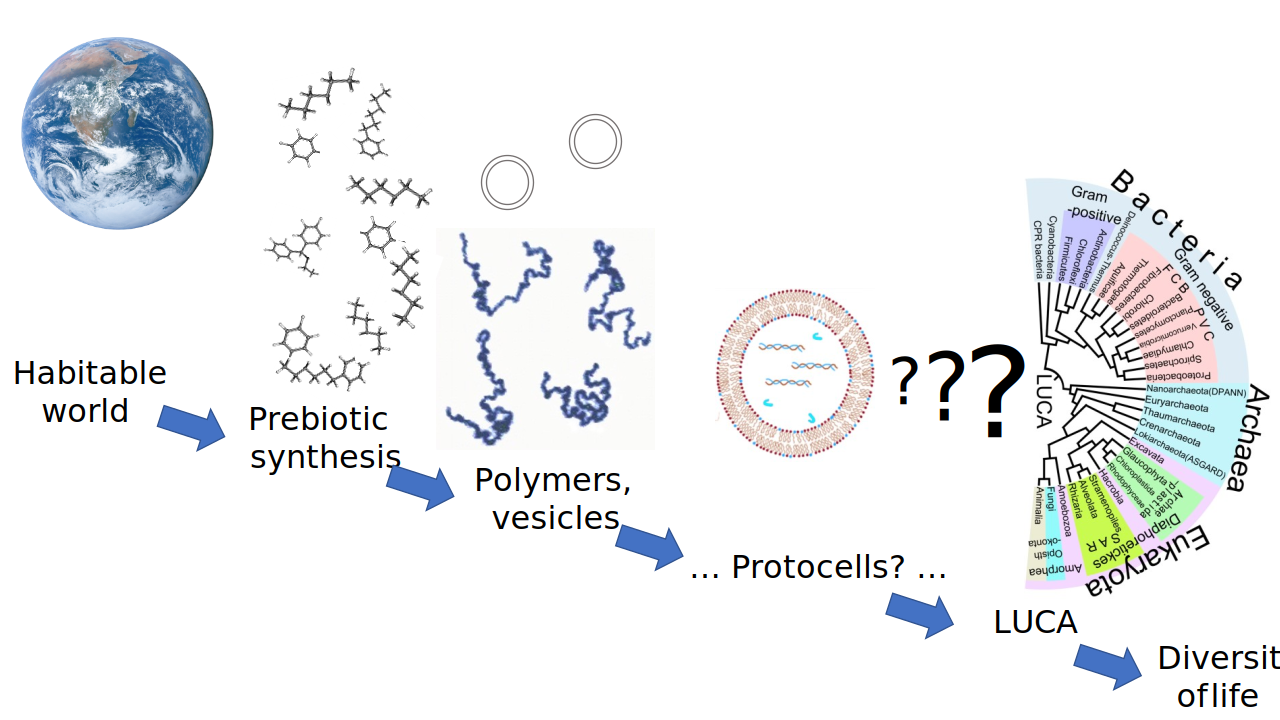
\includegraphics[width=1\linewidth]{./figs/origin_of_life_stages} 

}

\caption{Stages in the origin of life range from well-understood, such as the abiotic synthesis of simple organic molecules, to largely unknown, like the origin of the last universal common ancestor (LUCA) with its complex molecular functionalities. (Source: Chiswick Chap, Wikipedia)}\label{fig:originOfLife}
\end{figure}

Abiogenesis has been initiated by a chemical evolutionary process that gave rise to organic molecules with increasing complexity. It is a general consensus that RNA molecules emerged first from free nucleotides. RNA molecules are known to be catalytic and are carriers of genetic information. They can also replicate themselves under anoxic conditions (in the absence of oxygen) and in the presence of iron, conditions that occurred at young planet Earth (e.g. \citet{Williams2013}). These RNA molecules evolved either alone, the RNA-world hypothesis, or already in conjunction with proteins.

Next, it is assumed that prebiotic molecules, which could self-replicate, were encapsulated by phospholipids, which spontaneously form membrane like structures. This resulted in a protocell with a membrane (see Figure \ref{fig:originOfLife}).
In these protocells a further chemical evolution was possible, separated from the environment, which ultimately led to a self-replicating and self-organizing cell that was built from the four essential type of bio-molecules of life: lipids, carbohydrates, proteins and nucleic acids.

Further biological evolution of these first living cells eventually gave rise to our last universal common ancestor (LUCA).
LUCA must have had at least 355 genes, which all living organisms have in common.
LUCA was anaerobic, living without oxygen, and maintained its hereditary material using DNA, the genetic code, and produced proteins from RNA templates in ribosomes. LUCA retrieved its energy from oceanic volcanic activity in deep sea vents, i.e.~the intensely hot plumes caused by seawater interacting with magma erupting through the ocean floor.

Now, that we introduced the genesis of life, we can focus on the tale of the evolution of LUCA into all species of the tree of life, a process which is also referred to as phylogenesis.

\hypertarget{phylogenesis-and-evolution}{%
\chapter{Phylogenesis and Evolution}\label{phylogenesis-and-evolution}}

In the middle of the model, we see the biological aspect ``phylogenesis'' indicated with the red box in Figure \ref{fig:modelPhylo}, which forms our focus in this chapter.

\begin{figure}

{\centering 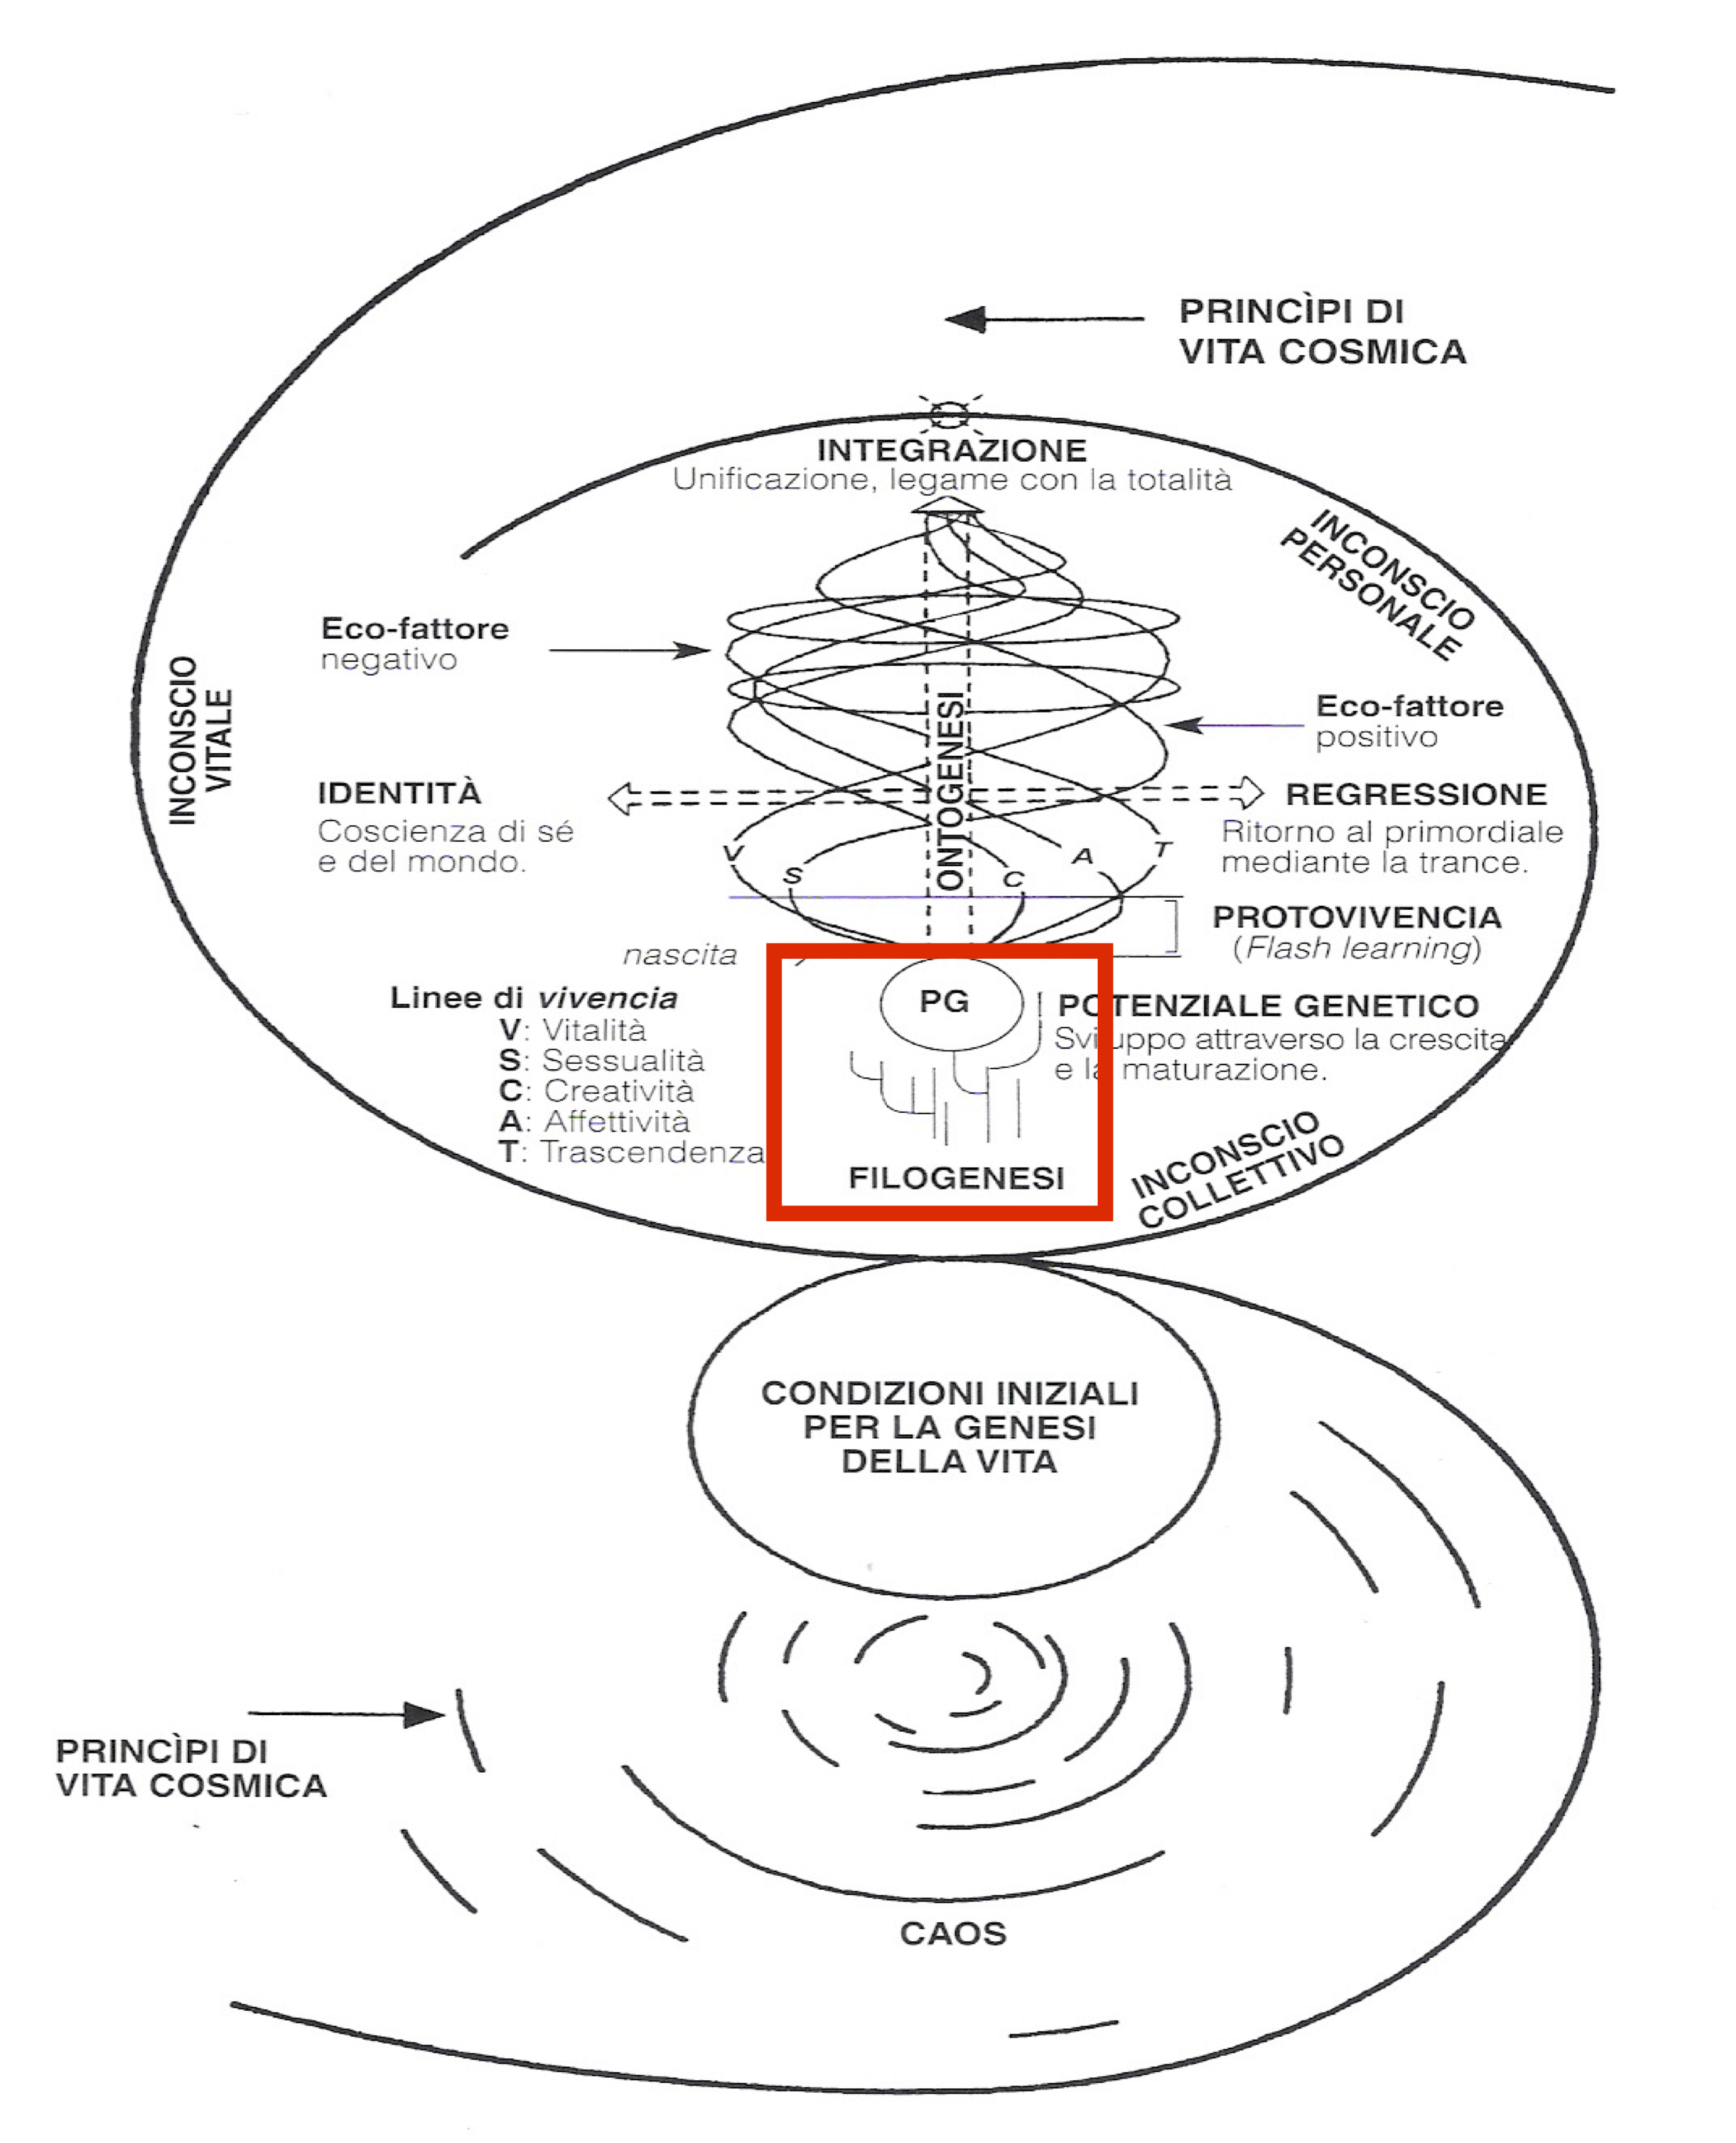
\includegraphics[width=0.5\linewidth]{./figs/biologischeAspectenBiodanzaDeelII} 

}

\caption{Model of Biodanza and Phylogenesis}\label{fig:modelPhylo}
\end{figure}

\hypertarget{phylogenesis}{%
\section{Phylogenesis}\label{phylogenesis}}

All species evolved from the same ancestral population of cells.
This is also referred to as the same Last Universal Common Ancestor (LUCA).
In the tree of life the evolutionary relations are summarized between different organisms (and groups of organisms). All living beings eventually can be traced back to the last universal common ancestor who is located at the root of the tree, see Figure \ref{fig:treeOfLifeBis}.

\begin{figure}

{\centering 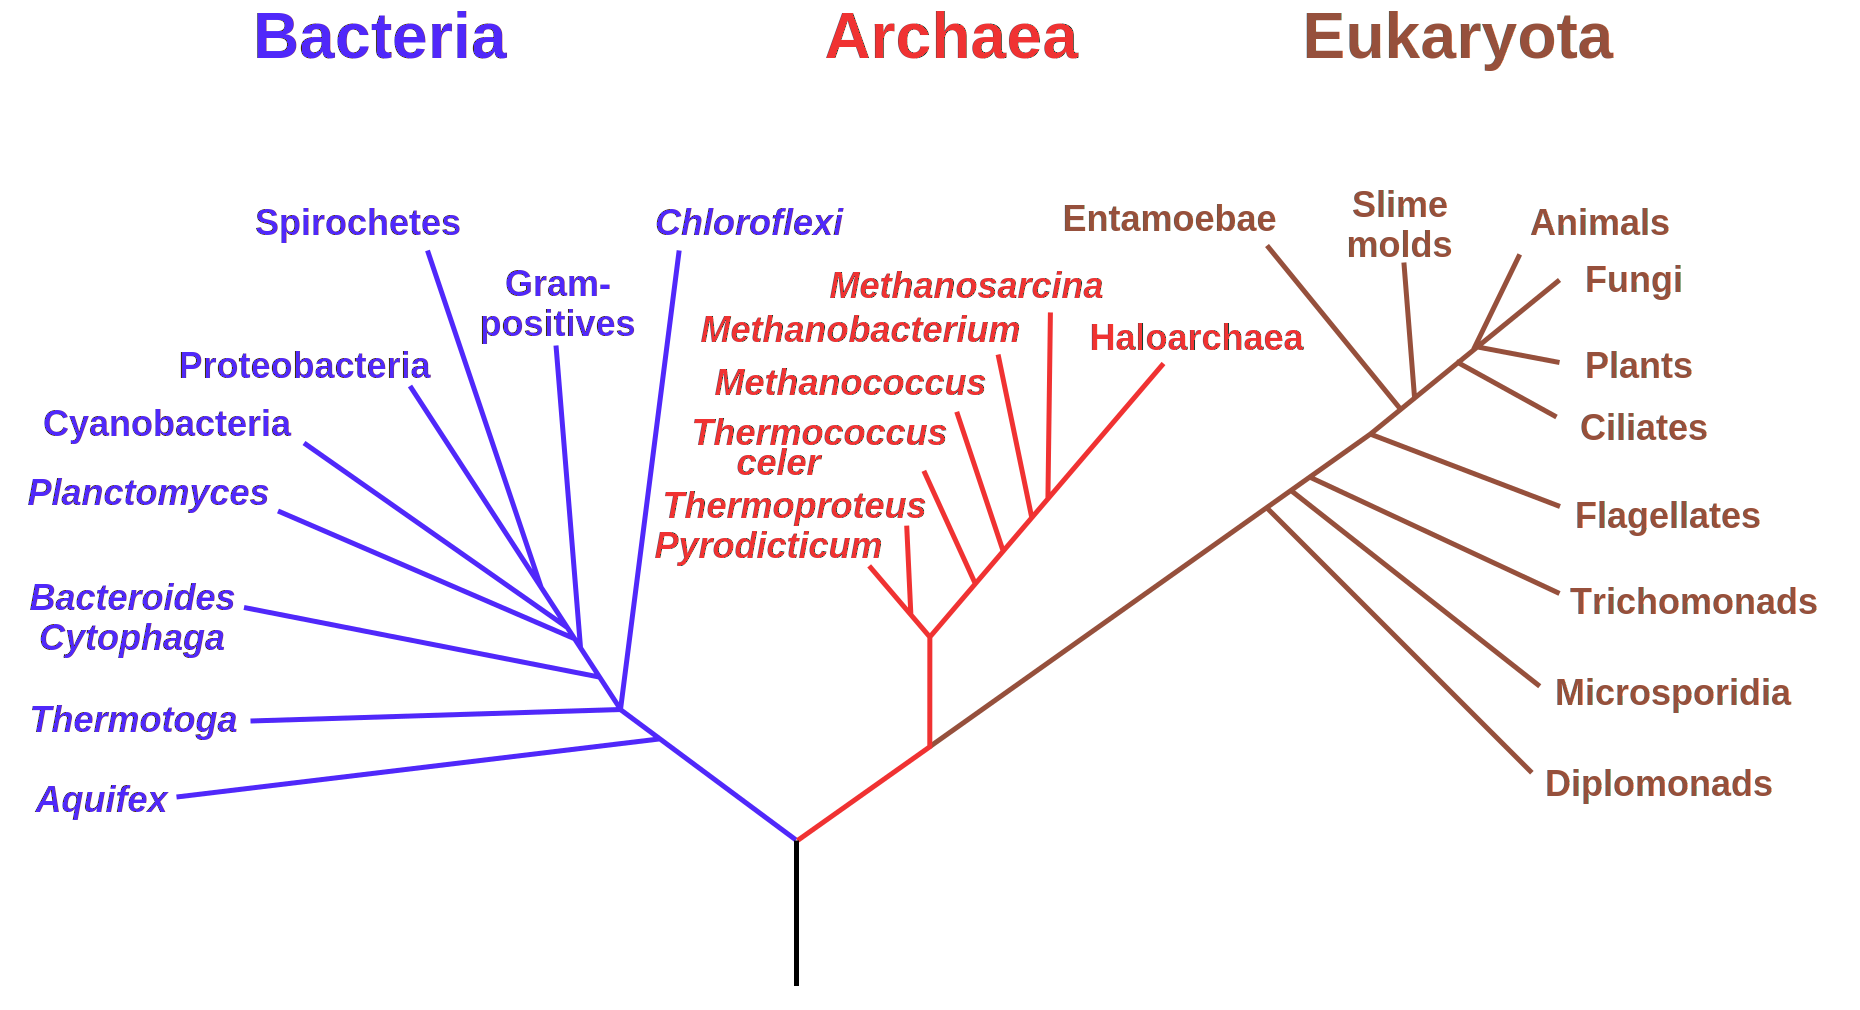
\includegraphics[width=1\linewidth]{./figs/Phylogenetic_tree} 

}

\caption{The tree of life is one of the most important organizing principles in biology. It shows the evolutionary relationships among different organisms and that all living beings eventually can be traced back to the last universal common ancestor who is located at the root of the tree (Source: wikipedia)}\label{fig:treeOfLifeBis}
\end{figure}

Phylogenesis is the process of the origin of all species from the tree of life from LUCA.

Rolando Toro refers to the origin of species and adaptation to the environment as evolutionary differentiation.

\hypertarget{timescale}{%
\subsection{Timescale}\label{timescale}}

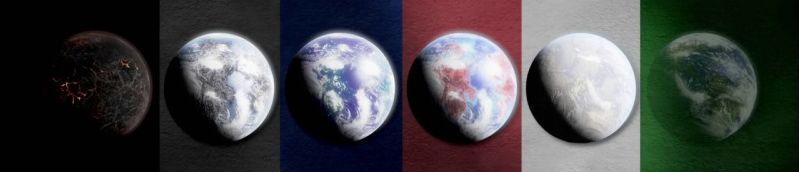
\includegraphics{./figs/liferockystartstrip.jpeg}

\begin{longtable}[]{@{}llllll@{}}
\toprule()
4.5 BYA & 4.3 BYA & 3.8 BYA & 3.5 BYA & 540 MYA & 520 MYA \\
\midrule()
\endhead
& & & & & \\
\bottomrule()
\end{longtable}

(Source: naturedocumetaries.org)

At its origin about 4.5 Billion Years Ago (BYA) the Earth was black, a hot basalt rock and dust in a cold vacuum.
As the Earth cooled down she became Grey Earth (4.3 BYA) as she was mainly covered by granite and rocks. Another 500 million years later she was covered with liquid water: Blue Earth (3.8 BYA).

In only 300 million years she radically changed into Red Earth (3.5 BYA) due to life. Indeed, cyanobacteria emerged that can do photosynthesis and produce oxygen, a very reactive molecule. This led all free iron in the ocean to precipitate as iron oxide or rust (red). There was an explosion of the number of minerals, they went from approximately 250 to more than 5000 mineral species. Oxygen also caused a mass extinction because only few organisms could cope with its highly reactive nature. The coming 3 billion years life on Earth stayed relatively similar.

Around 540 MYA Earth was struck by a large ice age, White Earth.
Again leading to a mass extinction due to the cold. However, volcanic activity came to the rescue by producing greenhouse gasses and an atmosphere that could retain more heat.

In less than 20 million years (MY) Earth radically changed again and turned into Green Earth (520 MYA). In only 20 MY there was an explosion of life, and life suddenly evolved from unicellular to more complex multicellular forms.

\hypertarget{change-point-genesis-of-eukaryotic-cells}{%
\subsection{Change Point: Genesis of Eukaryotic Cells}\label{change-point-genesis-of-eukaryotic-cells}}

The change point that made the origin of multicellular species possible was the genesis of eukaryotic cells.

There are two archetypes of cells:

\begin{itemize}
\tightlist
\item
  Prokaryota, simple cells of a size of 0.1 to 5.0 \(\mu m\) with DNA that is lying freely in the cell cytosol (the fluid in the cell), see Figure \ref{fig:prokaryotaCell} and
\end{itemize}

\begin{figure}

{\centering 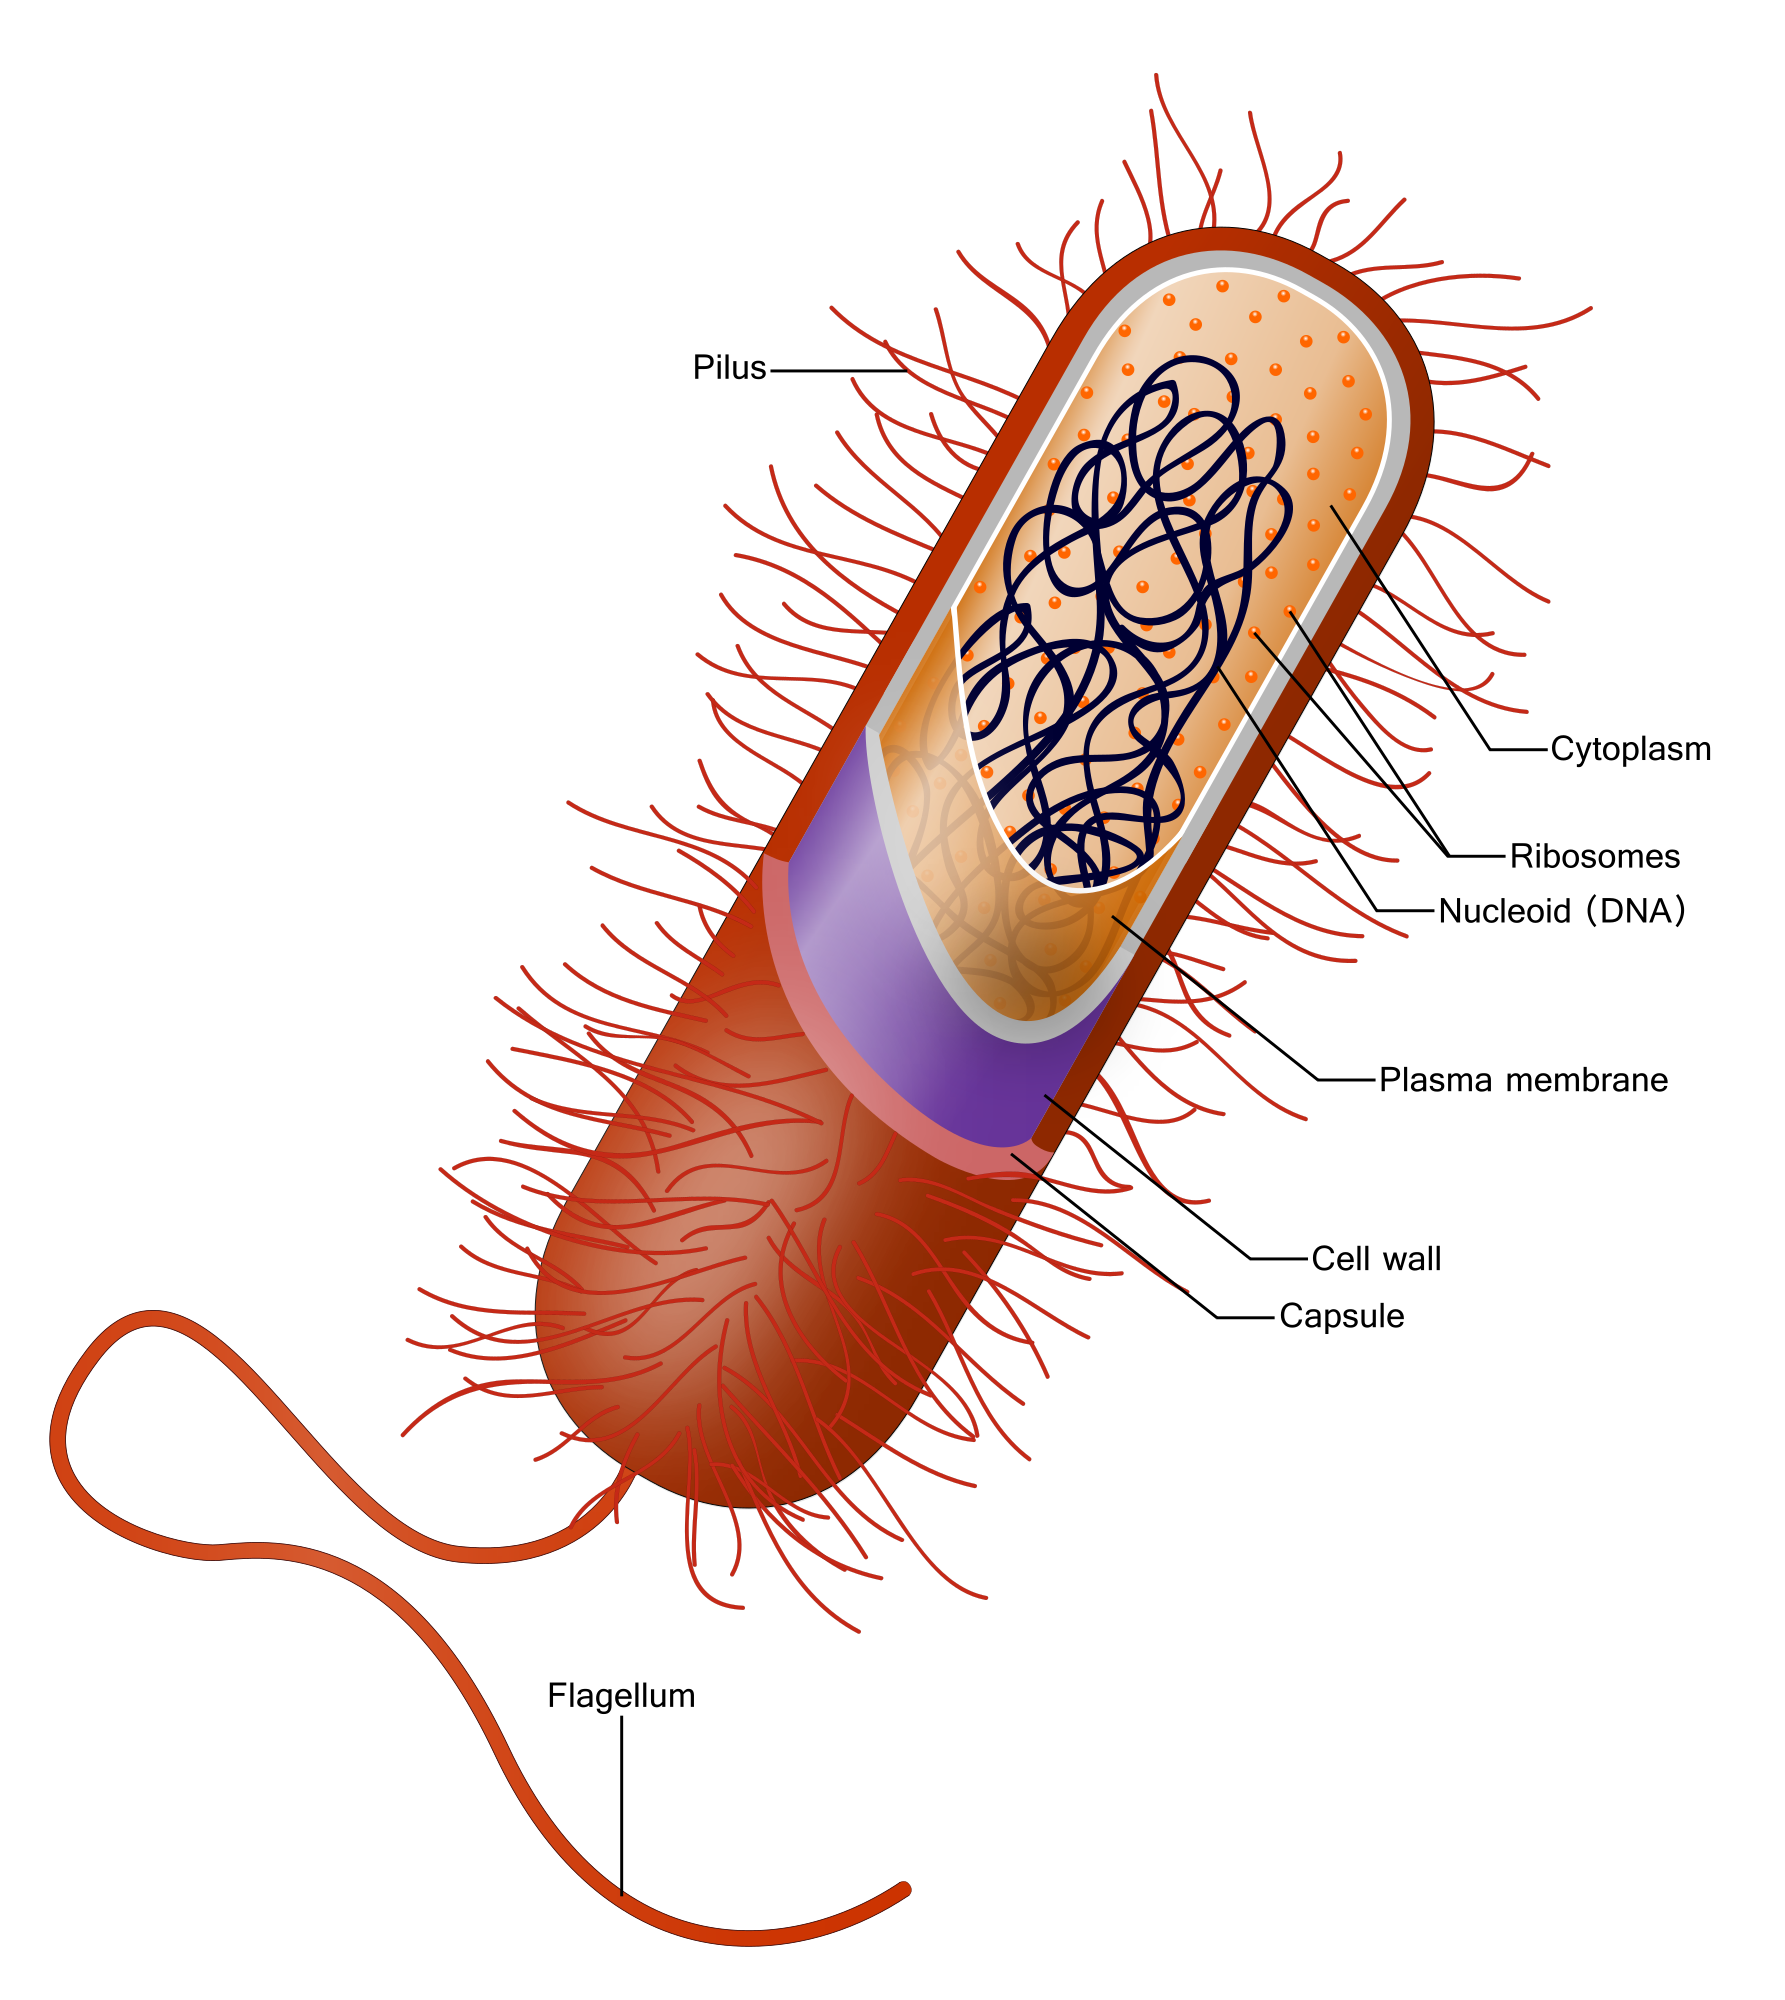
\includegraphics[width=0.5\linewidth]{./figs/prokaryoteCell} 

}

\caption{Diagram of a typical prokaryotic cell. The cell is simple, the DNA is lying free in the cell (Source: Ali Zifan, Wikipedia)}\label{fig:prokaryotaCell}
\end{figure}

\begin{itemize}
\tightlist
\item
  Eukaryota are larger and more complex cells, 10-100 \(\mu m\) in size. They have a variety of internal membrane-bound structures, called organelles, and a cytoskeleton, which play an important role in defining the cell's organization and shape. Eukaryotic DNA is stored in chromosomes. A chromosome is a long DNA molecule that is stored in a compact form. A chromosome contains a part or all of the genetic material of an organism. Human cells have 46 chromosomes, i.e.~23 chromosome pairs. Each pair consists of one copy from our biological mother and one from our biological father. The chromosomes are located in the cell nucleus, which is the organelle maintaining the integrity of chromosomes and thus of our genes, and is controlling the activities of the cell by regulating gene expression. The nucleus can, therefore, be viewed as the control center of the cell, see \ref{fig:animalCell} and \ref{fig:plantCell}.
\end{itemize}

\begin{figure}

{\centering 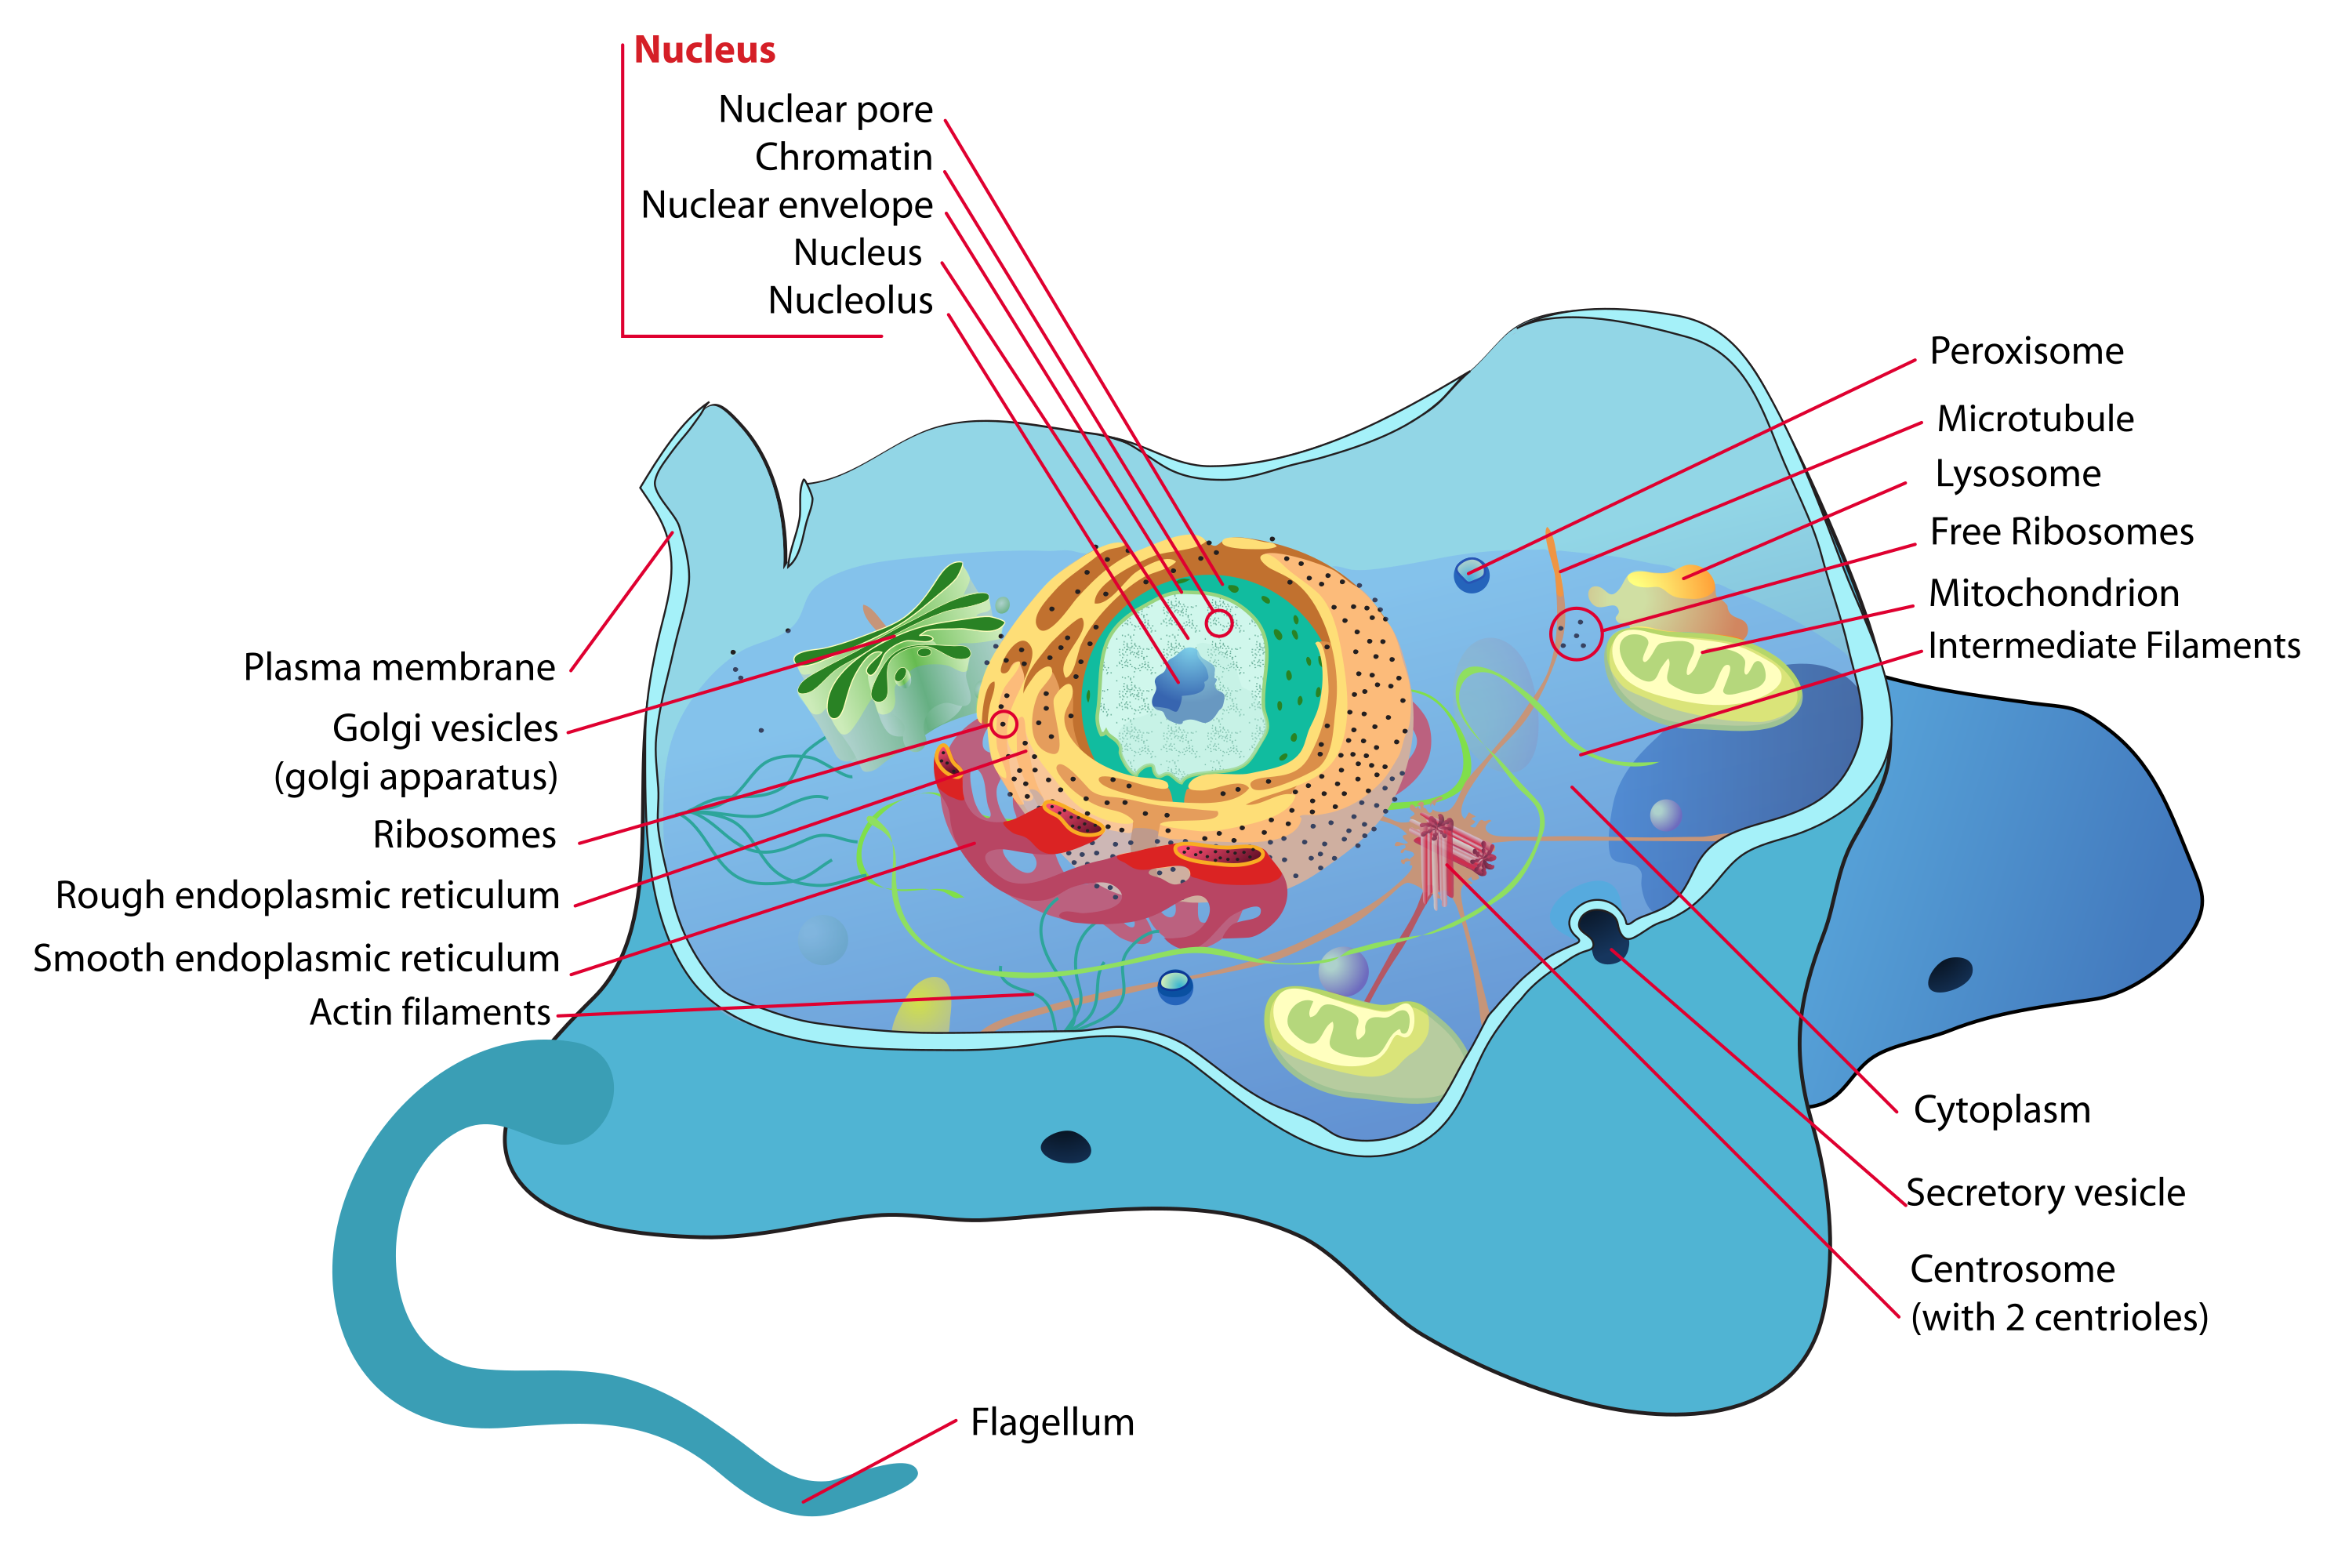
\includegraphics[width=0.5\linewidth]{./figs/animalCell} 

}

\caption{Diagram of a typical animal cell. Animal cells are eukaryotic cells. They are typically much larger than those of prokaryotas. They have a variety of internal membrane-bound structures, called organelles, and a cytoskeleton, which play an important role in defining the cell's organization and shape. Eukaryotic DNA is divided into chromosomes, that are located in the cell nucleus, which is the organelle maintaining the integrity of genes and controlling the activities of the cell by regulating gene expression. (Source: Mariana Ruiz Villarreal, Wikipedia)}\label{fig:animalCell}
\end{figure}

\begin{figure}

{\centering 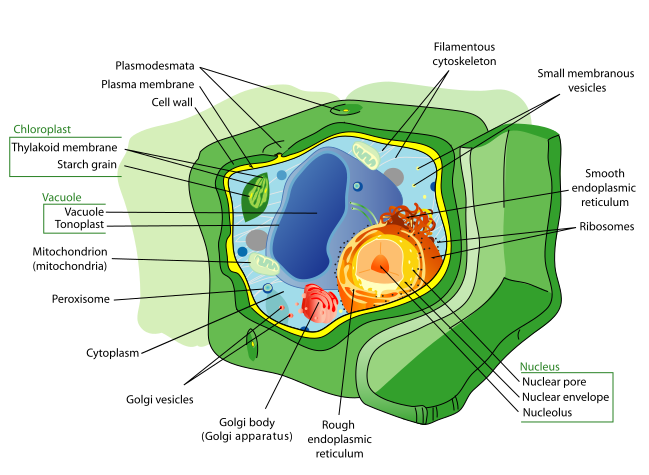
\includegraphics[width=0.5\linewidth]{./figs/plantCell} 

}

\caption{Diagram of a typical plant cell. Animal cells are eukaryotic cells. They are typically much larger than those of prokaryotas. They have a variety of internal membrane-bound structures, called organelles, and a cytoskeleton, which play an important role in defining the cell's organization and shape. Eukaryotic DNA is divided into chromosomes, that are located in the cell nucleus, which is the organelle maintaining the integrity of genes and controlling the activities of the cell by regulating gene expression. Plant cells also have a cell wall and chloroplasts that can perform photosynthesis. (Source: Mariana Ruiz Villarreal, Wikipedia)}\label{fig:plantCell}
\end{figure}

From 3.5 BYA - 520 MYA we only find prokaryota cells in fossils.
Eukaryotic cells are believed to be generated by endosymbiosis, i.e.~a symbiotic relationship where one organism lives inside the other, which is beneficial for both organisms.

The process of endosymbiosis that led to eukaryotic cells is displayed in Figure \ref{fig:endosymbiosis}.

\begin{figure}

{\centering 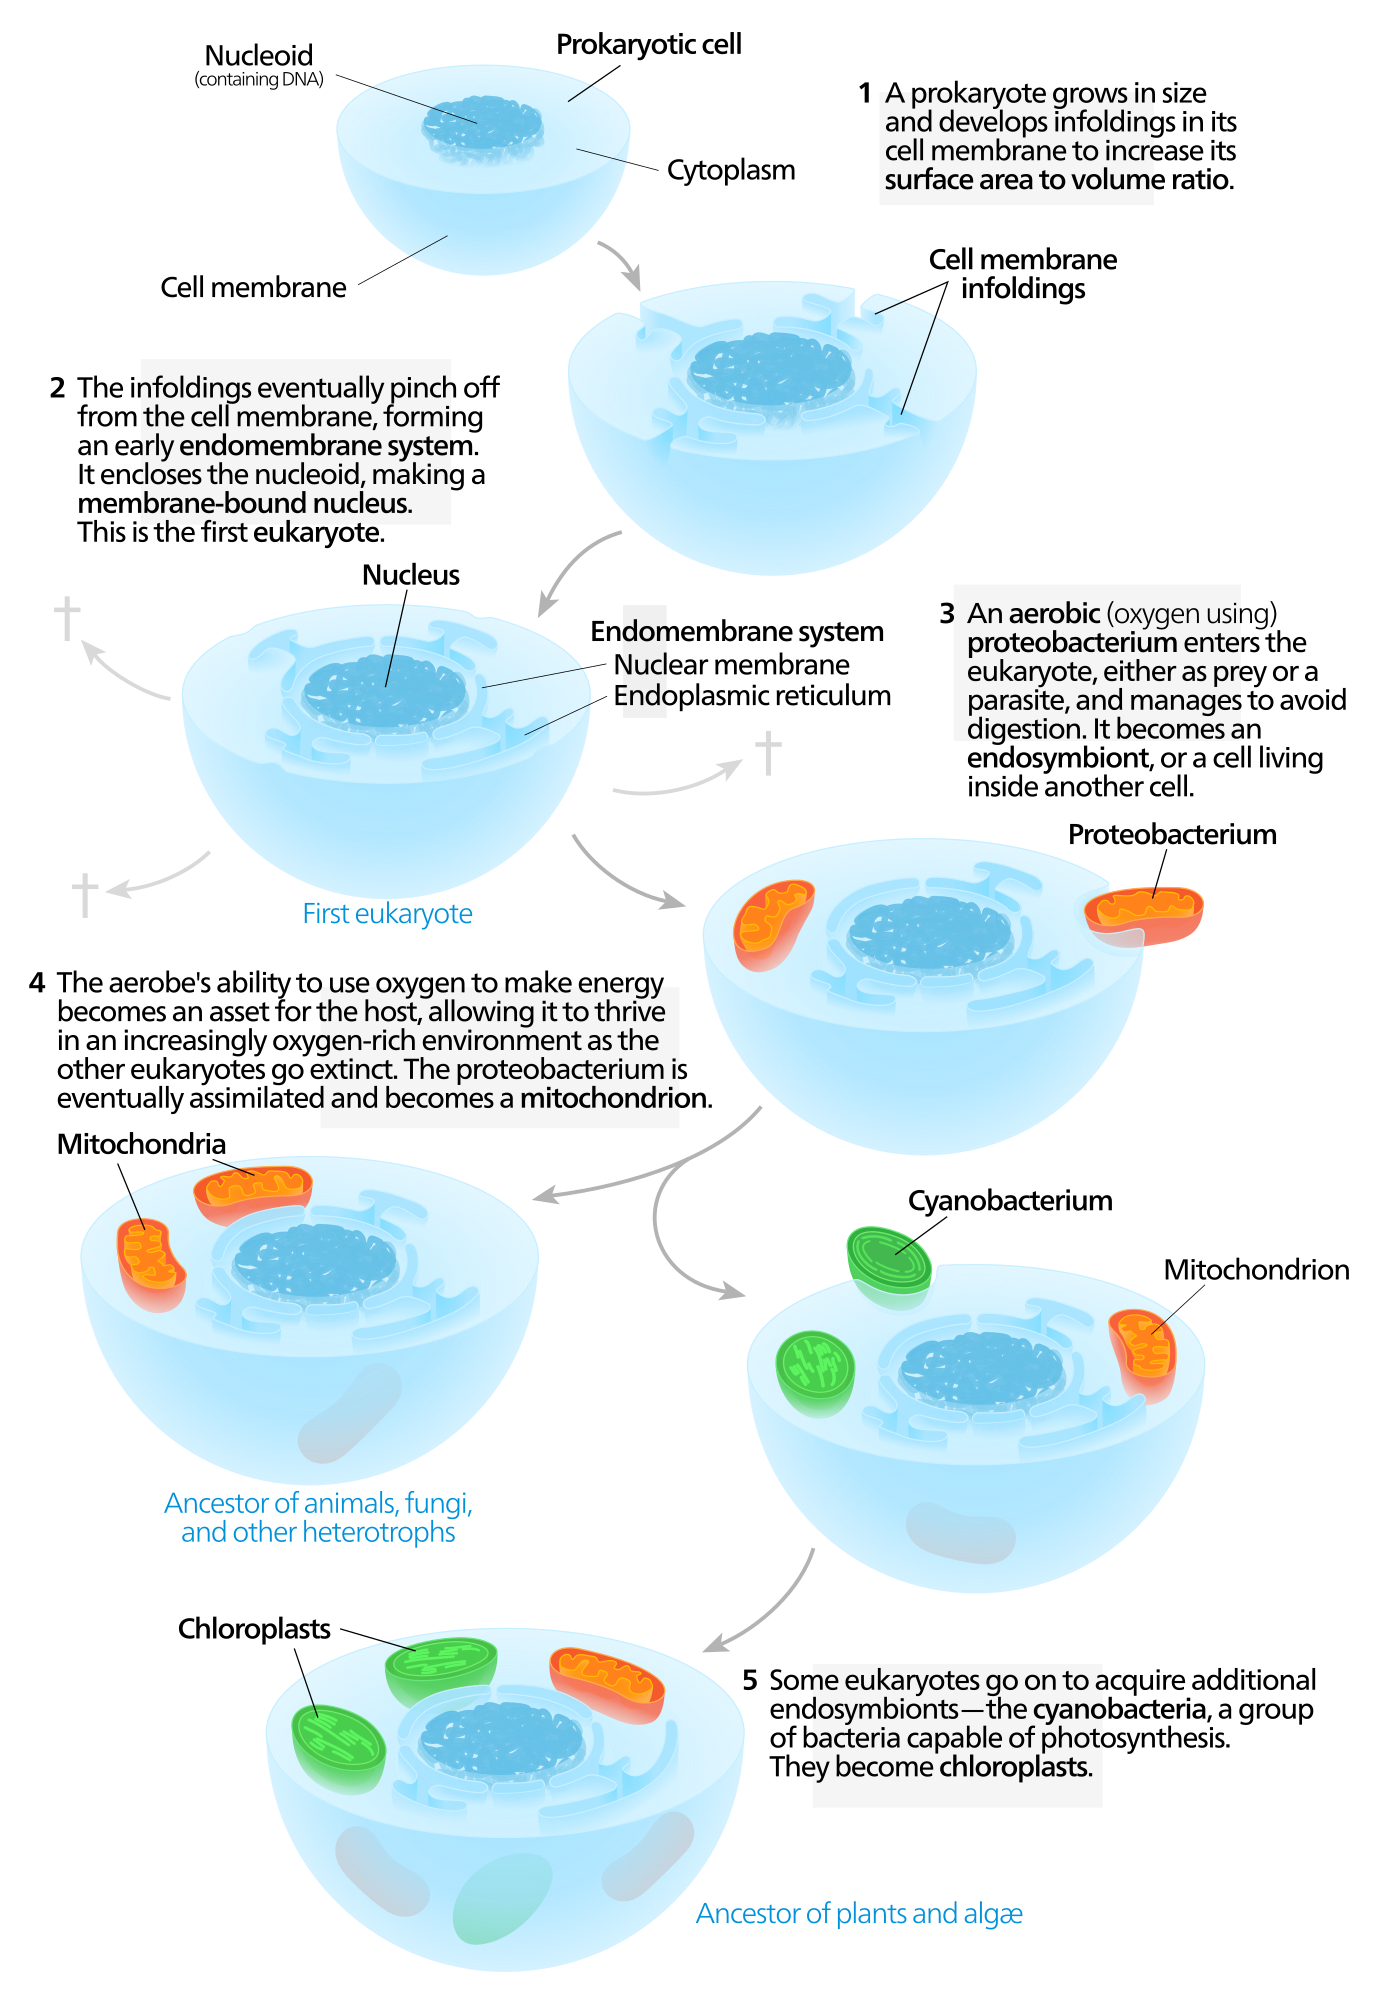
\includegraphics[width=0.8\linewidth]{./figs/endosymbiosis} 

}

\caption{Genesis of eukaryotic cells (Source: wikipedia)}\label{fig:endosymbiosis}
\end{figure}

First a prokaryotic cell is assumed to grow and to generate membrane systems inside the cell, which gave rise to the formation of the nucleus. At a certain point of time a proteobacterium that could use oxygen for respiration must have been ingested, which managed to avoid digestion. The two cells started with an endosymbiotic relation.

The proteobacterium provided the cell with additional energy and the host cell fed the proteobacterium with nutrients. This gave the endosymbiotic pair to ability to grow further in size and to thrive in the oxygen rich environment of planet Earth.

The proteobacterium gradually handed over a number of its genes to the cell nucleus, and became under regulation of the nucleus. It eventually evolved to mitochondria, the organelles that are the energy plants of a cell. So, we inherit more from mother than father: we inherit our cell structure and energy system from mother side through her egg cell.

In plant cells, a second endosymbiotic event must have occurred with eukaryotic cells and cyanobacteria. The cyanobacteria then evolved in a similar way into chloroplasts, which give plants the ability for photosynthesis and led them become the most successful life form of the globe.

Other key differences between Prokaryota and Eukaryota are in terms of their reproduction.
For Prokaryota that only takes place by cell division. A mutation in the DNA is thus fixed in all daughter cells. While nearly all Eukaryota have a phase of sexual reproduction. They are diploid organisms, i.e.~they have two copies of each gene, one from fathers' and mothers' side. This enables successive mutations to be made in one copy because another functional copy of the gene is available. Moreover during sexual reproduction recombination of chromosomes occurs, i.e.~reshuffling of paternal and maternal genes, which leads to much more variation.

The Eukaryota further evolved in protists, which are unicellular organisms, fungae, plants and animals.

\newpage

\hypertarget{evolution}{%
\section{Evolution}\label{evolution}}

How thus the evolution of LUCA to all species of the tree of life occurred?
Evolution is largely driven by variability and selection.

\hypertarget{variability-and-selection}{%
\subsection{Variability and Selection}\label{variability-and-selection}}

Variation occurs, among others, through errors in the copying of DNA for cell division of prokaryotic cells and gamete production for eukaryotic cells (see Figure \ref{fig:dnaPolymerase}).

\begin{figure}

{\centering 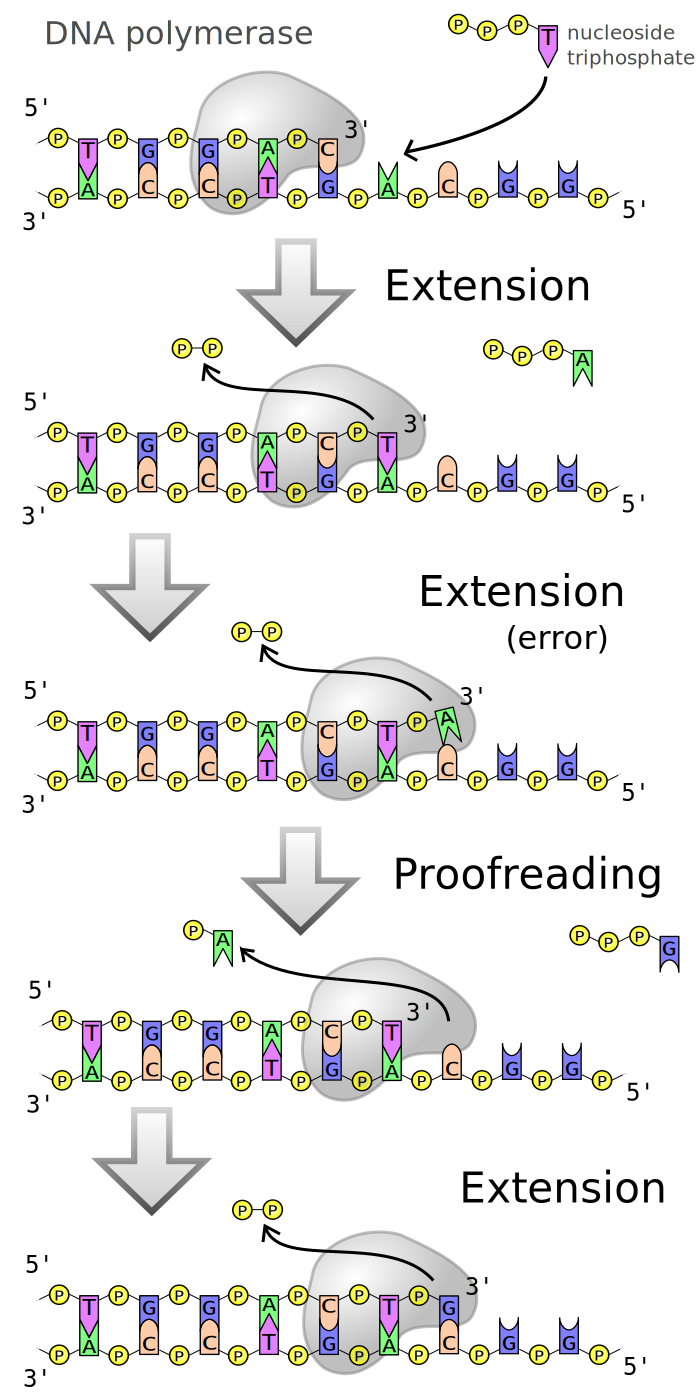
\includegraphics[width=0.45\linewidth]{./figs/DNA_polymerase} 

}

\caption{Copying of DNA by DNA-polymerase. DNA polymerase extends a DNA strand by incorporating a complementary nucleoside-tri-phosphate and splitting two of the three phosphate groups  (Note again the link between energy and information). Errors are often corrected by proofreading. However, some of the errors remain.}\label{fig:dnaPolymerase}
\end{figure}

The error margin of DNA replication is 1 error per billion base pairs that are copied, which can lead to point mutations. Note, that we humans have a genome size of about 6.4 billion base pairs.

Other sources of variability are

\begin{itemize}
\tightlist
\item
  Insertions or deletions, i.e.~base pairs that are added or removed, respectively.
\item
  Recombination, reshuffling of genetic traits, e.g.~during sexual reproduction
\end{itemize}

Most mutations are neutral, i.e.~the mutated codon encodes for the same amino acid. Neutral mutations can be used as a molecular/genetic clock to tell how far apart two species are in an evolutionary sense.

But, mutations are not always neutral! For instance, sickle cell anemia is caused by one point mutation in hemoglobin (see Figure \ref{fig:sickleCell1} and \ref{fig:sickleCell2}). A thymine is mutated to an adenine, which results in a codon that encodes for the amino acid valine instead of glutamic acid. This causes dramatic changes to the 3D structure of the hemoglobin protein and causes a deformation of the red blood cells from a round to sickle shape, which leads to anemia.

Why does this mutation remain? It mainly occurs in Africa because sickle cell anemia also makes affected individuals resistant against malaria, which gives them a evolutionary competitive advantage despite their anemia. However, offspring that inherits the mutation of both parents is not viable.

\begin{figure}

{\centering 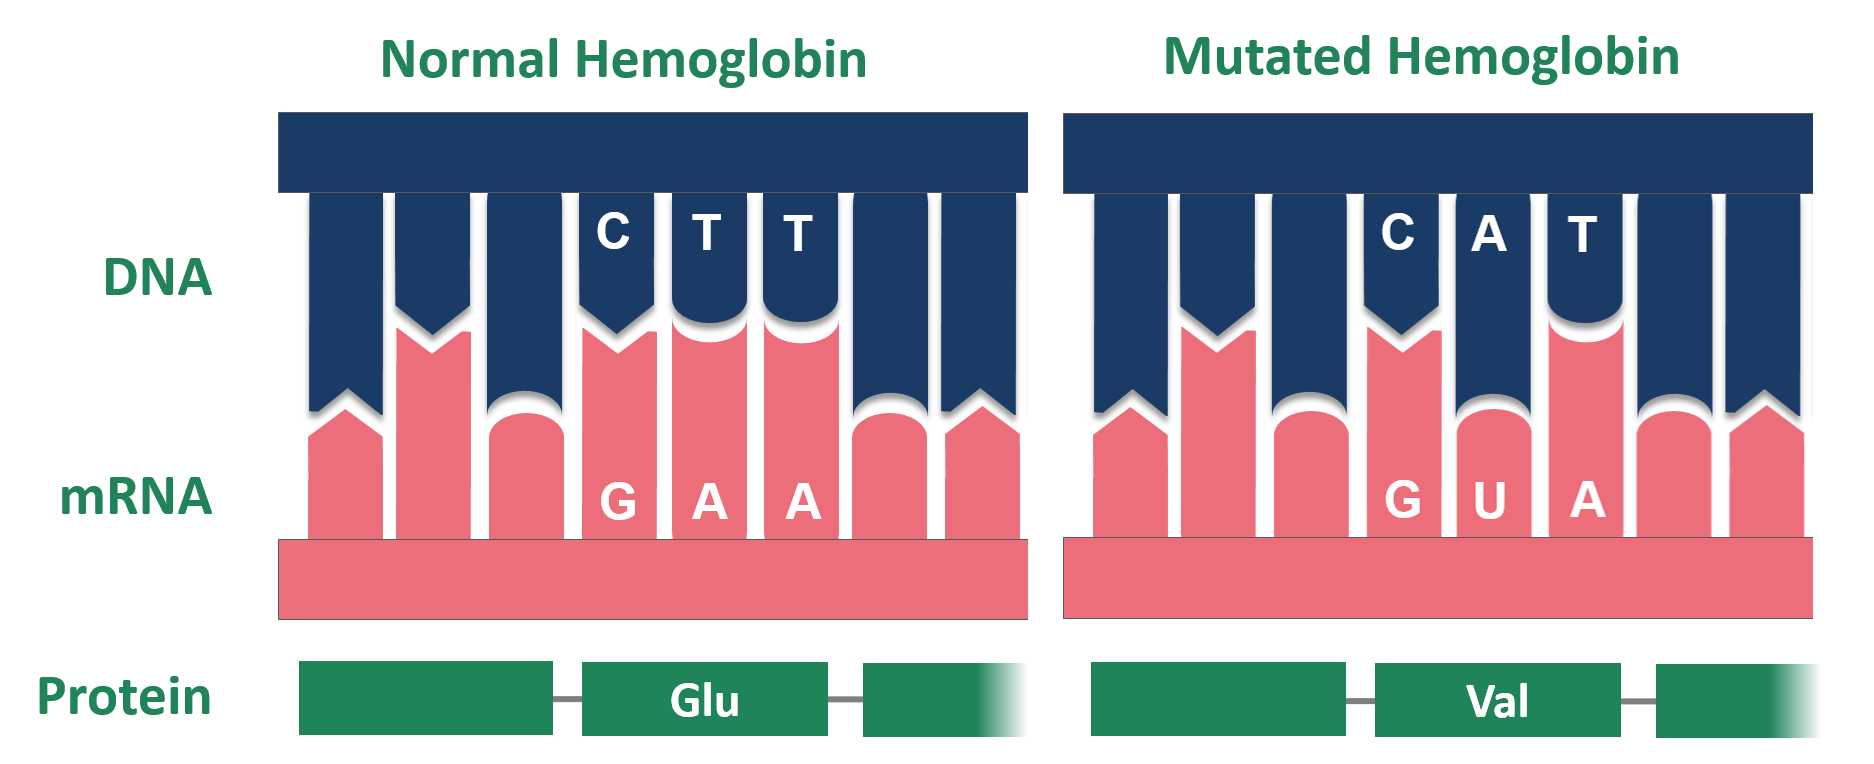
\includegraphics[width=0.45\linewidth]{./figs/sickleCellWikipedia2} 

}

\caption{Mutation of Hemoglobin in patients with sickle cell anemia (Source: Wikipedia)}\label{fig:sickleCell1}
\end{figure}

\begin{figure}

{\centering 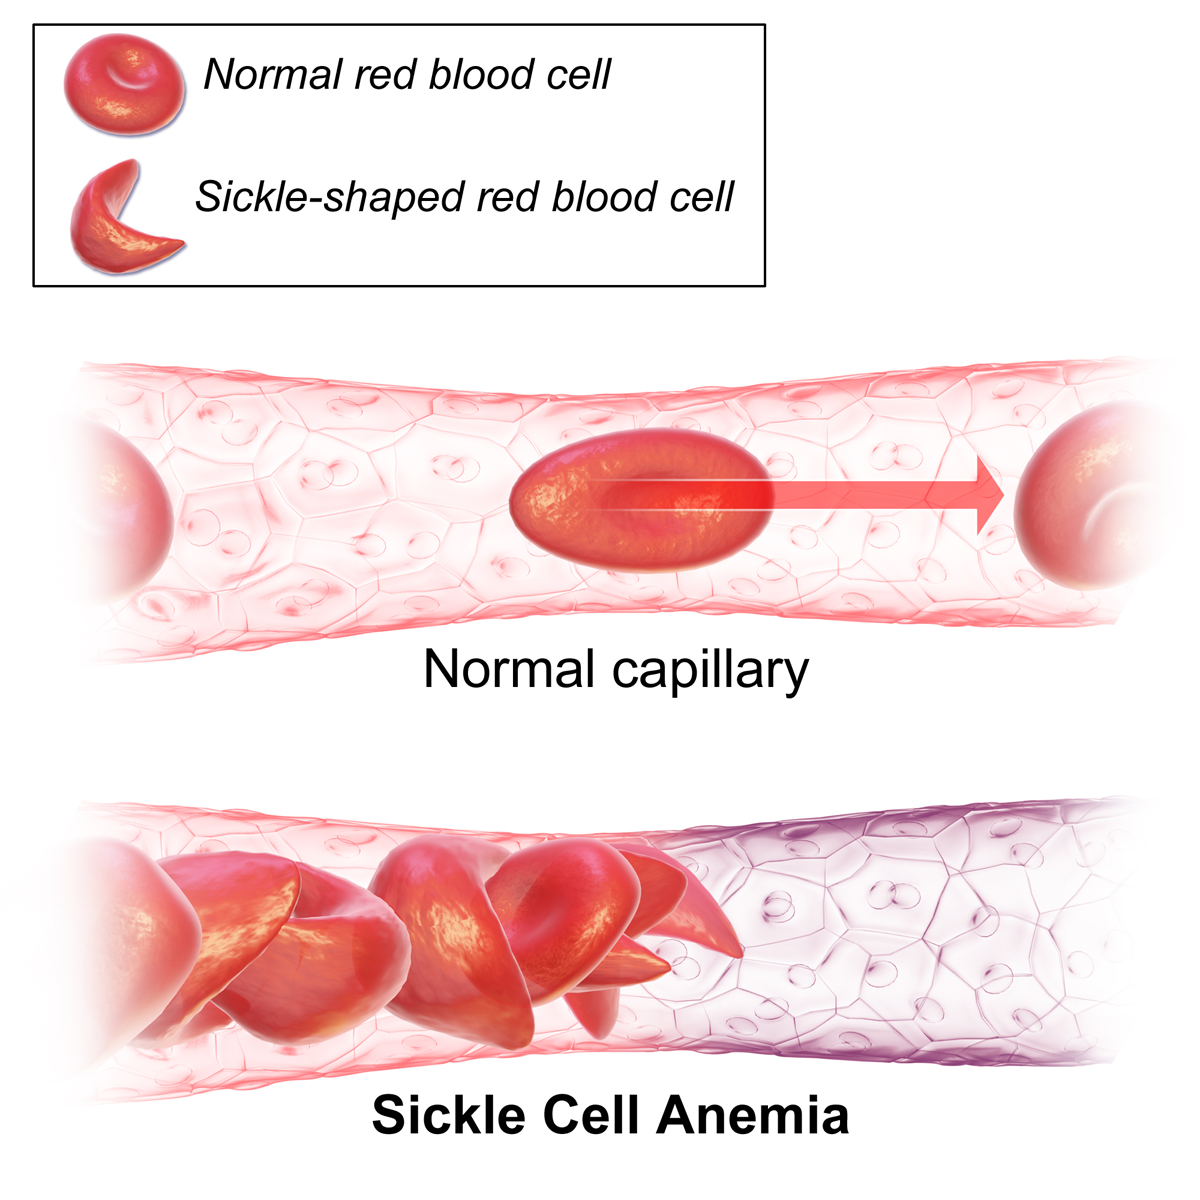
\includegraphics[width=0.45\linewidth]{./figs/Sickle_Cell_Anemia_wiki3} 

}

\caption{Deformed red blood cells in patients with sickle cell anemia (Source: Wikipedia)}\label{fig:sickleCell2}
\end{figure}

\hypertarget{evolution-1}{%
\subsection{Evolution}\label{evolution-1}}

Evolution is a natural process that forms the basis of the origin of species (bacteria, fungi, plants, animals).

It is driven by two opposing forces: variation and selection

Variation occurs by spontaneous copy errors in genetic code or mutations, among others.

Selection occurs upon ecofactors. Is a mutation beneficial or harmful for a particular organism in its specific environment.
The odds on fixation of the mutation thus depends on the reproductive success.

The process of genetic variation and selection can eventually lead to new species upon many generations.

\hypertarget{genetic-drift}{%
\subsection{Genetic Drift}\label{genetic-drift}}

Another important process for the origin of species is genetic drift. This are random fluctuations of alleles, which are particular sequence variants of a gene. Genetic drift is particularly strong in small populations. As opposed to selection it is not adaptive.

New species will thus originate more quickly when a small fraction of the population gets isolated in a new environment.

\hypertarget{horizontal-gene-transfer}{%
\subsection{Horizontal Gene Transfer}\label{horizontal-gene-transfer}}

A last process that introduces variation is horizontal gene transfer, in example non-sexual transfer of genetic information between two distinct organisms.

This is very common between Prokaryota, i.e.~eubacteria and archaea bacteria, think on the super bugs in hospitals that acquired resistance to multiple antibiotics. It also occurs between Eukaryota. Mainly in protists, which are unicellular organisms with a nucleus. As well as between Prokaryota on the one hand and Eukaryota on the other hand.

\hypertarget{teleonomy}{%
\subsection{Teleonomy}\label{teleonomy}}

The term teleonomy means that evolution only has the primitive goal to maintain and reproduce the species, and, that it thus has no purpose or direction.

When complex organs and organisms originate it might seem as if there is a direction or purpose, but, that is not the case! A good example is the development of an eye, see Figure \ref{fig:evolutionEye}.

\begin{figure}

{\centering 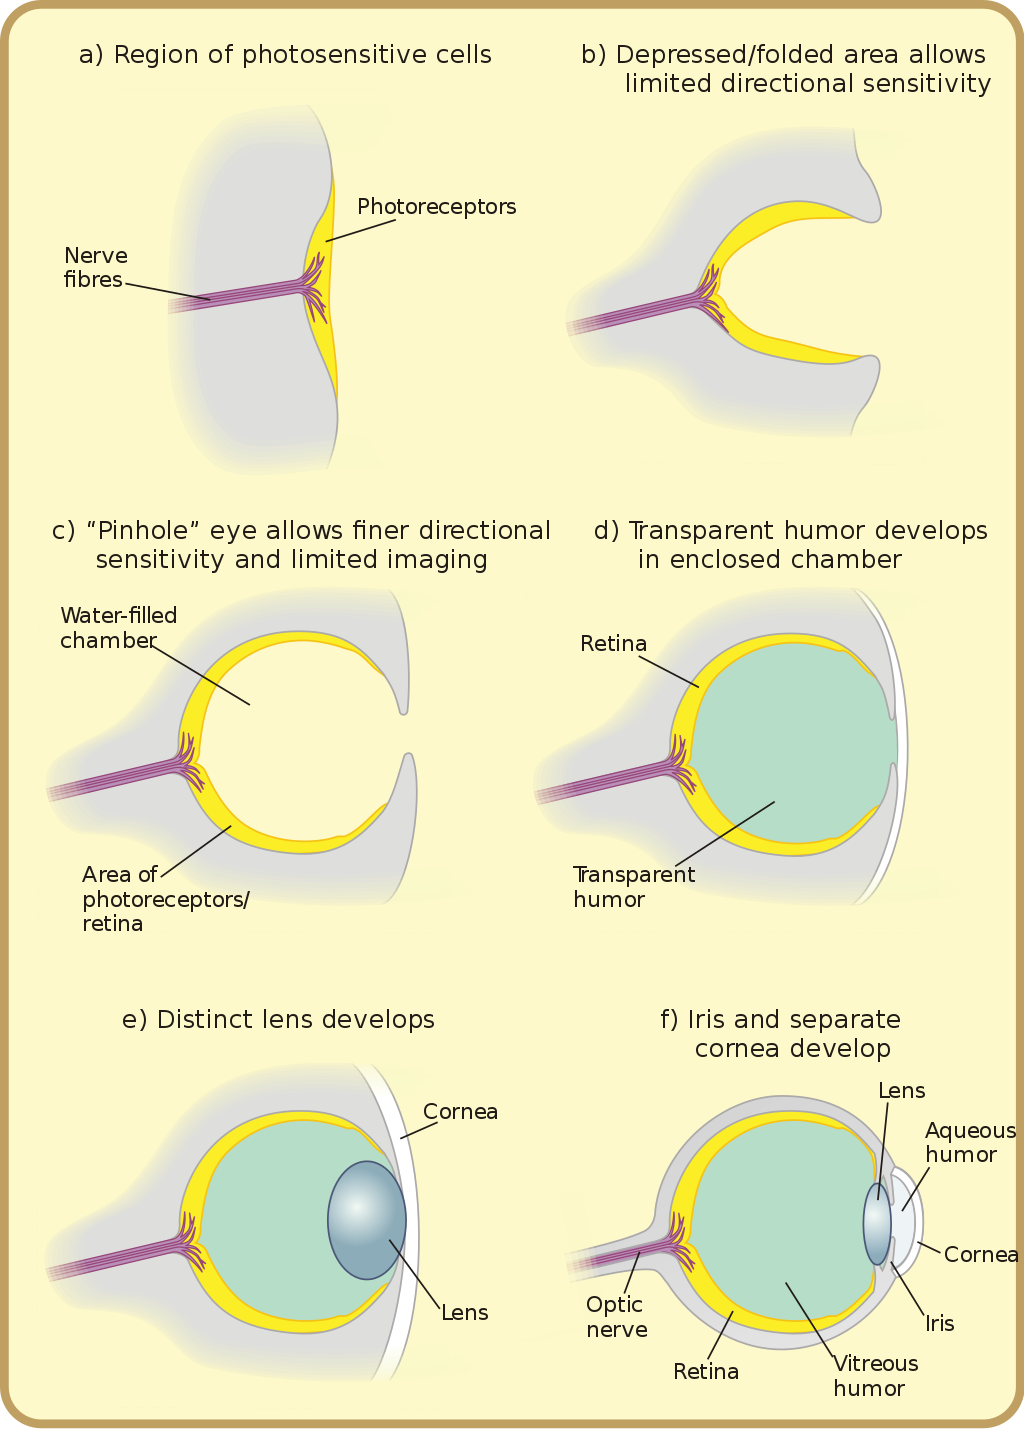
\includegraphics[width=0.45\linewidth]{./figs/evolutionEye} 

}

\caption{The evolution of an eye (Source: Wikipedia)}\label{fig:evolutionEye}
\end{figure}

Indeed,

\begin{itemize}
\item
  The eye is not developed by evolution with the purpose to see.
\item
  The eye only has the function to see.
\item
  It is the result of a gradual process where each adaptation gave a reproductive advantage in a particular environment.
\item
  In another environment it can be no longer functional and than it might disappear or might become dysfunctional, e.g.~moles eyes.
\end{itemize}

Hence, the origin of a species is the result of evolution, but, not the purpose of evolution. Evolution is thus adaptation with as sole goal maintenance and reproduction.

From the distribution of the complexity of species in Figure \ref{fig:distributionComplexity}, it is clear that the most abundant species in number always has been bacteria.
Indeed, evolution has no direction.
The distribution of complexity at present, however, has a tail to the right.
This mainly stems from the fact that there is lower bound of complexity of living organisms. Hence, evolution could not generate organisms with a complexity below this lower bound and it therefore only seems as if it slightly favors increasing complexity.



\begin{figure}

{\centering 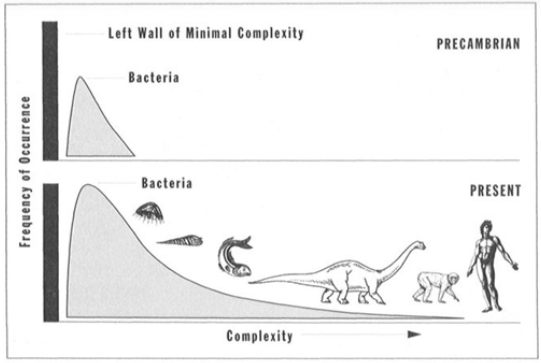
\includegraphics[width=0.45\linewidth]{./figs/selectionNoDirectionDef} 

}

\caption{Distribution of complexity of species \citep{gould1997}}\label{fig:distributionComplexity}
\end{figure}

\citet{Bar-On2018} published the distribution of carbon mass fixated in different types of species in Figure \ref{fig:carbonFixated}, which also shows that there is no preference towards more complex organisms.



\begin{figure}

{\centering 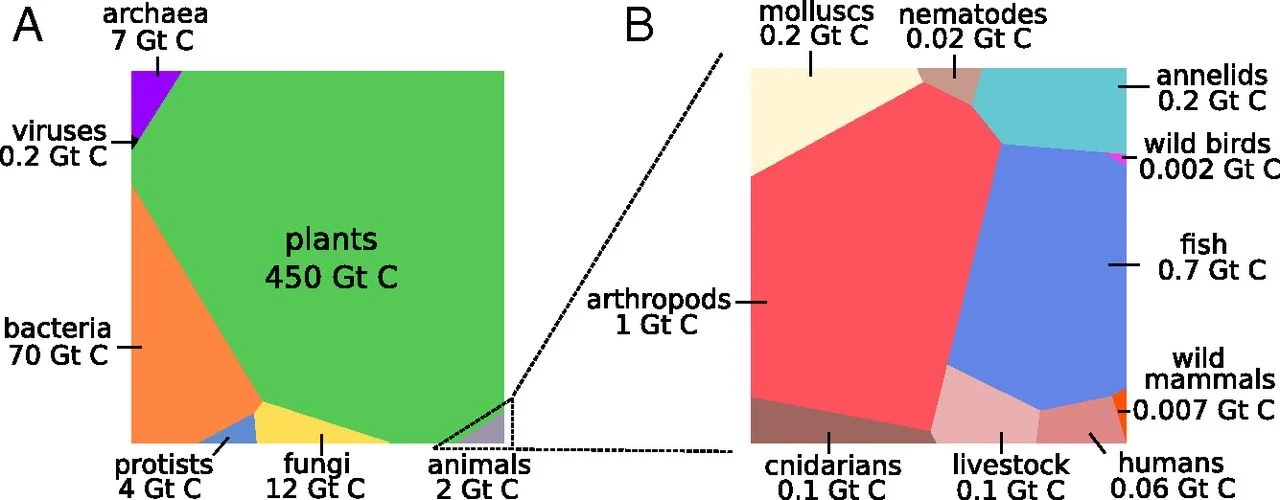
\includegraphics[width=1\linewidth]{./figs/pnas.1711842115fig01} 

}

\caption{Mass in giga tons of carbon for different groups of species. \citep{Bar-On2018}}\label{fig:carbonFixated}
\end{figure}

Note, that

\begin{itemize}
\item
  Plants are the most successful group in terms of the mass of carbon that they fixate.
\item
  Bacteria clearly dominate the more complex animal kingdom.
\item
  Animals represent a relative small fraction. Among animals, cattle and humans are over represented.
\end{itemize}

Other compelling evidence that there is no direction to evolution stems from the number of bacterial cells in our body. \citet{Sender2016} showed that the ratio of the number of bacterial cells to the number of human cells is close to 1. A human with a weight of 70kg has \(\pm\) 38 trillion bacterial cells and 30 trillion humane cells. Note, that trillion is a thousand billion or 10\(^{12}\)!

So, all these examples make clear that evolution has no direction. For every organism with a higher complexity there also emerge many organisms with lower complexity!

\hypertarget{evolution-of-evolution}{%
\section{Evolution of Evolution}\label{evolution-of-evolution}}

First there was

\begin{enumerate}
\def\labelenumi{\arabic{enumi}.}
\item
  Chemical evolution: the selection of building blocks and complex chemistry.
\item
  Then, biological evolution of cells/organisms based on the selection of genetic information and function.
\item
  And finally, our species introduced cultural evolution that can bypass natural evolution using

  \begin{itemize}
  \tightlist
  \item
    artificial selection: breeding of plants, pets, cattle, genetic manipulation, etc.
  \item
    Technology: that enables us for a fast adaptation to new environments
  \end{itemize}
\end{enumerate}

As a final remark, Rolando Toro also shared the view that the genetic information of a species can be seen as a record of the environments and development that it underwent up to this point.

Now that we introduce how all species could evolve from their last universal common ancestor we are ready to make the transition to how we humans evolves in our life span. This is also referred to as ontology, which is a another crucial biological aspect in the Model of Biodanza, which is our focus in the next chapter.

\hypertarget{ontogenesis}{%
\chapter{Ontogenesis}\label{ontogenesis}}

In the middle of the model, we see the biological aspect ``ontogenesis'' indicated with the red box in Figure \ref{fig:modelOnto}, which is our focus in this chapter.

\begin{figure}

{\centering 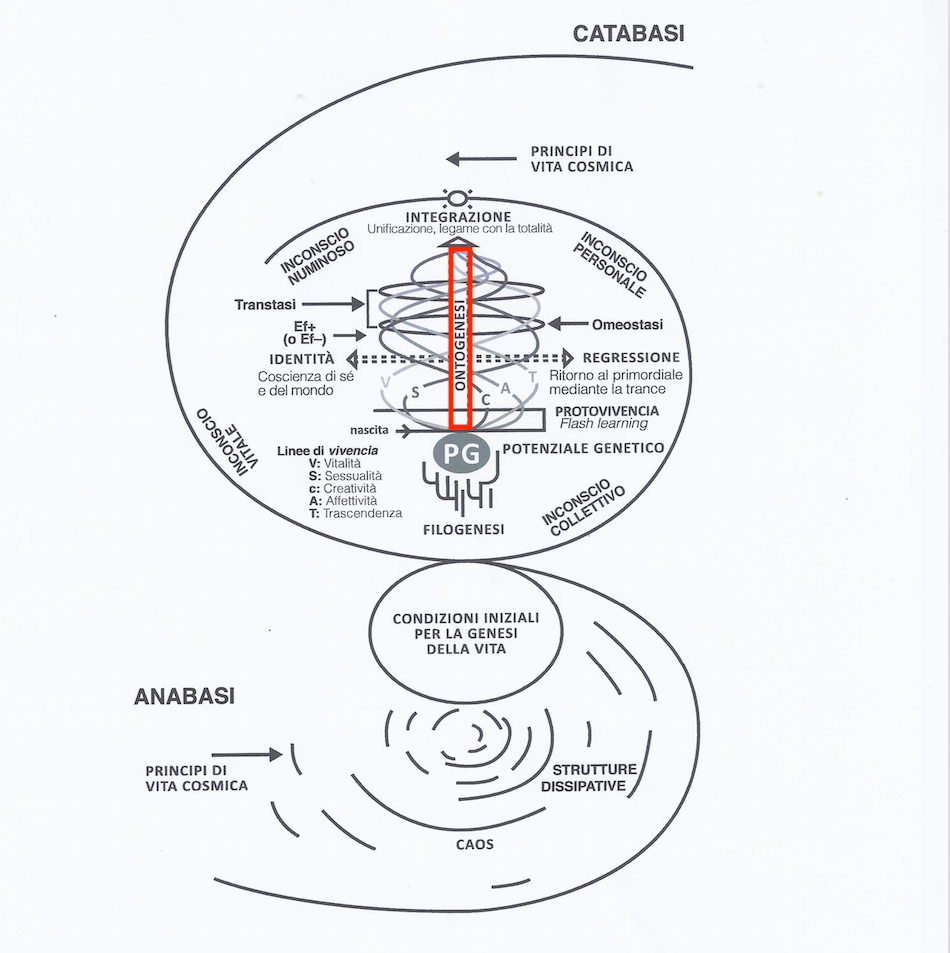
\includegraphics[width=0.5\linewidth]{./figs/biologischeAspectenBiodanzaDeelIII} 

}

\caption{Model of Biodanza and Ontogenesis}\label{fig:modelOnto}
\end{figure}

The ontogenesis is the development of an organism from a fertilized egg cell up to the adult stage until we eventually die.
We all start from the genetic potential we inherit from our parents through their egg and sperm cell.

The fertilized egg cell then starts to divide and at a certain point the cells start to differentiate into different tissues.
Each of our cells, apart from our germ cells, has the same genetic material!

A first question that arises is how cells of different tissues of the same organism that share the same genetic code can be morphologically so distinct? This is due to epigenetics!

\hypertarget{epigenetics}{%
\section{Epigenetics}\label{epigenetics}}

Epigenetics is the study of how development, behavior and environment can cause changes that affect the way we use our genes. Unlike genetic changes, epigenetic changes are reversible and do not change your DNA sequence, but they can change how our body can (or cannot) read a DNA sequence, see Figure \ref{fig:epigenetics}.

\begin{figure}

{\centering 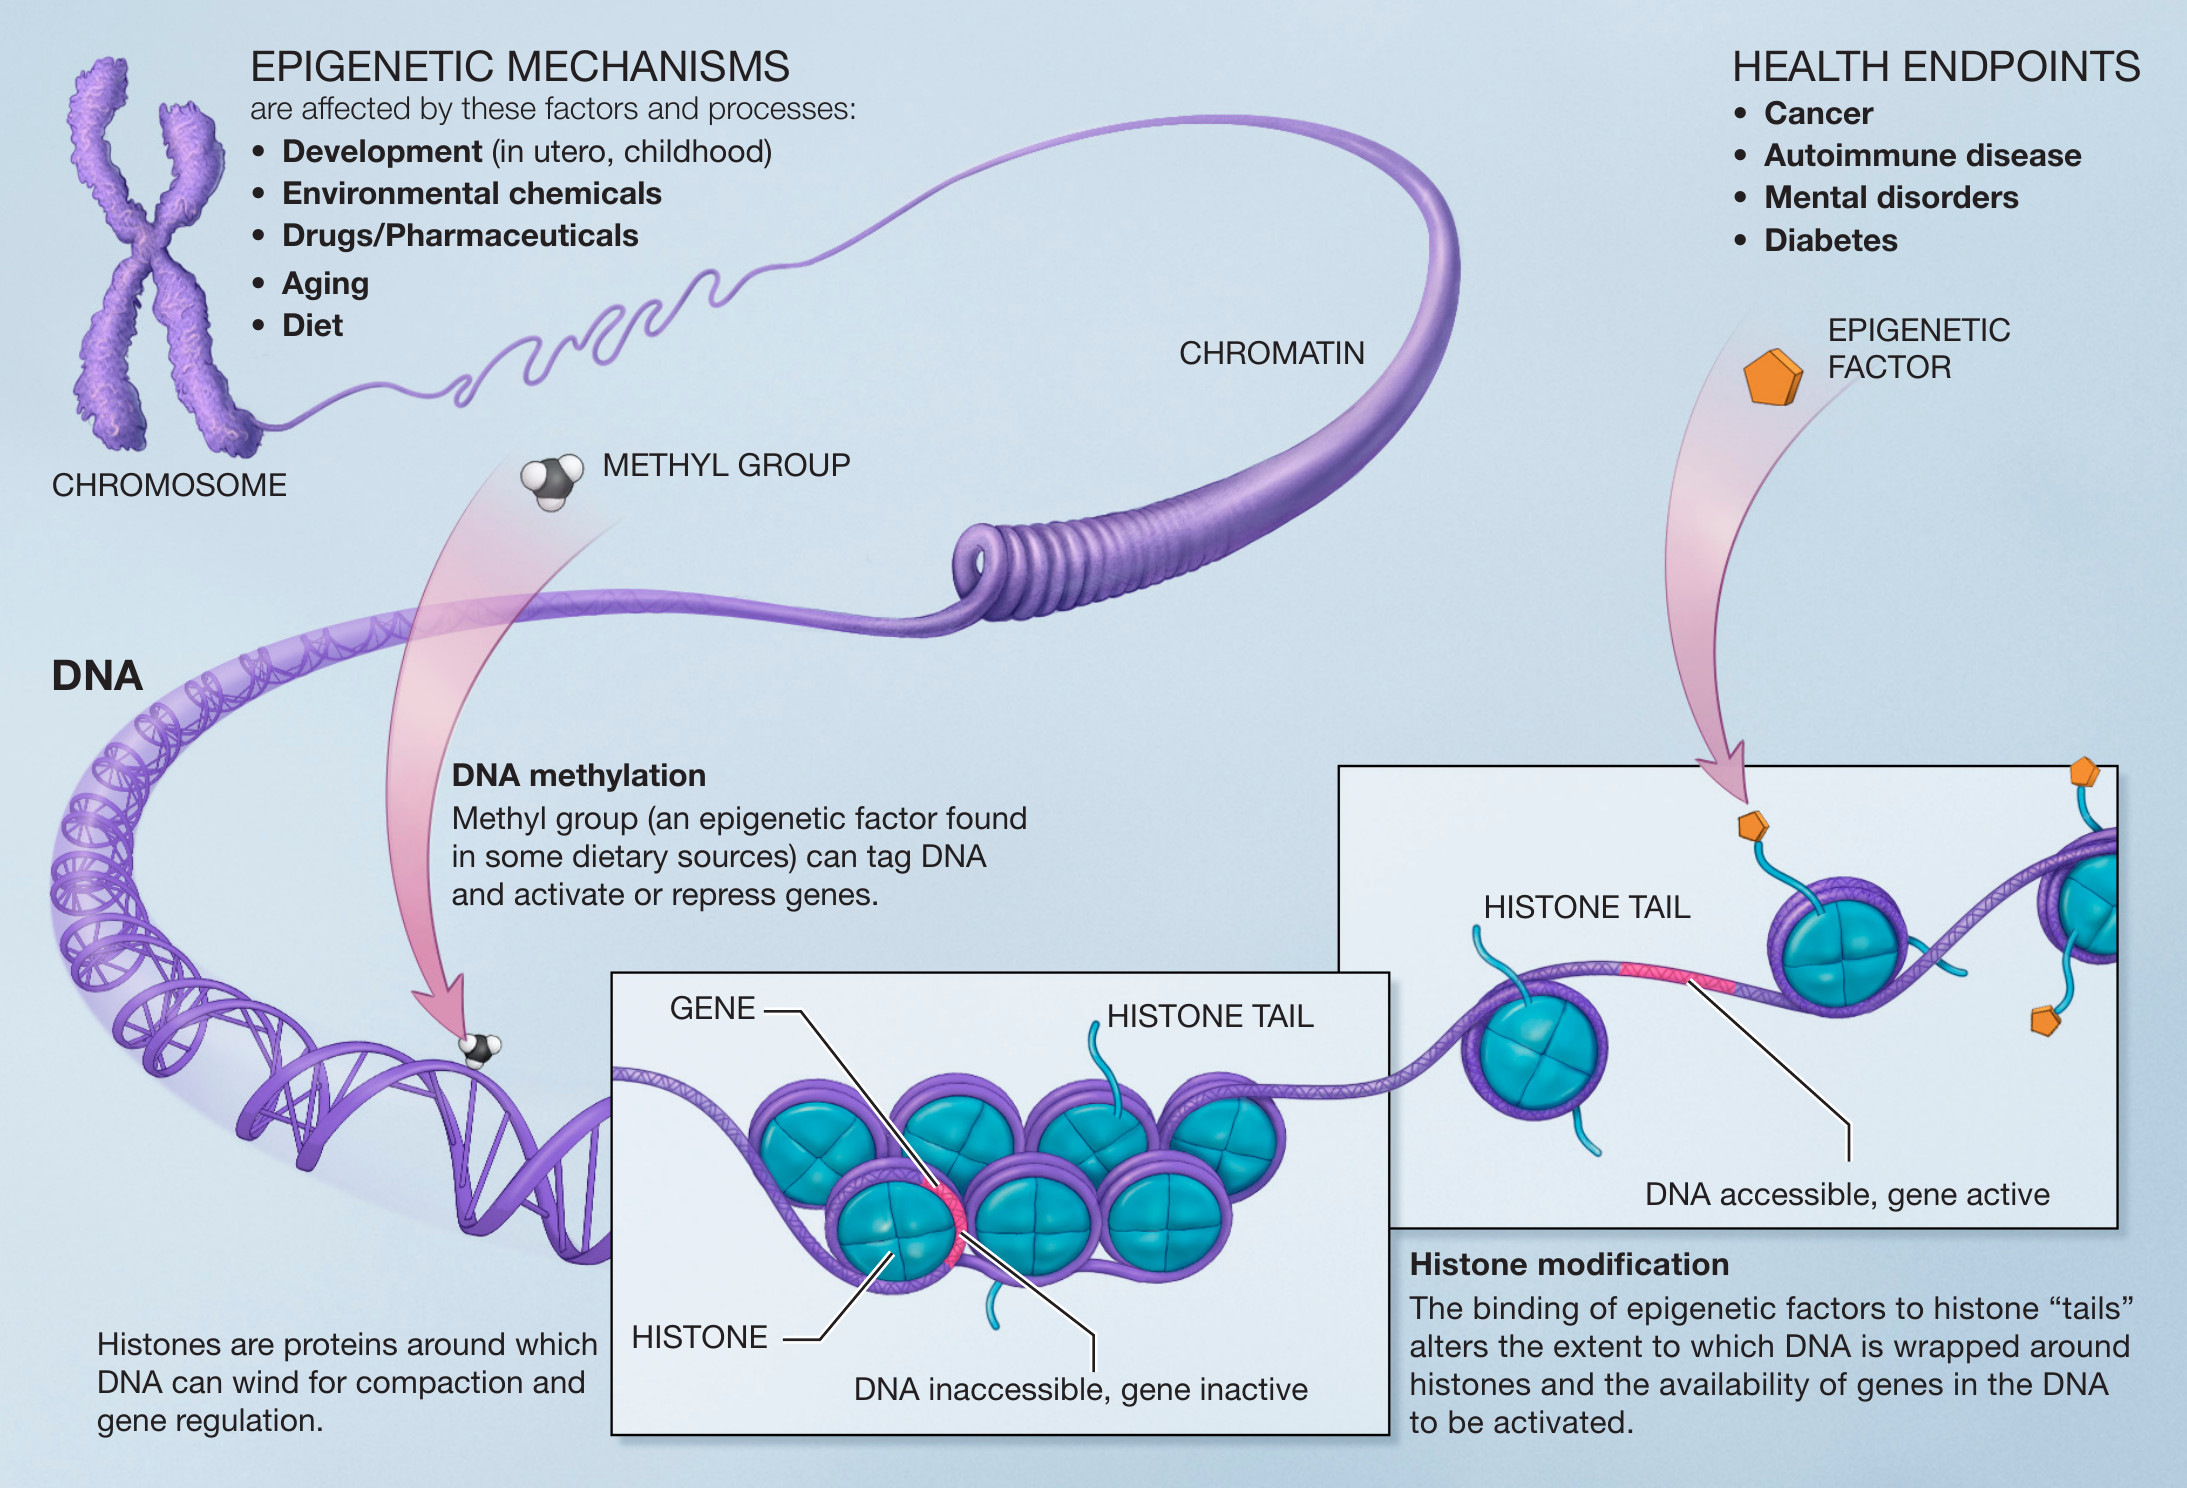
\includegraphics[width=1\linewidth]{./figs/Epigenetic_mechanisms} 

}

\caption{Principes of epigenetics. Small molecules, epigenetic markers, interact with the DNA and histones. They can cause a gene to be accessible or inaccessible for RNA transcription (Source: NIH, Wikipedia)}\label{fig:epigenetics}
\end{figure}

Epigenetic markers, however, are copied during cell division to the two new cells that are formed. This causes a liver cell to remain a liver cell and a brain cell to remain a brain cell upon cell division.

Epigenetic markers are small molecules that either interact directly with the DNA or through histones, proteins that act as spools that wind the long DNA molecule in a more compact/condense form.
They can make genes accessible or inaccessible for RNA transcription and thus eventually for the production of proteins. Two common types are

\begin{itemize}
\tightlist
\item
  DNA methylation: binding a methyl group directly to DNA (a methyl group (-CH\(_3\)) consists of one carbon and three hydrogen atoms).
\item
  Histone acetylation: binding an acetyl group to histone proteins (an acetyl group (-CO-CH\(_3\)) consists of two carbon, one oxygen and three hydrogen atoms).
\end{itemize}

Both types can impact the activity of genes.
On the one hand DNA methylation actively represses the expression of a specific gene, while DNA demethylation enhances gene expression.
On the other hand histone acetylation makes the structure of a region of DNA more open and thus more accessible for transcription of the genes in that region, while de-acetylation has the opposite effect.

\hypertarget{epigenetics-during-embryonal-development}{%
\section{Epigenetics during Embryonal Development}\label{epigenetics-during-embryonal-development}}

Epigenetics plays an important role in embryonic development (see Figure \ref{fig:epiEmbryo}).



\begin{figure}

{\centering 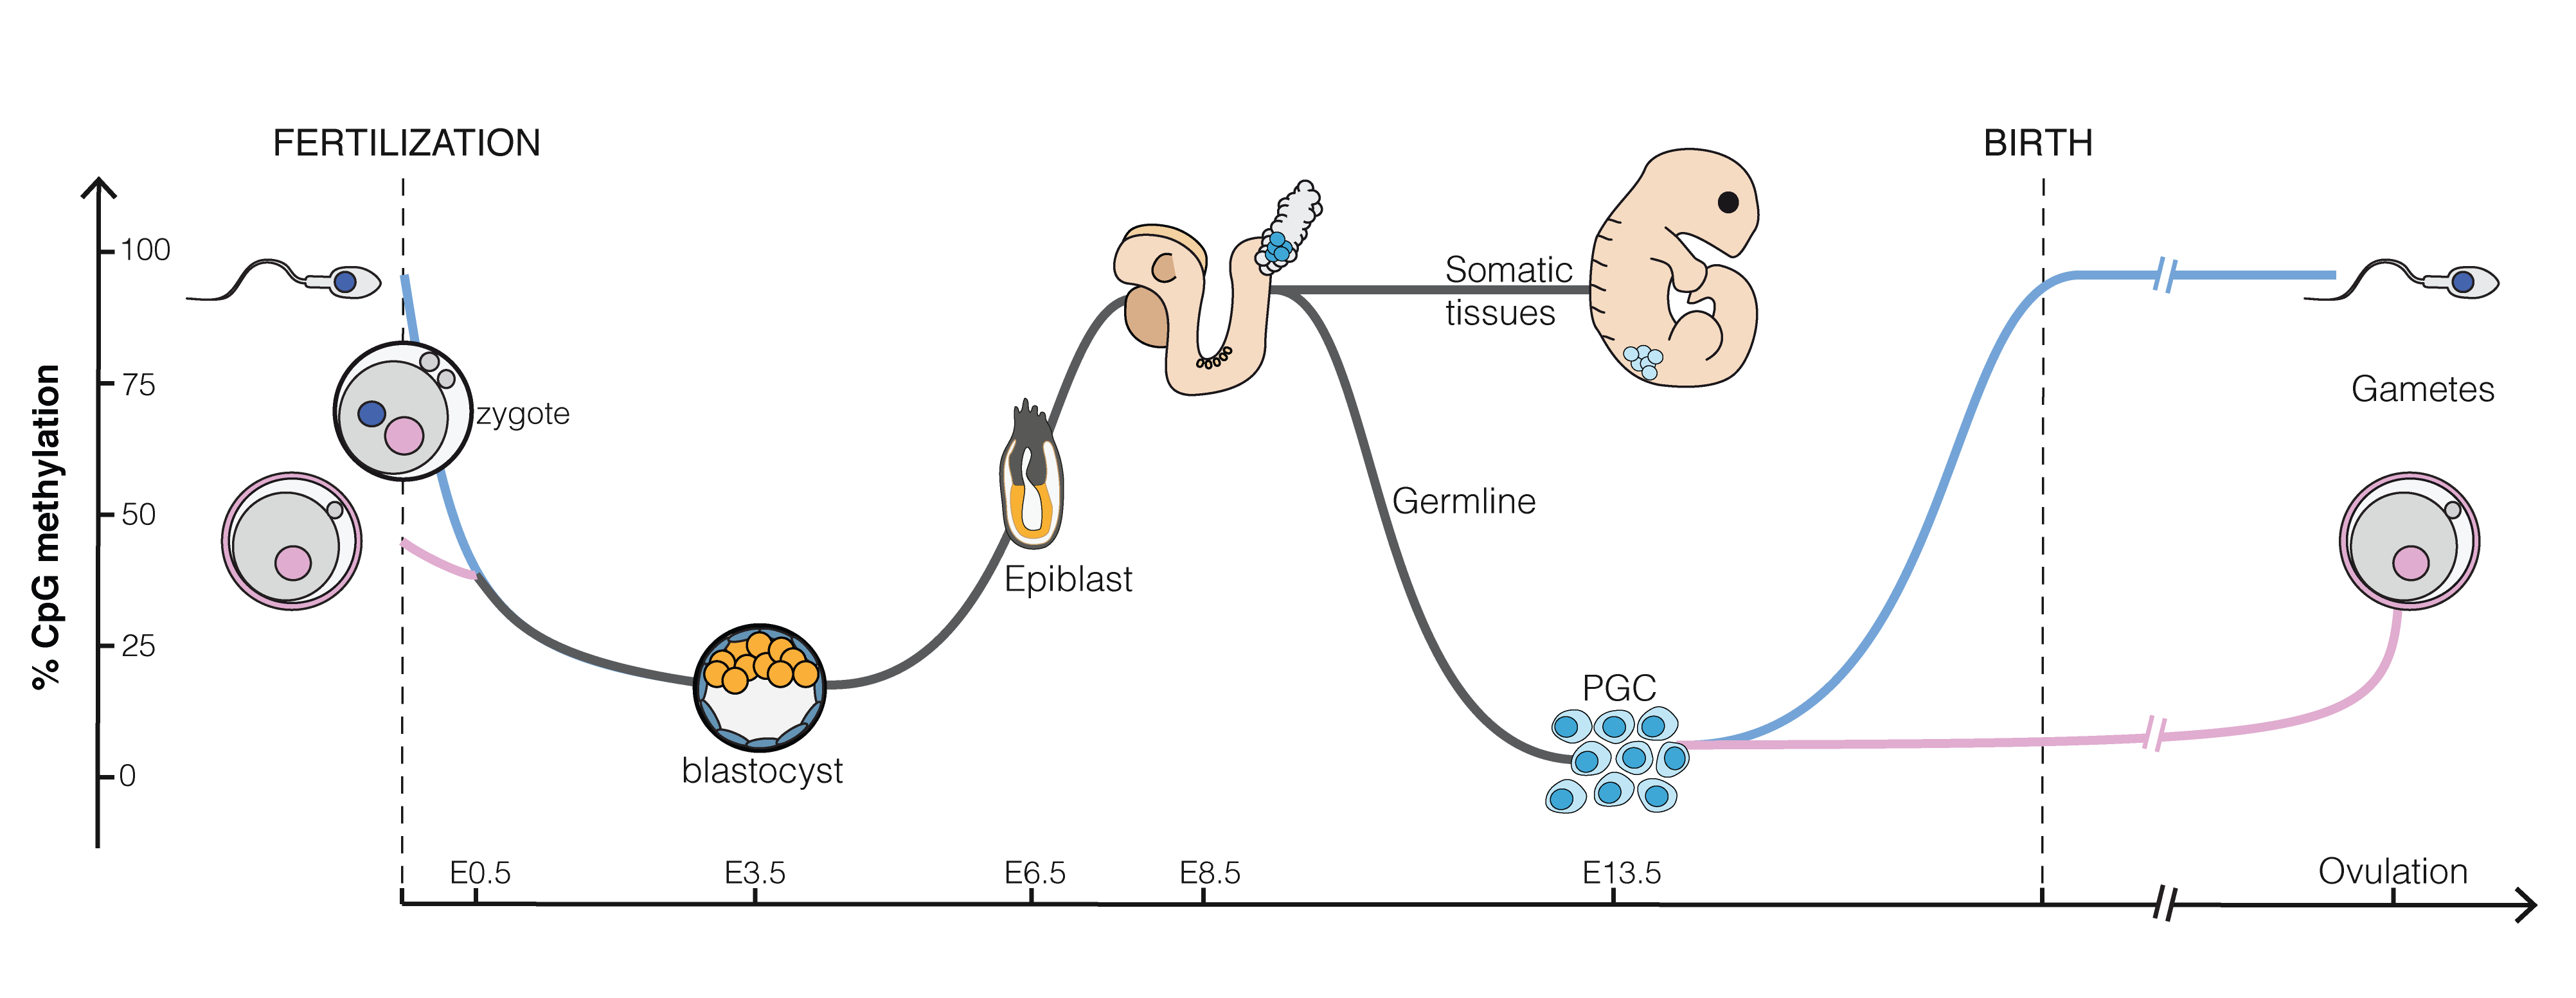
\includegraphics[width=1\linewidth]{./figs/DNA_methylation_reprogramming} 

}

\caption{Epigenetics in embryo genesis at CpG islands, regions that can bind with many methyl groups. All CpG islands of a sperm cell are almost fully methylated. That of an egg cell are methylated around 50\%. Upon fertilization the methylation drops and almost all genes become accessible for the undifferentiated blastula. As cells differentiate and get specific functions in tissues methylation increases again (Source: Mariuswalter, Wikipedia)}\label{fig:epiEmbryo}
\end{figure}

CpG islands are regions in our DNA that can be heavily methylated. All CpG islands of a sperm cell are almost fully methylated and few genes are accessible. Indeed, a sperm cell has one main function and that is to swim forward and fertilize the egg cell. The CpG islands of an egg cell are methylated around 50\%. Upon fertilization the methylation drops and almost all genes become accessible for the undifferentiated blastula (clump of undifferentiated cells). As differentiation of the cells starts and as they evolve into tissues and thus get specific functions, methylation increases again. This because only a subset of the genes has to be accessible for a differentiated cell to carry out its function. The methylation also has the advantage that it is passed upon cell division, which leads to invariance of differentiated cells: indeed, a liver cell remains a liver cell upon division and a brain cell a brain cell, etc.

\hypertarget{epigenetics-and-learning}{%
\section{Epigenetics and Learning}\label{epigenetics-and-learning}}

This section is largely based on the review article of Creighton et al.~entitled ``Epigenetic Mechanisms of Learning and Memory: Implications for Ageing'' \citep{Creighton2020}.

In the last decade, it has been shown that epigenetics is very important in development of the brain and for learning.

Animal research has shown that the disruption and inhibition of gene transcription to RNA and translation to proteins in the brain shortly after a learning event has a tremendous impact on long time memories (\(\geq 24\) hours), but not on short term memories. These manipulation had most impact in the first hours upon the learning event. Suggesting that the initial memory consolidation happens within a 6 hour time window.

Learning typically happens in waves. Genes activated shortly after learning return to baseline within 24 hours, a time point at which a second wave of gene expression is triggered.
In the second wave genes are included that encode for epigenetic regulators.
So, the first wave within 6 hours upon learning is known to upregulate transcription factors important to initiate the second wave of transcription, which is needed to establish long-lasting memories.

Understanding memory consolidation gets even more complex due to the reorganization of neural networks associated with recent memory storage and later memory phases (\(>7\) days).

\hypertarget{dna-methylation-and-memory}{%
\subsection{DNA Methylation and Memory}\label{dna-methylation-and-memory}}

In a large number of studies, DNA methylation has been shown to play an important role in multiple stages of memory formation.

On the one hand it is shown that DNA methylation is transient, i.e.~rapidly induced and reversed in the first hours upon learning. On the other hand, stably altered cortical DNA methylation has been shown up to 4 weeks upon learning and blocking the cortical DNA methylations has been shown to impair memory.
So methylation plays a role in different stages of the process of memory formation.

It also has been shown that methylation influences memory through different mechanisms, e.g.~

\begin{itemize}
\tightlist
\item
  Regulation of the activity of enhancers, i.e.~short DNA regions that enhance the transcription of proteins
\item
  Alternative splicing, i.e.~transcribed RNA from a gene region is spliced by which certain coding stretches can be removed, resulting in the production of different gene products from the same gene. So methylation can change the gene product that is transcribed from a particular gene.
\item
  Expression of micro RNAs, short non coding RNAs, that are biologically active.
\end{itemize}

A large body of literature support the role of methylation in learning and it is shown that methylation associated to learning occurs in the hippocampus, prefrontal cortex and the amygdala of the brain.

\hypertarget{histone-modifications-and-memory}{%
\subsection{Histone Modifications and Memory}\label{histone-modifications-and-memory}}

Another type of epigenetic regulation is through the modification of histones, i.e.~the proteins that act as spools around which the long DNA molecule is winded and which can affect the accessibility of a DNA region upon modification.

Histone modifications with epigenetic markers have been shown to be mainly important in the initial phase of memory consolidation. They are rapidly modified after which they return to baseline. These modifications cause ``winding or unwinding the DNA that is coiled around the histons'' making particular genes accessible or inaccessible for expression.

Histone epigenetic markers seem to regulate the transcriptional sensitivity towards external stimuli. Histone acetylation for instance has been shown to increase learning induced gene expression and seem to be particularly important for regulating memory strength.

\hypertarget{histon-variants-and-memory}{%
\subsection{Histon Variants and Memory}\label{histon-variants-and-memory}}

Histone variants, i.e.~histones with different amino acid chains, have recently been shown to be important novel regulators of neural plasticity, i.e.~the ability of the nervous system to change its activity in response to internal and external stimuli by reorganizing its structure, functions, or connections. Similar to histone modifications their dynamic nature is key for memory formation.

Recent progress has shown the tremendous importance of epigenetics for brain development and learning, however, the field of neuro-epigenetics is still in its infancy and many open questions remain.

\hypertarget{epigenetics-and-aging}{%
\section{Epigenetics and Aging}\label{epigenetics-and-aging}}

Epigenetics are also largely driven by ecofactors. This can be nicely illustrated with identical twins who have almost the same genome (only very small differences have been build up in the womb). It gets more easy to tell them apart over time due to epigenetic changes that are triggered by the different environments to which they were exposed. A good example is the difference in skin ageing between twins that had a different exposure to UV radiation (e.g.~Figure \ref{fig:epiUV}).



\begin{figure}

{\centering 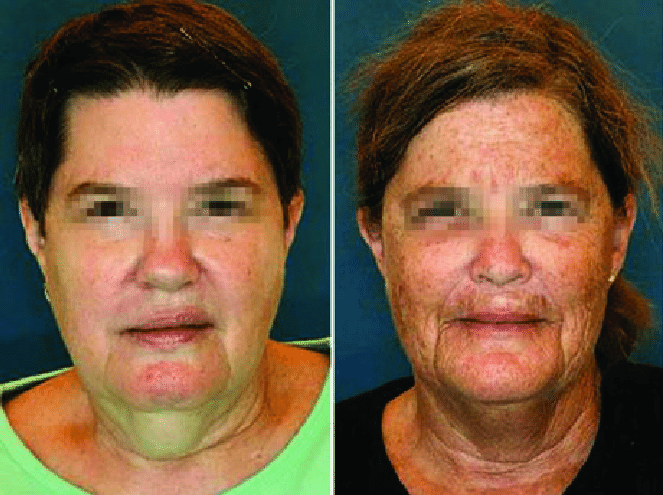
\includegraphics[width=0.5\linewidth]{./figs/dentical-twins-with-phenotypic-discordance-due-to-environmental-exposure-Although-MZ} 

}

\caption{Difference in skin ageing between twins is largely induced by epigenetic changes originating from a difference in exposure to UV radiation \citep{Schwab2017}}\label{fig:epiUV}
\end{figure}

Aging and longevity are influenced by genetic, epigenetic, and environmental factors during development, growth, maturity, and older stages.
It has been shown that the genetic component (heritability) plays only a moderate role in aging and longevity, so epigenetics seems to be a major contributor \citep{Adwan2018}. Indeed, many epigenetics markers and in particularly DNA methylation sites have been shown to be remarkable predictors of chronological age.
Aging has been shown to be associated
with profound changes in the epigenetic landscape, that give rise to alterations of gene expression and genome architecture.

An important modes of action in ageing has been shown to be through the association of epigenetics and telomere length.

Telomeres are regions of repetitive nucleotide sequences associated with specialized proteins at the ends of our chromosomes, see Figure \ref{fig:telomeres}. Each cell division the telomeres get shorter and the telomere shortening has been associated with ageing of tissues and organs.

\begin{figure}

{\centering 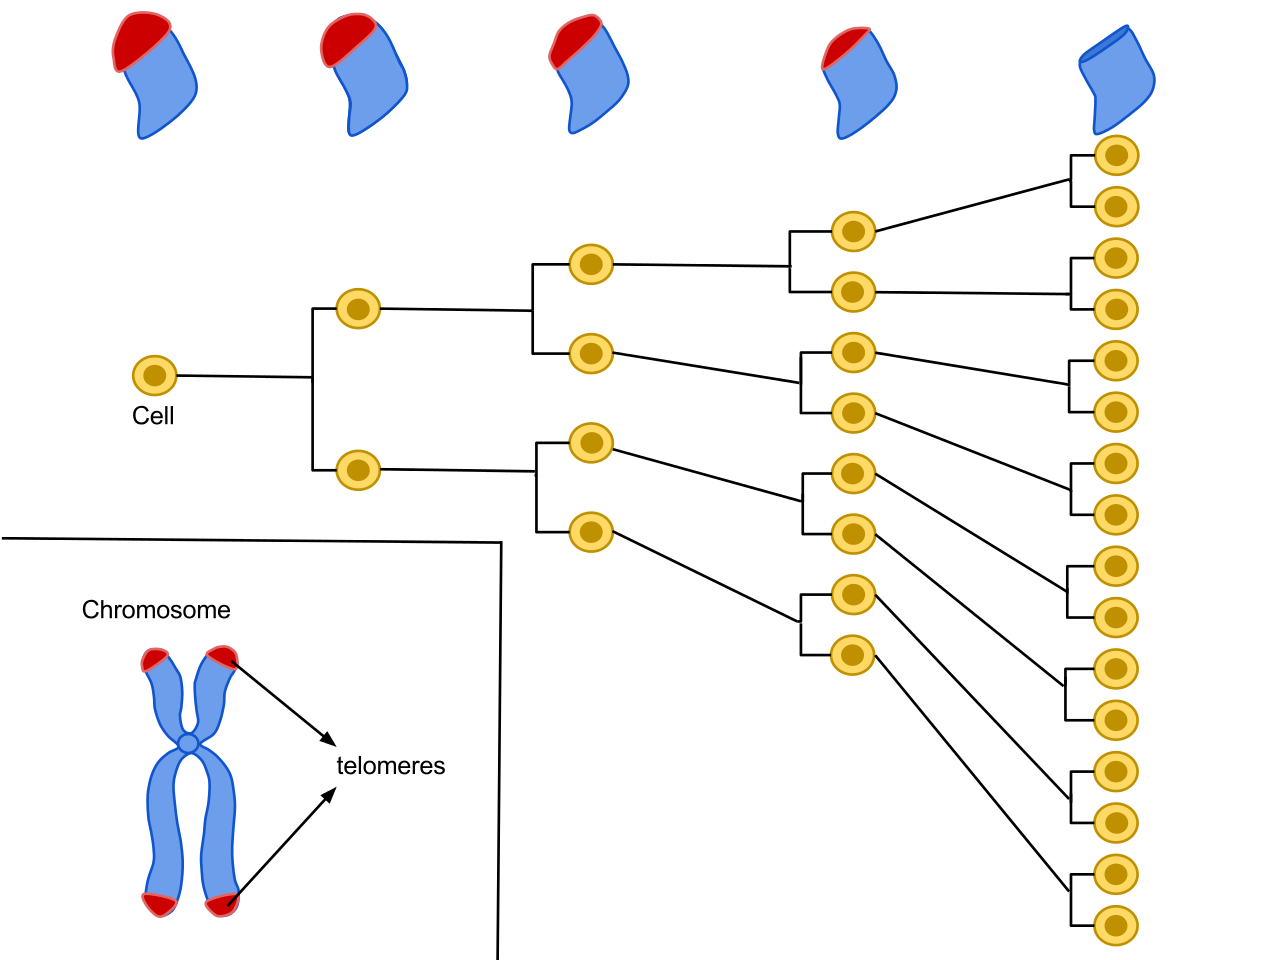
\includegraphics[width=0.8\linewidth]{./figs/telomeres} 

}

\caption{Telomeres are repetitive nucleotide sequences at the end of a chromosome. Each time a cell divides the telomeres on the end of the chromosome get smaller. The average cell will divide between 50 and 70 times before cell death (Source: Wikipedia)}\label{fig:telomeres}
\end{figure}

\citet{BlackburnEpel2017} use the plastic ends of shoelaces as an analogy for telomeres. If these ends shorten, the shoelace is prone to start fraying. Indeed, if the telomeres are getting two short, the integrity of the chromosome is at risk in the next cell division. Therefore a cell with too short telomeres goes into senescence: it stops with cell division, which will eventually lead to cell death.

However, through an enzyme complex called telomerase, the telomeres can be extended. So in the shoes analogy telomerase is the glue with which we could restore the plastic caps of a shoelace.

There is growing evidence that telomeres play a role in age-related processes. Indeed, mutations in telomerase and telomere genes causing increased telomere shortening, occur in patients with age-related disease, such as degenerative organ failure and a cancer-prone state among others. Moreover,
with genetically modified animal models causal links between telomere loss, cellular senescence (increasing cell death rates) and aging have been established \citep{Adwan2018}.

Epigenetics has also been shown to play an important role in telomere maintenance \citep{Adwan2018}.
Multiple studies showed that telomeric and subtelomeric regions contain histone modifications and subtelomeric DNA can undergo methylation.
Here, the epigenetic modification does not induce changes in the expression of target genes but affects telomere length or telomere structure.
Moreover, genes involved in the production of telomerase also have been shown to be under the regulation of methylation.

\hypertarget{epigenetics-and-stress}{%
\section{Epigenetics and Stress}\label{epigenetics-and-stress}}

Epigenetic also have been shown to be a key mechanism by which stressors interact with the genome.
This leads to stable changes in DNA structure, gene expression, and behavior (e.g. \citet{Park2019}).

Interestingly, stress and depression are mainly
associated with epigenetic alterations in genes involved in mediating resilience, vulnerability to stress, and stress-response related genes (e.g. \citet{Park2019}).

In their book ``the telomere effect'' \citet{BlackburnEpel2017} give an overview of their studies on the impact of stress on telomere length and telomerase activity.
They introduce many compelling examples and study results that underpin that ageing effects are strongly impacted by stress during childhood as well as by long-lasting stress on later age. And this, through the mediation of telomerase activity and telomere length, which we argued to be largely under control of epigenetics in the previous section.

\citet{BlackburnEpel2017} also discuss studies where it was shown that mind-body techniques such as meditation, qigong and yoga, among others are stress reducing, have positive effects on our well-being, can prevent inflammation and can induce cell rejuvenation by (re-)activating the gene that is encoding for teleomerase, among others. These effects were observed in well designed experiments and are in line with the beneficial effects that Rolando Toro also envisioned to induce through his System of Biodanza.

In this chapter we have introduced the concept of ontogenesis and its place in the Model of Biodanza. In the next and concluding chapter, we will briefly touch upon how we can affect the ontogenesis with the System of Biodanza, which is the ultimate goal of facilitating Biodanza.

\hypertarget{concluding-remarks-ontogenesis-in-biodanza}{%
\chapter{Concluding Remarks: Ontogenesis in Biodanza}\label{concluding-remarks-ontogenesis-in-biodanza}}

Ontogenesis is the vertical axis and can be seen as the time axis in the model, see Figure \ref{fig:modelOnto2}.

\begin{figure}

{\centering \includegraphics[width=0.5\linewidth]{./figs/biologischeAspectenBiodanzaDeelIII} 

}

\caption{Model of Biodanza and Ontogenesis}\label{fig:modelOnto2}
\end{figure}

Vivencia is the core instrument of the methodology of Biodanza, which has a strong impact on our body and brain. Indeed sensations that we experience are having a physiological impact through the genes that encode for a diverse scala of proteins, hormones and neurotransmitters.

Similar to what was shown extensively for other body-mind techniques in well controlled experiments (see e.g. \citet{BlackburnEpel2017}), we can expect many health benefits when practicing Biodanza. Also note, that the effects described by \citet{BlackburnEpel2017} for other body-mind techniques are in line with what Rolando Toro envisioned: going from reducing stress, preventing and reducing inflammation, to cell rejuvenation, etc.

Vivencia also has the quality that it immediately accesses our embodied mind through experience while bypassing our cognitive mind. So it enables us to learn by strong experiences that directly tap into our personal, collective and vital unconsciousness.

The experiences through vivencia can be imprinted through the epigenetic mechanisms of learning and memory. Indeed, as Biodanza practitioners we are familiar with the long lasting memories to deep vivencia. Moreover, practicing Biodanza over a longer period also induces change.
Change in how we feel, stand in life, interact socially and with our environment.
This change is undoubtedly a result of rewiring of our brain and thus of how we effectively use our genetic potential.

Hence, with the methodology of Biodanza we have a very powerful tool to influence our ontogenesis, i.e.~the pulsation between regression and identity in the five lines of Biodanza through the gestalt: music, movement and vivencia.
This pulsation between regression and identity is essential because an organism tends to filter stimuli that are continuously present.

So in a typical Biodanza session,

\begin{itemize}
\tightlist
\item
  we first enhance our identity through vital exercises,
\item
  subsequently we slow down our movement and lower our state of control in exercises on regression and transcendence, which deeply connect us with our personal, collective and vital unconsciousness and promote strong vivencia.
\item
  Finally, we stimulate our vivencia to be imprinted in our long term memory during the positive vibes in the reactivation and vital exercises at the end of the session.
\end{itemize}

With the repetition of exercises across multiple sessions we effectively strengthen this imprinting further and eventually can promote immense personal growth and this in the five lines of Biodanza.

\newpage

\hypertarget{postface}{%
\chapter*{Postface}\label{postface}}
\addcontentsline{toc}{chapter}{Postface}

This writing was my humble attempt to convey my passion for the system of Biodanza and vibrating it to you. I hope that I was able to

\begin{itemize}
\tightlist
\item
  lay out the strong foundation of the System of Biodanza in the life sciences,
\item
  link these biological aspects clearly to all relevant parts in the Model of Biodanza, and
\item
  provide a better insight in these biological aspects for Biodanza practitioners and facilitators who do not have a formal training in the life sciences.
\end{itemize}

I also hope that this monograph will trigger you to continue with your Biodanza practice with even more enthusiasm. Indeed, it is a unique path to promote your ontogenesis and well-being, and, has the promise to impact your personal development considerably. Moreover, it might also change the larger autopoietic social system in which you are embedded. And this, as Rolando Toro envisioned, by effectively switching it to another attractor through its positive feedback on your change, growth and interaction.

  \bibliography{bibliography.bib}

\end{document}
